\section{Estimation of Deterministic parameters: Method of Moments and Maximum likelihood estimators}

\subsection{Estimation of Deterministic Parameters}

\begin{itemize}
    \item \textbf{Question:} Does it exist an estimator that is the most efficient? i.e. an estimator that has the lowest MSE?
    \[
    \textbf{Minimum Mean Square Error (MMSE) Estimator}
    \]
    \item For example, assume we want to estimate the mean value \(\eta\) of a r.v. \(X\) given a vector of \textbf{X} of independent observations, i.e. \(\{X_i\}\) are \(N\) IID r.v.'s: Does it exist an estimator that is more efficient than the \textbf{Sample Mean}?
    \item Let us suppose that if it exists it has the following structure:
 \[
\hat{\eta} = \frac{\alpha}{N} \sum_{i=1}^N X_i = \alpha \overline{X}
\quad \Rightarrow \quad \text{if } \alpha = 1 \ \rightarrow \ 
\hat{\eta} = \overline{X} \equiv \text{Sample Mean}
\]

\[
\text{where} \quad
\overline{X} \triangleq \frac{1}{N}\sum_{i=1}^{N} X_i 
\quad \text{is the Sample Mean}
\]
    \item What is the value of \(\alpha\) that minimizes the MSE?
\[    \overline{X} \triangleq \frac{1}{N} \sum_{i=1}^{N} X_i 
\implies 
E\left\{\overline{X}\right\} = \eta, \quad
\mathrm{var}\left\{\overline{X}\right\} = \frac{\sigma^2}{N}
\]

\[
MSE(\alpha) = E\left\{ (\hat{\eta} - \eta)^2 \right\}
= E\left\{ (\alpha \overline{X} - \eta)^2 \right\}
= \alpha^2 E\left\{ \overline{X}^2 \right\} 
- 2\alpha\eta E\left\{ \overline{X} \right\} + \eta^2
\]

\[
= \alpha^2 \left( \eta^2 + \frac{\sigma^2}{N} \right)
- 2\alpha \eta^2 + \eta^2
\]

\[
\frac{d MSE(\alpha)}{d \alpha} = 2\alpha \left( \eta^2 + \frac{\sigma^2}{N} \right) - 2\eta^2
\]

\[
\min_{\alpha} MSE(\alpha) \iff \frac{d MSE(\alpha)}{d \alpha} = 0
\]    
$$
\min_{\alpha} MSE(\alpha) \iff \frac{d MSE(\alpha)}{d \alpha} = 0
$$

$$
\frac{d MSE(\alpha)}{d \alpha} = 2\alpha \left( \eta^2 + \frac{\sigma^2}{N} \right) - 2\eta^2 = 0 \implies \alpha = \frac{\eta^2}{\eta^2 + \frac{\sigma^2}{N}} = \frac{1}{1 + \frac{\sigma^2}{N\eta^2}}
$$



    Where \(\gamma\triangleq\frac{\eta^2}{\sigma^2}\) is a sort of SNR.\\
    Note that : \(0\leq \alpha_{MMSE}\leq1\) and \(\lim_{N\hspace{0.2em}or\hspace{0.2em}\gamma\rightarrow+\infty}\alpha_{MMSE}=1\)\\
    In practice if \(N\gg1\) or \(\gamma\gg1\)\(\longrightarrow\alpha_{MMSE}=1\)
$$
\hat{\eta}_{MMSE} = \alpha_{MMSE} \cdot \frac{1}{N} \sum_{i=1}^N X_i
\rightarrow b\left\{ \hat{\eta}_{MMSE} \right\} = E\left\{ \eta - \hat{\eta}_{MMSE} \right\} = \eta - \alpha_{MMSE} \eta
$$

$$
b\left\{ \hat{\eta}_{MMSE} \right\} = (1 - \alpha_{MMSE})\eta =
\left( 1 - \frac{1}{1 + \frac{1}{N\gamma}} \right) \eta = \frac{1}{1 + N\gamma}\eta \quad\quad \eta \neq 0
$$

$$
MMSE = MSE(\alpha_{MMSE}) = \frac{\sigma^2}{N} \cdot \frac{1}{1 + \frac{1}{N\gamma}}
= \alpha_{MMSE} \cdot \frac{\sigma^2}{N} \leq \frac{\sigma^2}{N}
$$


    \item The problem is that the structure of the optimal MMSE estimator depends on the unknown parameter \(\eta\) we want to estimate, so it cannot be implemented, i.e. it is not feasible.
    \item In other words, it does not exist an estimator that is optimal(minimum MSE) whatever is the value of the unknown parameter we want to estimate.
    \item The results we have just derived tell us that the \textbf{Sample Mean} is non optimal but asymptotically optimal(i.e. for \(N\rightarrow\infty\) or \(\gamma\rightarrow\infty\)), in fact for \(N\gg1\) or \(\gamma\gg1\) the unfeasible MMSE estimator and the Sample Mean coincide.
    \item Since \underline{an MMSE estimator for the estimation of deterministic parameters does not exist}, we should look for other methods (in addition to the \textbf{Sample Estimators} that we have already introduced, which are suitable for some specific estimation problems).
    \item These other methods should provide feasible estimators, that even if sub-optimal, have good performance, i.e. close as possible to the optimal one.
    \item One of the simplest and most widely adopted methods is the \underline{\textbf{Method of moments(MM)}}.
    \item We start assuming a specific statistical model, i.e. a specific pdf , for our discrete observed data. The observed data should depend on the parameter we want to estimate, so as a consequence also their pdf: \(\textbf{X}(\theta)\rightarrow f_{\textbf{X}}(\textbf{x};\theta)\)

\end{itemize}
\subsection{Method of Moments}
\begin{itemize}
    \item Once we assume a specific pdf model(Gaussian,Laplace, Exponential, Weibull, Chauchy, t-student, etc), the model is completely specified, except for a number of unknown deterministic paramter \(\theta\), that must be derived in such a way to match at the "best" the theoretical model to the observed data \(\rightarrow\)it is a \textit{data fitting} problem.
    \item \textbf{Assumption}: the \(N\) observed data \(\{X_i\}\) are independent realizations of a r.v. \(X\).
    \item Let us calculate the relationship between the unknown parameter \(\theta\) and one of the moments of the r.v. \(X\), e.g. the mean value:
$$
m_1 \triangleq E\left\{ X \right\} = \int_{-\infty}^{+\infty} x f_X(x; \theta) dx \implies m_1 = h_1(\theta)
$$

    \item If this relationship can be inverted, we can express the unknown parameter \(\theta\) as a function of the mean value of \(X\):
    \[
    \theta=h_1^{-1}(m_1)
    \]
    \item Since the mean value \(m_1\) is unknown a priori, we cannot derive the true value of \(\theta\) from this relationship. However, we can replace the unknown mean value with its estimate, e.g. obtained by using the \textbf{Sample Mean} estimator:
    $$
\theta = h_1^{-1}(m_1) \implies \hat{\theta}_{MM} = h_1^{-1}(\hat{m}_1)
\qquad \text{where} \qquad \hat{m}_1 \triangleq \frac{1}{N} \sum_{i=1}^{N} X_i
$$
    \item The estimator we find in this way is called \textbf{Method of Moments(MM)} estiamtor. To analyze the estimation performance, we have to derive the estimator \(\textbf{bias}\) and \(\textbf{MSE}\).
    \item As concerning the \textbf{efficiency} of the estimator, we cannot say anything. However, since the Sample Mean is a \textbf{consistent} estimator, also the MM estimate of \(\theta\) is \textbf{consistent}(under mild conditions on the function \(h_1\)):
    $$
\lim_{N \to \infty} \hat{\theta}_{MM} = \lim_{N \to \infty} h_1^{-1}(\hat{m}_1) = h_1^{-1}\left( \lim_{N \to \infty} \hat{m}_1 \right) = h_1^{-1}(m_1) = \theta
$$


    \item The \textbf{Method of Moments} is fairly simple and yields \textbf{consistent} estimators (under very weak assumption), though estimators are often \textbf{biased}.
    \item In fact, the unbiasdness of the Sample Mean does not imply that the MM estimator of \(\theta\) is also unbiased:
 $$
E\left\{ \hat{\theta}_{MM} \right\} = E\left\{ h_1^{-1}(\hat{m}_1) \right\} \neq h_1^{-1}\left( E\{\hat{m}_1\} \right) = h_1^{-1}(m_1) = \theta
$$



    \item This is because \(h_1(.)\) and its inverse are in general non linear transformations.
    \item The \textbf{Method of moments} can be easily extended to the case of multiple unknown parameters:
    \[
    \boldsymbol{\theta}=[\theta_1\hspace{0.5em} \theta_2\hspace{0.5em}\cdots\hspace{0.5em}\theta_P]^T
    \]
    \item To estimate \(P\) unknown parameters we need at least \(P\) equations. We can obtain these \(P\) equations by calculating \(P\) moments of the pdf of \(X\).
    \item It is a good practice to calculate the mean and the first \(P-1\) central moments:
$$
\begin{cases}
    m_1 = E\left\{ X_i \right\} = h_1(\theta) \\
    \mu_2 = E\left\{ (X_i - m_1)^2 \right\} = h_2(\theta) \\
    \vdots \\
    \mu_P = E\left\{ (X_i - m_1)^P \right\} = h_P(\theta)
\end{cases}
\implies \boldsymbol{\mu} = \mathbf{h}(\theta)
$$

    \item IMPORTANT : System of \(P\) equations (generally nonlinear) with \(P\) unknowns.

    \item Solving the system of equations with respect to vector \(\theta\), we get the inverse relationship between the moments and the unknown parameter vector:
    \[
    \boldsymbol{\theta}=\textbf{h}^{-1}(\boldsymbol{\mu})
    \]
    \item Since the moments are not a priori known, we should replace their values with their estimates, obtained by using \textbf{Sample Estimators}:
$$
\hat{m}_1 \triangleq \frac{1}{N} \sum_{i=1}^N X_i, \qquad
\hat{\mu}_k \triangleq \frac{1}{N} \sum_{i=1}^N \left( X_i - \hat{m}_1 \right)^k, \quad k = 2,3,\ldots,P
$$

$$
\hat{\boldsymbol{\mu}} = \left[ \hat{m}_1 \quad \hat{\mu}_2 \quad \hat{\mu}_3 \quad \cdots \quad \hat{\mu}_P \right]^T
$$

$$
\implies \hat{\theta}_{MM} = \mathbf{h}^{-1}(\hat{\boldsymbol{\mu}})
$$


    \item \textbf{IMPORTANT}: The estimators obtained by the Method of Moments are \textbf{consistent}(under the very weak assumption that the central moments of \(X\) exists and are finite up to the order \(2P\)).

    \item \textbf{Example}: Estimate the parameter \(\eta\) of an Exponential pdf, given \(N\) independent realizations of the r.v. \(X\), assumed to be exponentially distributed.
$$
\mathbf{X}_{N \times 1} = \left[ X_1 \quad X_2 \quad \cdots \quad X_N \right]^T, \quad \left\{ X_i \right\}_{i=1}^N \quad \text{IID}
$$

$$
f_{X_i}(x_i) = \eta e^{-\eta x_i} u(x_i)
\rightarrow
m_1 \triangleq E\left\{ X_i \right\} = \frac{1}{\eta}, \qquad
\mu_2 \triangleq \mathrm{var}\left\{ X_i \right\} = \frac{1}{\eta^2}
$$

    \noindent The distribution is monoparametric (it depends on one parameter only). Hence, to estimate \(\eta\) we need only one moment. We can use for example the mean value or the variance:
$$
m_1 = E\left\{ X_i \right\} = \frac{1}{\eta} \implies \eta = \frac{1}{m_1} \implies \hat{\eta} = \frac{1}{\hat{m}_1}
$$

$$
\mu_2 = \mathrm{var}\left\{ X_i \right\} = \frac{1}{\eta^2} \implies \eta = \frac{1}{\sqrt{\mu_2}} \implies \tilde{\eta} = \frac{1}{\sqrt{\hat{\mu}_2}}
$$
    We obtain two solutions, which one of the should we use?
    $$
    \hat{\eta} = \frac{1}{\hat{m}_1} = \frac{1}{\frac{1}{N}\sum_{i=1}^N X_i}\qquad
    \tilde{\eta} = \frac{1}{\sqrt{\hat{\mu}_2}} = \frac{1}{\sqrt{ \frac{1}{N} \sum_{i=1}^N \left(X_i - \hat{m}_1\right)^2 }}
    $$
    \noindent The first estimator is simpler to implement(lower \textbf{computational complexity})\\
    \noindent We have to compare them in terms of \textbf{estimation accuracy}.\\
    \noindent It is difficult to obtain the pdf's of the two estimators in closed-form. We derived the \textbf{normalized histogram} of the two estimators by generating a large number \(M\) of realization of the estimates(the normalized histogram represents a non-parametric method to estimate the pdf of a r.v.).\\
    \noindent The pdf's have been obtained by generating \(M=10^6\) Monte Carlo runs.\\
    \noindent For \(N=10\), the second one is better, but for higher \(N\) the first estimator is always better(it's the one based on the Sample Mean, i.e. the moment of lowest order):
    \begin{figure}[H]
        \centering
        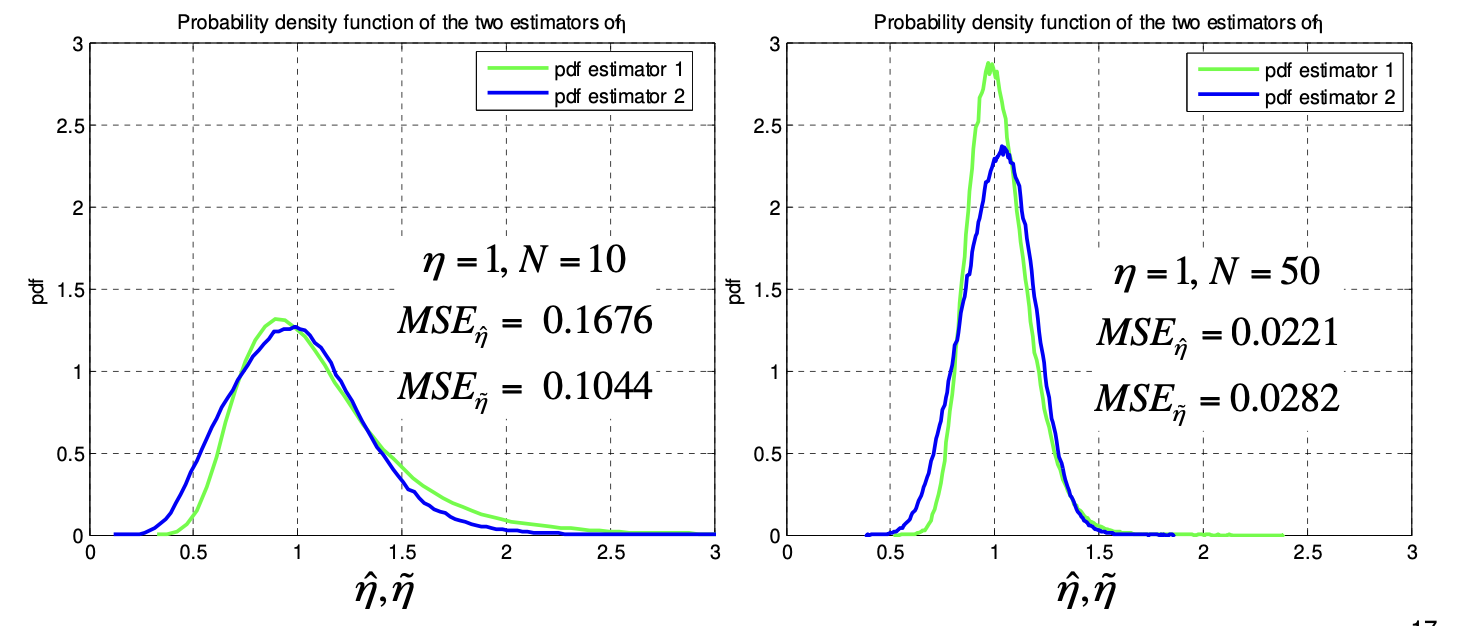
\includegraphics[width=0.75\linewidth]{Image/pdf 4/1.EXAMPLE_1.png}
        \label{fig:placeholder}
    \end{figure}
    \item \textbf{EXAMPLE 2}: Estimate two parameters \(a\) and \(b\) of a uniform pdf, given \(N\) independent realizations of the r.v. \(X\), assumed to be uniformly distributed between \(a\) and \(b\).
    $$
    \mathbf{X}_{N \times 1} = \left[ X_1 \quad X_2 \quad \cdots \quad X_N \right]^T, \quad \left\{ X_i \right\}_{i=1}^N \ \text{IID}, \quad f_{X_i}(x_i) = \frac{1}{b-a} \, \mathrm{rect} \left( \frac{x_i - \frac{a+b}{2}}{b-a} \right)
    $$

    $$
    \rightarrow \quad m_1 = E\left\{ X_i \right\} = \frac{a+b}{2}, \qquad \mu_2 = \mathrm{var}\left\{ X_i \right\} = \frac{(b-a)^2}{12}
    $$
    \noindent The distribution is biparametric, so ween at least two equations , i.e. we need to estimate at least two moments.\\
    \noindent We can obtain two equations by calculating the relationship between the mean value and the variance and the two parameters \(a\) and \(b\).\\
    \noindent Once we have two equations, we have to solve them with respect to parameters \(a\) and \(b\):

    $$
    \begin{cases}
    m_1 = E\left\{ X_i \right\} = \frac{a+b}{2} \\
    \mu_2 = \mathrm{var}\left\{ X_i \right\} = \frac{(b-a)^2}{12}
    \end{cases}
    \implies
    \begin{cases}
    b+a=2m_1 \\
    b-a=2\sqrt{3\mu_2}
    \end{cases}
    \implies
    \begin{cases}
    a = m_1 - \sqrt{3\mu_2} \\
    b = m_1 + \sqrt{3\mu_2}
    \end{cases}
    $$
    \noindent A this point, to obtain the MM estimate of parameters \(a\) and \(b\), we just have to replace in the above equations the true values with their \textbf{Sample estimates}:
    $$
\begin{cases}
    \hat{a}_{MM} = \hat{m}_1 - \sqrt{3\hat{\mu}_2}
    = \frac{1}{N} \sum_{i=1}^N X_i
    - \sqrt{ 3 \cdot \frac{1}{N} \sum_{i=1}^N \left( X_i - \hat{m}_1 \right)^2 }
    \\[1ex]
    \hat{b}_{MM} = \hat{m}_1 + \sqrt{3\hat{\mu}_2}
    = \frac{1}{N} \sum_{i=1}^N X_i
    + \sqrt{ 3 \cdot \frac{1}{N} \sum_{i=1}^N \left( X_i - \hat{m}_1 \right)^2 }
\end{cases}
$$
\begin{figure}[H]
    \centering
    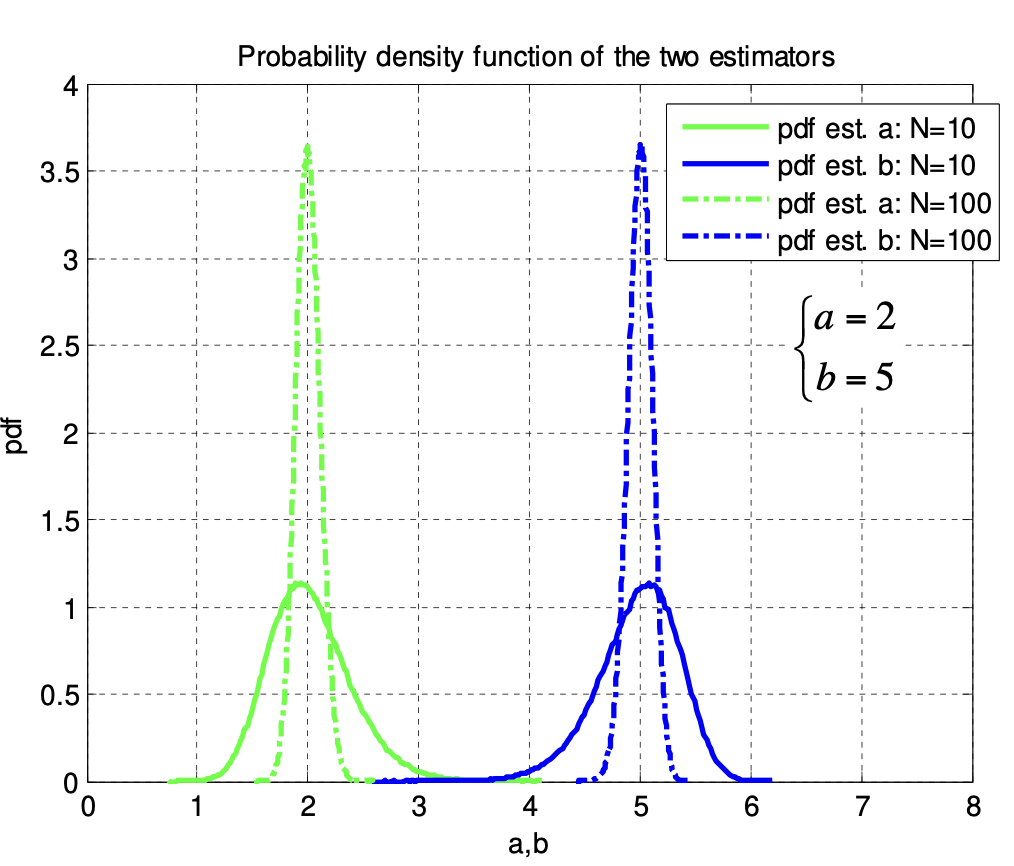
\includegraphics[width=0.75\linewidth]{Image/pdf 4/2.Example_2.png}
    \label{fig:placeholder}
\end{figure}
    \item \textbf{Example 3} Estimates the two parameters \(\eta\) e \(\sigma^2\) of a Gaussian pdf, given \(N\) independent or the r.v. \(X\), assumed to be Gaussian distributed.
    $$
    \mathbf{X}_{N \times 1} = \left[ X_1 \quad X_2 \quad \cdots \quad       X_N \right]^T, \quad \left\{ X_i \right\}_{i=1}^N \ \text{IID}
    $$

    $$
    f_{X_i}(x_i) = \frac{1}{\sqrt{2\pi\sigma^2}} \, e^{ -\frac{(x_i-\eta)^2}{2\sigma^2} }
    \rightarrow
    m_1 \triangleq E\left\{ X_i \right\} = \eta, \qquad
    \mu_2 \triangleq \mathrm{var}\left\{ X_i \right\} = \sigma^2
    $$


    \item In this particular case, two unknown parameters \(\eta\) and \(\sigma^2\) coincide with the first two moments of the distribution, mean and variance. Hencem there are no equations to be solved. The \textbf{Sample Mean} and \textbf{Sample Variance} directly provides the MM estimates of parameters \(\eta\) and \(\sigma^2\):
    $$
\hat{\eta}_{MM} = \hat{m}_1 = \frac{1}{N} \sum_{i=1}^N X_i,
\qquad
\hat{\sigma}^2_{MM} = \hat{\mu}_2 = \frac{1}{N} \sum_{i=1}^N ( X_i - \hat{m}_1 )^2
$$

    \noindent The performance of the \textbf{Sample Mean} and \textbf{Sample Variance} have already been derived under the assumption that the \(N\) observed data are IID:
$$
\hat{\eta} = \frac{1}{N} \sum_{i=1}^N X_i
$$

$$
E\left\{ \hat{\eta} \right\} = E\left\{ \frac{1}{N} \sum_{i=1}^N X_i \right\}
= \frac{1}{N} \sum_{i=1}^N E\left\{ X_i \right\}
= \frac{1}{N} \sum_{i=1}^N \eta
= \eta
$$

$$
\mathrm{var}\left\{ \hat{\eta} \right\}
= \mathrm{var}\left\{ \frac{1}{N} \sum_{i=1}^N X_i \right\}
= \frac{1}{N^2} \sum_{i=1}^N \mathrm{var}\left\{ X_i \right\}
= \frac{\sigma^2}{N}
$$


    \noindent The \textbf{Sample Mean} estimator is \textbf{unbiased} and \textbf{consistent}.\\
    \noindent Moreover, since in this case the data Gaussian distributed and the estimator is \textbf{linear}, the Sample Mean is also \textbf{Gaussian} distributed.\\
    \noindent The gaussianity of the \textbf{Sample Mean} estimator is asymptotically (\(N\gg1\)) valid in any case, even if the data are non Gaussian, thanks to the \textbf{Central Limit Theorem}:

    $$
\hat{\eta}^a \in \mathcal{N} \left( \eta, \frac{\sigma^2}{N} \right)
$$
    \noindent As concerning the \textbf{Sample Variance} estimator:
$$
\hat{\sigma}^2 = \frac{1}{N} \sum_{i=1}^N (X_i - \hat{\eta})^2
$$

$$
E\left\{ \hat{\sigma}^2 \right\} 
= E\left\{ \frac{1}{N} \sum_{i=1}^N (X_i - \hat{\eta})^2 \right\}
= \left( 1 - \frac{1}{N} \right)\sigma^2
\rightarrow
b\left\{ \hat{\sigma}^2 \right\}
= E\left\{ \sigma^2 - \hat{\sigma}^2 \right\}
= \frac{\sigma^2}{N}
$$
    The estimator is \textbf{biased} but \textbf{aymptotically unbiased}. \vspace*{0.5em}
    \item  \textbf{Assumption}: the observed data \{\(X_i\)\} are IID.\\
    \noindent \textbf{Mean value} of the Sample Variance:
$$
\hat{\sigma}^2 = \frac{1}{N} \sum_{i=1}^N (X_i - \hat{\eta})^2
= \frac{1}{N} \sum_{i=1}^N X_i^2 - 2 \frac{1}{N} \sum_{i=1}^N X_i \hat{\eta} + \frac{1}{N} \sum_{i=1}^N \hat{\eta}^2
= \frac{1}{N} \sum_{i=1}^N X_i^2 - \hat{\eta}^2
$$

$$
E\{ \hat{\sigma}^2 \}
= E\left\{ \frac{1}{N} \sum_{i=1}^N X_i^2 - \hat{\eta}^2 \right\}
= E\left\{ \frac{1}{N} \sum_{i=1}^N X_i^2 \right\} - E\left\{ \hat{\eta}^2 \right\}
$$

$$
= \frac{1}{N} \sum_{i=1}^N E\{ X_i^2 \}
- \left( \mathrm{var}\{\hat{\eta}\} + (E\{ \hat{\eta} \})^2 \right)
= \frac{1}{N} \sum_{i=1}^N (\sigma^2 + \eta^2)
- \left( \frac{\sigma^2}{N} + \eta^2 \right)
$$

$$
= \sigma^2 - \frac{\sigma^2}{N}
= \left( 1 - \frac{1}{N} \right) \sigma^2
$$


    \noindent As concerning the \textbf{variance} of the Sample variance for IID data:\\
$$
\mathrm{var}\left\{ \hat{\sigma}^2 \right\}
= \frac{ \mu_X(4) - \sigma^4 }{N}
- \frac{ 2 \left( \mu_X(4) - 2\sigma^4 \right) }{N^2}
+ \frac{ \mu_X(4) - 3\sigma^4 }{N^3}
$$

$$
\text{where} \quad \mu_X(4) \triangleq E\left\{ (X_i - \eta)^4 \right\}
$$

    \item If the data are \underline{IID Gaussian distributed}:
    $$
\mu_X(4) = 3\sigma^4
\implies
\mathrm{var}\left\{\hat{\sigma}^2 \right\}
= \frac{2\sigma^4}{N} - \frac{2\sigma^4}{N^2}
= \frac{2\sigma^4}{N} \left( 1 - \frac{1}{N} \right)
$$
    \noindent When the data are IID Gaussian, we can also derive the exact pdf of the estimator \textbf{Sample Variance}, using the following known result:

    $$
\text{Given} \quad
S \triangleq \sum_{i=1}^{N} \left( \frac{X_i - \hat{\eta}}{\sigma} \right)^2
\qquad
\text{where} \quad
\hat{\eta} \triangleq \frac{1}{N} \sum_{k=1}^{N} X_k
$$
    If the \(\{X_i\}\) are IID Gaussian, then \(S\) is a \textbf{central CHI-Squared} distributed r.v. with \(N-1\) degrees of freedom. Its \textbf{mean} value and \textbf{variance} are given by:
$$
\mathrm{var}\left\{ \hat{\sigma}^2 \right\}
= \mathrm{var}\left\{ \frac{\sigma^2}{N} S \right\}
= \frac{\sigma^4}{N^2} \mathrm{var}\{ S \}
= \frac{2(N-1)}{N^2} \sigma^4
= \frac{2\sigma^4}{N} \left( 1-\frac{1}{N} \right)
$$

$$
MSE\left\{ \hat{\sigma}^2 \right\}
= b^2\left\{ \hat{\sigma}^2 \right\} + \mathrm{var}\left\{ \hat{\sigma}^2 \right\}
= \left( \frac{\sigma^2}{N} \right)^2
+ \frac{2(N-1)}{N^2} \sigma^4
= \frac{2\sigma^4}{N} \left( 1 - \frac{1}{2N} \right)
$$



    \item For larger sample size \(N\gg1\): \[
    MSE\{\hat{\sigma}^2\}\approx\frac{2\sigma^4}{N}
    \]
    \item For the Central-Limit Theorem, we have that the Sample Variance is asymptotically (\(N\gg1\)) Gaussian distributed with the mean and variance derived above:
    \[
    \hat{\sigma}^2 \overset{a}{\in} \mathcal{N} \left( \sigma^2,\, \frac{2 \sigma^4}{N} \right)
    \]
    \item The exact pdf of the Sample Variance estimator is immediately obtained from the pdf of \(S\), which is known in the scientific literature:
\[
\hat{\sigma}^2 = \frac{1}{N} \sum_{i=1}^{N} (X_i - \hat{\eta})^2 = \frac{\sigma^2}{N} S 
\;\;\; \rightarrow \;\;\;
f_{\hat{\sigma}^2}(\hat{\sigma}^2) = \frac{N}{\sigma^2} f_{S}\left( \frac{N}{\sigma^2} \hat{\sigma}^2 \right)
\]
    \item The pdf of a \textbf{central Chi-Squared} r.v. \(S\) with \(N-1\) degrees of freedom is:
\[
\hat{\sigma}^2 = \frac{1}{N} \sum_{i=1}^{N} (X_i - \hat{\eta})^2 = \frac{\sigma^2}{N} S 
\;\;\; \rightarrow \;\;\;
f_{\hat{\sigma}^2}(\hat{\sigma}^2) = \frac{N}{\sigma^2} f_{S}\left( \frac{N}{\sigma^2} \hat{\sigma}^2 \right)
\]
    SERIES OF GRAPH WHERE: MORE N => Sample Variance pdf is similar to the Gaussian Approximation.
    \begin{figure}[H]
        \centering
        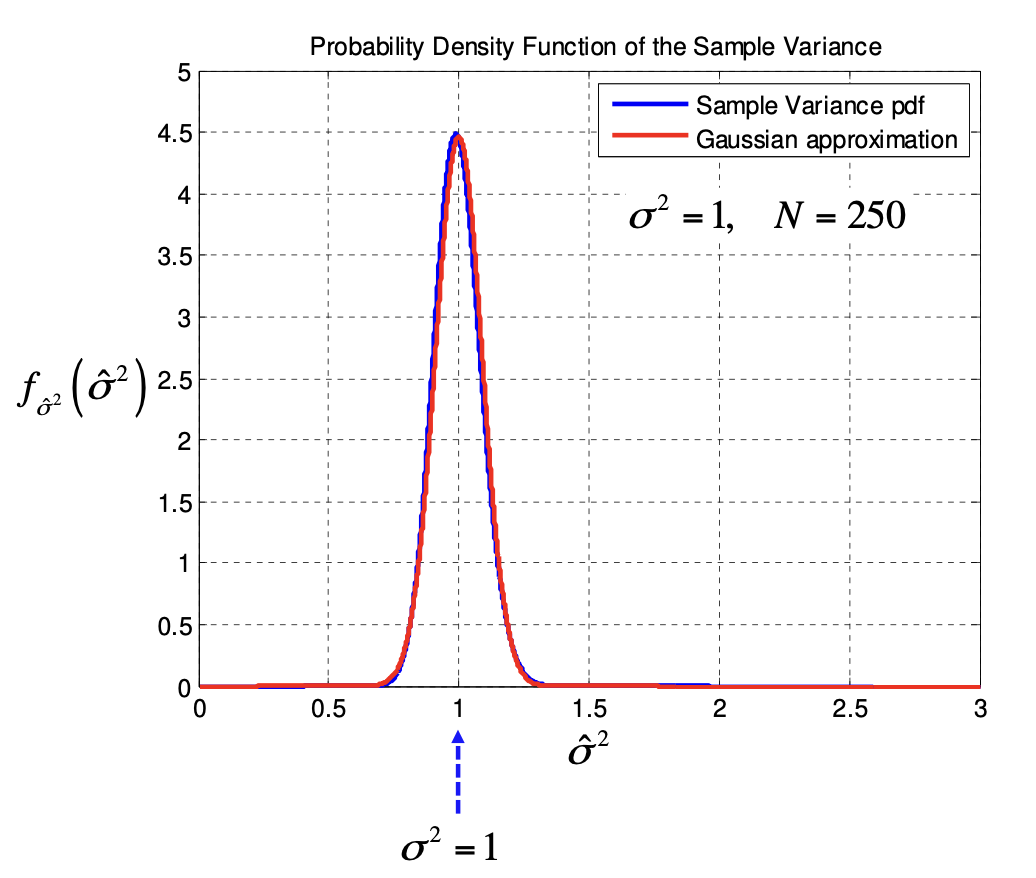
\includegraphics[width=0.75\linewidth]{Image/pdf 4/3.Graph.png}
        \label{fig:placeholder}
    \end{figure}
    \item \textbf{Real high-resolution sea clutter data}.
    \[
    \text{Clutter amplitude: } R=|X_I+jX_Q|
    \]
    \item We want to find the model that "best" matches the observed data.
    \item We hypothesize different parametric models, estimate their parameters from the data and then plot the various pdf's calculated by using the estimated values of the unknown parameters.
    \item Finally, we plot the data \textbf{histogram}, that represents a non model-based estimator of the data pdf.
\begin{figure}[H]
    \centering
    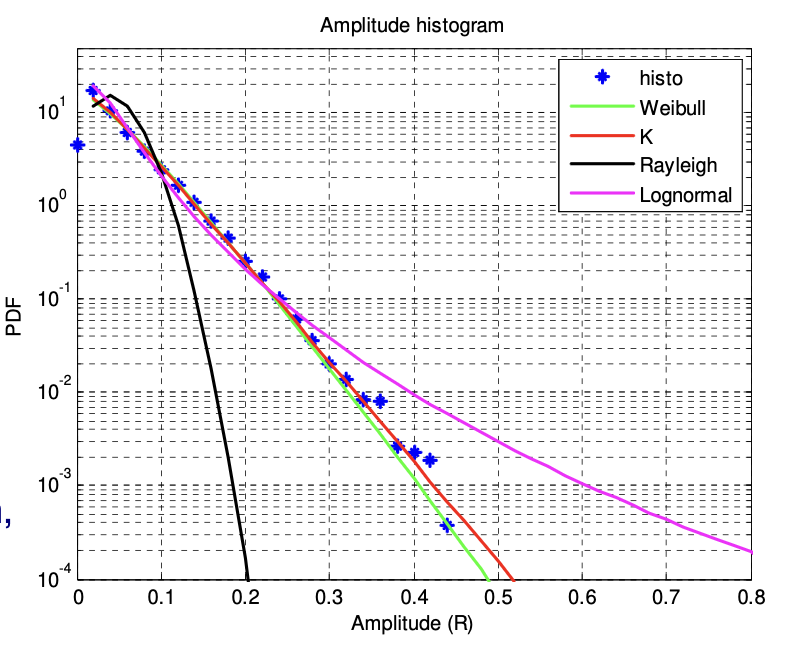
\includegraphics[width=0.75\linewidth]{Image/pdf 4/4.Histogram.png}

    \label{fig:placeholder}
\end{figure}
    \[
    f_R(\mathbf{r}; \boldsymbol{\theta}) \;\rightarrow\; \hat{\boldsymbol{\theta}}_{MM} \;\rightarrow\; \hat{f}_R(r) = f_R\left(r; \hat{\boldsymbol{\theta}}_{MM}\right)
    \]
    \item Finally, we select the one which provides the best fit.
    \item The \textbf{MM} is fairly simple and yields \textbf{consistent} estimator (under very weak assumptions), though these estimators are often \textbf{biased}.
    \item In some respects, when estimating parameters of a known family of pdf's, this method was superseded by \textbf{Fisher's method} of \textbf{Maximum likelihood(ML)}, because ML estimators have higher probability of being close to the quantities to be estimaeted and are more often unbiased.
    \item However, in some cases the likelihood equations may be intractable without computers and the ML estimators cannot be found in closed-form, whereas the MM estimators can be quickly and easily calculated by hand, provided we are able to solve the equation:\[
    \mu = \textbf{h}(\theta)
    \]
    \item MM estimates may be used as the first approximation to the solutions of the likelihood equations, and successive improved approximations may then be found by the Newton-Raphson method. In this way the MM estimates can help in finding the ML estimates.
    \item In some cases, infrequent with large samples but not so infrequent with small samples, the MM estimates are outside of the parameter space. This problem never arises in the ML estimators.
    \item MM estimates by the method of moments are not necessarily \textbf{sufficient statistics}, i.e. they sometimes fail to take into account all relevant information in the sample.
    \item Let us now introduce the \textbf{Maximum Likelihood (ML) method}.
\end{itemize}
\subsection{The Maximum Likelihood (ML) Estimate}
\begin{itemize}
    \item Calculate now the probability that the r.v. \(X\) assumes a value that belong to the interval centered around the observed value \(x\) of infinitesimal length \(\Delta\): \(X\in[x-\Delta/2,x+\Delta/2]\), for each of the three values of \(\theta\):
    \[
    f_X(x; \theta) \rightarrow P_{i} \triangleq \int_{x - \Delta/2}^{x + \Delta/2} f_X(\alpha; \theta_{i})\, d\alpha = f_X(x; \theta_{i}) \Delta
    \]
    \item The idea of the ML method is to choose the value of \(\theta\) which maximized the probability \(P_i\) of observing a value of \(X\in[x-\Delta/2,x+\Delta/2]\):
    \[
    \hat{\theta} = \arg\max_{\theta \in \{\theta_1, \theta_2, \theta_3\}} P_i = \arg\max_{\theta \in \{\theta_1, \theta_2, \theta_3\}} f_X(x;\theta) \Delta = \arg\max_{\theta \in \{\theta_1, \theta_2, \theta_3\}} f_X(x;\theta)
    \]
    \item In the previous example, where \(x=3\), the ML criterion bring us to select \(\theta=2\) as the most likely value, i.e. the value that maximizes the likelihood of observing that specific value of x. In this case the ML estimate of \(\theta\) would be 2.
    \item Hence, the ML estimates is obtained by looking for the value of \(\theta\) which maximizes the pdf of the observed data, given the observed data \(X=x\):
    \[
    \hat{\theta}_{ML}=\underset{\theta}{\text{arg}\max} f_X(x;\theta)
    \]
    \item In general, the parameter \(\theta\) is continuos, i.e. \(\theta\in\mathcal{R}\).
    \item The generalization to the case of \(N\) observed data is immediate:
    \[
    \hat{\theta}_{ML}=\underset{\theta}{\text{arg}\max}f_X(\textbf{x};\theta)
    \]
    \item It is worth observing that we should look at the pdf no more as a function of the data vector \textbf{x}, but as a function of the unknown parameter \(\theta\).
    \item When seen as a function of the unknown parameter \(\theta\), the pdf of the observed data is called \textbf{Likelihood Function(LF)}.
    \item Sometimes, we prefer to operate on the natural logarithm of the likelihood function, the \textbf{Log-Likelihood Function(LLF)}:
    \[
    L(\theta)\triangleq f_X(\mathbf{x};\theta)\qquad\ln L(\theta)\triangleq\ln f_X(\mathbf{x};\theta)
    \]
    \item The estimator that is obtained by maximizing the likelihood function is called the \textbf{Maximum Likelihood (ML) estimator}:
    \[
    \hat{\theta}_{ML} = \arg\max_{\theta} f_X(\mathbf{x}; \theta) = \arg\max_{\theta} L(\theta) = \arg\max_{\theta} \ln L(\theta)
    \]
    \item Clearly, the estimate is a function of the observed data \textbf{x}, even if not explicitly written.
    \item In general, any time that the \textbf{LF} is continuous and differentiable in the definition inteval of the parameter \(\theta\) to be estimated and the maximum is not on the border of the definition interval, the ML estimate can be obtained by solving the following equation (the \textbf{likelihood equation}):\[
    \left. \frac{\partial L(\theta)}{\partial \theta} \right|_{\theta = \hat{\theta}_{ML}} = 0, \quad \text{or} \quad \left. \frac{\partial \ln L(\theta)}{\partial \theta} \right|_{\theta = \hat{\theta}_{ML}} = 0
    \]
    \item When we have to estimate \textbf{multiple parameters}, e.g. \(P\) parameters, we must derive the LF with respect to all the parameters and the set the derivative equal to zero, so obtaining a system of \(P\) equations in \(P\) unknowns:
    \item In general, we cannot claim that the ML estimate is the optimal one, i.e. the one with the minimum MSE, since, as we have seen, \underline{an optimal estimator does not exist} (for deterministic parameters). However, the \textbf{ML estimate} enjoys the following \textbf{properties}:
    \[
    \boldsymbol{\theta} = 
    \begin{bmatrix}
    \theta_1 \quad \theta_2 \quad \cdots \quad \theta_P
    \end{bmatrix}^T
    \quad \rightarrow \quad
    \left. 
    \frac{\partial \ln L(\boldsymbol{\theta})}{\partial \theta_i}
    \right|_{\boldsymbol{\theta} = \hat{\boldsymbol{\theta}}_{ML}}
    = 0, \quad i=1,2,\ldots,P
    \]
    \begin{itemize}
        \item Asymptotically unbiased;
        \item Consistent;
        \item Asymptotically efficient (the one with the lowest possibile MSE);
        \item Asymptotically Gaussian distributed;
        \item There is no guarantee that the ML estimator is efficient, but if an efficient estimator exists, it is the ML estimator.
        \item The concept of \textbf{efficiency} is related to the definition of the so-called \textbf{Cramèr-Rao lower bound (CRB)}, that we will introduce in the following.
    \end{itemize}
    \item \textbf{EXAMPLE}: Derive the ML estimate of the parameters \(\eta\) and \(\sigma^2\) of a Gaussian r.v. \(X\), given \(N\) independent realizations of \(X\):
    \[
    \mathbf{X}_{N \times 1} = \begin{bmatrix}
    X_1 \quad X_2 \quad \cdots \quad X_N
    \end{bmatrix}^T,
    \quad \left\{ X_i \right\}_{i=1}^N \quad \text{IID}
    \]

    \[
    f_{X_i}(x_i) = \frac{1}{\sqrt{2\pi \sigma^2}} e^{- \frac{(x_i - \eta)^2}{2 \sigma^2}}
    \quad \rightarrow \quad
    m_1 = E\{X_i\} = \eta, \quad \mu_2 = \mathrm{var}\{X_i\} = \sigma^2
    \]

    \[
    f_{\mathbf{X}}(\mathbf{x}; \eta, \sigma^2) = \prod_{i=1}^{N} f_{X_i}(x_i; \eta, \sigma^2) =
    \prod_{i=1}^N \frac{1}{\sqrt{2\pi \sigma^2}} e^{- \frac{(x_i - \eta)^2}{2 \sigma^2}}
    = (2\pi \sigma^2)^{-\frac{N}{2}} \exp \left( -\frac{1}{2\sigma^2} \sum_{i=1}^N (x_i - \eta)^2 \right)
    \]

    \[
    \ln L(\eta, \sigma^2) = \ln f_{\mathbf{X}}(\mathbf{x}; \eta, \sigma^2) =
    - \frac{N}{2} \ln (2\pi \sigma^2) - \frac{1}{2\sigma^2} \sum_{i=1}^N (x_i - \eta)^2
    \]
    \item \textbf{Case study 1}: \(\eta\) unknown and \(\sigma^2\) known (>0):
    \[
    \frac{d \ln L(\eta, \sigma^2)}{d \eta}
    = \frac{d \ln f_{\mathbf{x}}(\mathbf{x}; \eta, \sigma^2)}{d\eta}
    = \frac{1}{\sigma^2} \sum_{i=1}^{N} (x_i - \eta)
    = \frac{1}{\sigma^2} \left( \sum_{i=1}^{N} x_i - N\eta \right)
    \]

    \[
    \frac{d \ln L(\eta, \sigma^2)}{d \eta} = 0
    \quad \rightarrow \quad
    \sum_{i=1}^{N} x_i - N\eta = 0
    \quad \rightarrow \quad
    \eta = \frac{1}{N} \sum_{i=1}^{N} x_i
    \]

    \[
    \hat{\eta}_{ML} = \frac{1}{N} \sum_{i=1}^{N} X_i
    \quad \text{ \small{(tre metodi diversi che coincidono)} }
    \]
    \item The ML estimate of the parameter \(\eta\) (the mean value) of a Guassian r.v. \(X\), when the variance \(\sigma^2\) is a priori known, coincides with the \textbf{Sample Mean}, that is also the estimator we obtained by the \textbf{Method of Moments}.
    \item \textbf{Case study 2}: \(\eta\) known and \(\sigma^2\) unknown (>0):
\[
\frac{d \ln L(\eta, \sigma^2)}{d \sigma^2}
= \frac{d \ln f_{\mathbf{x}}(\mathbf{x}; \eta, \sigma^2)}{d \sigma^2}
= -\frac{N}{2} \cdot \frac{1}{\sigma^2}
+ \frac{1}{2 (\sigma^2)^2} \sum_{i=1}^N (x_i - \eta)^2
\]

\[
\frac{d \ln L(\eta, \sigma^2)}{d \sigma^2} = 0
\quad \rightarrow \quad
-\frac{N}{2} \cdot \frac{1}{\sigma^2} + \frac{1}{2 (\sigma^2)^2} \sum_{i=1}^N (x_i - \eta)^2 = 0
\quad \rightarrow \quad
\sigma^2 = \frac{1}{N} \sum_{i=1}^N (x_i - \eta)^2
\]

\[
\hat{\sigma}^2_{ML} = \frac{1}{N} \sum_{i=1}^{N} (X_i - \eta)^2
\]

\[
E\left\{ \hat{\sigma}^2_{ML} \right\}
= E\left\{ \frac{1}{N} \sum_{i=1}^{N} (X_i - \eta)^2 \right\}
= \frac{1}{N} \sum_{i=1}^{N} E\left\{ (X_i - \eta)^2 \right\}
= \sigma^2
\]
    
    \item \textbf{IMPORTANT}: The ML estiamte of the variance \(\sigma^2\) when the mean \(\eta\) is a priori known is unbiased.
    \[
MSE\left\{\hat{\sigma}^2_{ML}\right\}
= \text{var}\left\{\hat{\sigma}^2_{ML}\right\} + \left( b\left\{\hat{\sigma}^2_{ML}\right\} \right)^2
= \text{var}\left\{\hat{\sigma}^2_{ML}\right\}
\]

\[
= \text{var}\left\{
\frac{1}{N} \sum_{i=1}^{N} (X_i - \eta)^2
\right\}
= \frac{1}{N^2} \sum_{i=1}^{N} \text{var}\left\{ (X_i - \eta)^2 \right\}
\]

\[
= \frac{1}{N} \text{var}\left\{ (X_i - \eta)^2 \right\}
\]

\[
= \frac{1}{N} \left[
E\left\{ (X_i - \eta)^4 \right\}
- \left( E\left\{ (X_i - \eta)^2 \right\} \right)^2
\right]
\]

\[
= \frac{\mu_X(4) - (\sigma^2)^2}{N}
= \frac{3\sigma^4 - (\sigma^2)^2}{N}
= \frac{2\sigma^4}{N}
\]
    \item It is worth observing that this value coincides with the asymptotical (\(N\gg 1\)) value of the MSe of the Sample Variance estimator (obtained under the assumption that also the mean is unknown).
    \item \textbf{Case study 3}: \(\eta\) and \(\sigma^2\) both unknowns (\(\sigma^2>0\)).
    \[
\begin{cases}
\displaystyle
\frac{d \ln f_{X}(\mathbf{x}; \eta, \sigma^2)}{d\eta}
= \frac{1}{\sigma^2} \left( \sum_{i=1}^N x_i - N \eta \right) = 0 \\[8pt]
\displaystyle
\frac{d \ln f_{X}(\mathbf{x}; \eta, \sigma^2)}{d\sigma^2}
= -\frac{N}{2} \cdot \frac{1}{\sigma^2}
+ \frac{1}{2\sigma^4} \sum_{i=1}^N (x_i - \eta)^2 = 0
\end{cases}
\]
    \item We solve the first equation w.r.t \(\eta\) and we insert it in the second equation:
    \[
    \begin{cases}
    \displaystyle
    \eta = \frac{1}{N} \sum_{i=1}^{N} x_i \\[8pt]
    \displaystyle
    \sigma^2 = \frac{1}{N} \sum_{i=1}^{N} \left( x_i - \frac{1}{N} \sum_{k=1}^{N} x_k \right)^2
    \end{cases}
    \]
    \item The joint \textbf{ML estimators of mean and variance of a Gaussian distribution} are given by the \textbf{Sample Mean} and the \textbf{Sample Variance}, previously derived, also via the Method of Moments:
    \[
\hat{\eta}_{ML} = \frac{1}{N} \sum_{i=1}^{N} X_i
\]

\[
\hat{\sigma}^2_{ML} = \frac{1}{N} \sum_{i=1}^{N} \left( x_i - \frac{1}{N} \sum_{k=1}^{N} x_k \right)^2
= \frac{1}{N} \sum_{i=1}^{N} (x_i - \hat{\eta}_{ML})^2
\]

\[
MSE\left\{ \hat{\eta}_{ML} \right\} = \frac{\sigma^2}{N},
\qquad
MSE\left\{ \hat{\sigma}^2_{ML} \right\} \simeq \frac{2\sigma^4}{N} \left( 1 - \frac{1}{2N} \right)
\quad \xrightarrow{N \gg 1} \quad \frac{2\sigma^4}{N}
\]
    \item \textbf{EXAMPLE}: We have a random variable \(X\) having uniform distribution between 0 and \(\theta\), where \(\theta>0\). We want to derive the ML and MM estiamtors of the parameter \(\theta\), given \(N\) independent realizations of \(X\) and the to compare their performance:
    \[
    f_X(x;\theta) = \frac{1}{\theta} \, \mathrm{rect}\left(\frac{x - \theta/2}{\theta}\right) = 
    \begin{cases}
    \frac{1}{\theta}, & 0 \leq x \leq \theta \\
    0, & \textit{otherwise}
    \end{cases}
    \]
    \begin{figure}[H]
        \centering
        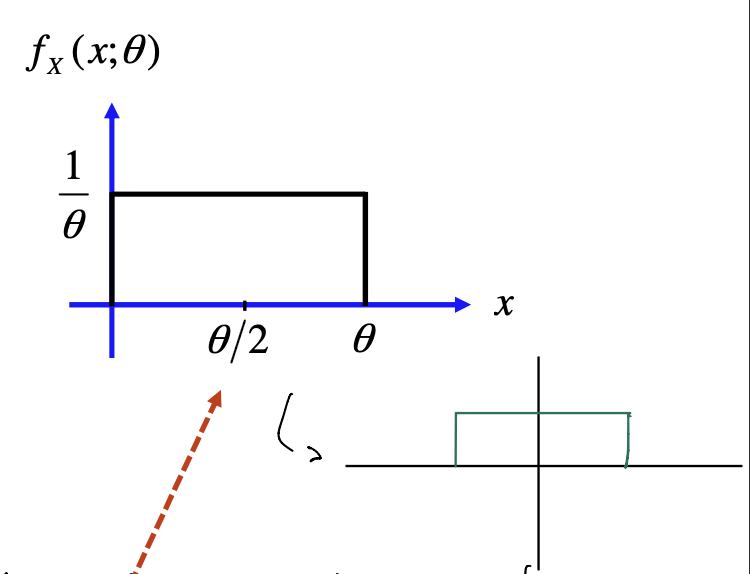
\includegraphics[width=0.5\linewidth]{Image/pdf 4/5.Example 1.png}
        \label{fig:placeholder}
    \end{figure}
    \begin{itemize}
        \item Let us derive first the \textbf{MM estimator}.
        The first step is to calculate the mean of \(X\):
        \[
        m_1 = E\{X\} = \frac{\theta}{2} \qquad \text{(the mean value is the symmetry point of the pdf)}
        \]
        By inverting this relationship we get:
        \[
\theta = 2m_1 \;\;\;\Rightarrow\;\;\;
\hat{\theta}_{MM}(\mathbf{x}) = 2\hat{m}_1 = \frac{2}{N} \sum_{i=1}^{N} X_i
\]
        Calculation of the \textbf{bias}:
        \[
E\left\{ \hat{\theta}_{MM}(\mathbf{x}) \right\}
= E\left\{ \frac{2}{N} \sum_{i=1}^{N} X_i \right\}
= \frac{2}{N} \sum_{i=1}^{N} E\{X_i\}
= \frac{2}{N} \sum_{i=1}^{N} \frac{\theta}{2}
= \theta
\]
        The MM estimator is \textbf{unbiased}. Hence, the MSE coincides with the variance:
        \[
MSE\left\{ \hat{\theta}_{MM}(\mathbf{x}) \right\}
= \mathrm{var}\left\{\hat{\theta}_{MM}(\mathbf{x})\right\}
= \mathrm{var} \left\{ \frac{2}{N} \sum_{i=1}^{N} X_i \right\}
= \frac{4}{N^2} \sum_{i=1}^{N} \mathrm{var}\{X_i\}
\]

\[
= \frac{4}{N^2} \cdot N \cdot \frac{\theta^2}{12}
= \frac{\theta^2}{3N}
\qquad \longrightarrow \text{è consistente}
\]
        \item Let us now derive the \textbf{ML estimator}. The first step is to understand which is the behavior of the likelihood function (LF).
        Let us start from the simplest case of \(N=1\):
        \[
        L(\theta) = f_X(x_1; \theta) =
        \begin{cases}
        1/\theta, & 0 \leq x_1 \leq \theta \\
        0,        & \textit{otherwise}
        \end{cases}
        \]
        \begin{figure}[H]
            \centering
            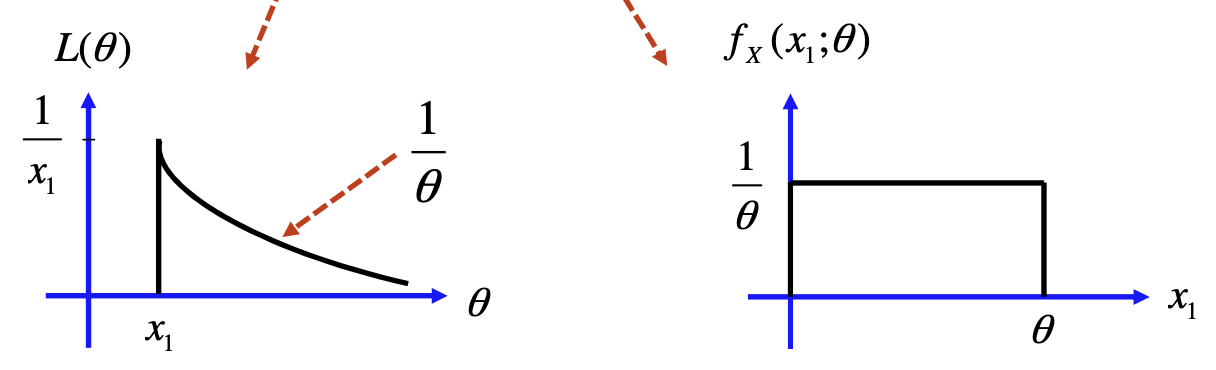
\includegraphics[width=0.75\linewidth]{Image/pdf 4/6.Example 2.png}
            \label{fig:placeholder}
        \end{figure}
        For \(N=2\), exploiting the independence of the observed data:
\[
L(\theta) = f_X(\mathbf{x}; \theta) = \prod_{i=1}^{N} f_X(x_i; \theta)
\]

\[
\begin{aligned}
N=2: \quad
f_X(x_1; \theta) f_X(x_2; \theta) &= \frac{1}{\theta} \, \mathrm{rect}\left( \frac{x_1 - \theta/2}{\theta} \right) \cdot
\frac{1}{\theta} \, \mathrm{rect}\left( \frac{x_2 - \theta/2}{\theta} \right) \\[10pt]
&=
\begin{cases}
1/\theta^2, & 0 \leq x_1 \leq \theta, \; 0 \leq x_2 \leq \theta \\
0, & \textit{otherwise}
\end{cases}
\\[10pt]
&=
\begin{cases}
1/\theta^2, & 0 \leq \max\{x_1, x_2\} \leq \theta \\
0, & \textit{otherwise}
\end{cases}
\end{aligned}
\]

\[
L(\theta) = \frac{1}{\left( \max\{x_1, x_2\} \right)^2}
\quad \text{ per il valore massimo}
\]
        For a generic \(N\):
        \[
L(\theta) = f_X(\mathbf{x}; \theta) = \prod_{i=1}^N f_X(x_i; \theta)
\]

\[
= \prod_{i=1}^N \left[ \frac{1}{\theta} \; \mathrm{rect}\left( \frac{x_i - \theta/2}{\theta} \right) \right]
= \frac{1}{\theta^N} \prod_{i=1}^N \mathrm{rect}\left( \frac{x_i - \theta/2}{\theta} \right)
\]

\[
=
\begin{cases}
1/\theta^N, & 0 \leq x_1 \leq \theta,\, 0 \leq x_2 \leq \theta,\, \cdots,\, 0 \leq x_N \leq \theta \\
0, & \textit{otherwise}
\end{cases}
\]

\[
=
\begin{cases}
1/\theta^N, & 0 \leq \max\{x_1, x_2, \dots, x_N\} \leq \theta \\
0, & \textit{otherwise}
\end{cases}
\]

\[
\max\{x_i\} \triangleq \max\{x_1, x_2, \cdots, x_N\}
\]
    \item In this cae, the likehood function is not continuous and differentiable everywhere in definition interval of the parameter \(\theta\), that is \(\theta\in(0,+\infty)\), in particular, as we will see, it is not continuous and differentiable in the maximum. Hence, the ML estimate cannot be obtained by solving the \textbf{likelihood equation}, but it must be obtained by looking directly for the value of \(\theta\) for which \(L(\theta)\) is maximum.
    \item In our case, by inspection of the previous figures we immediately obtain:
$$
\hat{\theta}_{ML} = \arg\max_{\theta} L(\theta) = \max \left\{ x_1, x_2, \cdots, x_N \right\}
$$

    \item ML estimation requires ordering of the data \(\textbf{Ordered statics, OS}\).
    \item For performance analysis of the ML estimator, we have to derive the \textbf{bias} and the \textbf{MSE}.
    \item To this purpose, we need to derive the \textbf{pdf} of the estimator and then its \textbf{mean} value and \textbf{variance}.
    \item Let us derive the pdf of the ML estimator by applying the method of the \textbf{cumulative distribution function (cdf)}:
    $$
    X_M \triangleq \hat{\theta}_{ML} = \max \left\{ X_1, X_2, \cdots, X_N \right\}
    $$

    $$
    f_{X_M}(x_M) = \frac{dF_{X_M}(x_M)}{dx_M}, \qquad \text{where} \quad F_{X_M}(x_M) \triangleq \Pr\left\{ X_M \leq x_M \right\}
    $$
    \item The maximum is lower than \(x_M\) only if all the observed data are lower than \(x_M\):
    $$
F_{X_M}(x_M) \triangleq \Pr\left\{ X_M \leq x_M \right\} = \Pr\left\{ \max\{ X_1, X_2, \cdots, X_N \} \leq x_M \right\}
$$
$$
= \Pr\left\{ X_1 \leq x_M,\, X_2 \leq x_M,\, \cdots,\, X_N \leq x_M \right\}
$$
$$
= \Pr\left\{ X_1 \leq x_M \right\} \Pr\left\{ X_2 \leq x_M \right\} \cdots \Pr\left\{ X_N \leq x_M \right\}
$$
    \item Where we exploited the assumption that the observed data are \underline{independent}.
    \item If we now exploit also the assumption that the data are identically distributed, i.e. they have the same pdf and so the same cdf:
    $$
F_{X_M}(x_M) = \Pr\{X_1 \leq x_M\} \Pr\{X_2 \leq x_M\} \cdots \Pr\{X_N \leq x_M\}
$$
$$
= \prod_{i=1}^{N} \Pr\{X_i \leq x_M\} = \prod_{i=1}^{N} F_X(x_M) = \left[F_X(x_M)\right]^N
$$
    \item Where the cdf of \(X\) is given:
$$
F_X(x) = \int_{-\infty}^{x} f_X(\alpha) d\alpha = \frac{1}{\theta} \int_{-\infty}^{x} \text{rect}\left(\frac{\alpha - \theta/2}{\theta}\right) d\alpha
$$
$$
= 
\begin{cases}
0, & x < 0 \\
\frac{x}{\theta}, & 0 \leq x \leq \theta \\
1, & x > \theta
\end{cases}
$$


    \item Hence, the cdf of the ML estimate is given by:
    $$
    F_{X_M}(x_M) = \left[ F_X(x_M) \right]^N =
    \begin{cases}
    0, & x_M < 0 \\
    \left( \dfrac{x_M}{\theta} \right)^N, & 0 \leq x_M \leq \theta \\
    1, & x_M > \theta
    \end{cases}
    $$
    \item Finally, the pdf of the ML estimate is obtained by calculating the derivative:
    $$
    f_{X_M}(x_M) = \frac{d F_{X_M}(x_M)}{dx_M} = \frac{d \left[ F_X(x_M) \right]^N }{dx_M} = N \left[ F_X(x_M) \right]^{N-1} f_X(x_M)
    $$

    $$
    =
    \begin{cases}
    \dfrac{N}{\theta} \left(\dfrac{x_M}{\theta}\right)^{N-1}, & 0 \leq x_M \leq \theta \\
    0, & \text{otherwise}
    \end{cases}
    = \frac{N}{\theta} \left(\frac{x_M}{\theta}\right)^{N-1} \text{rect} \left( \frac{x_M - \theta/2}{\theta} \right)
    $$
    
    \begin{figure}[H]
        \centering
        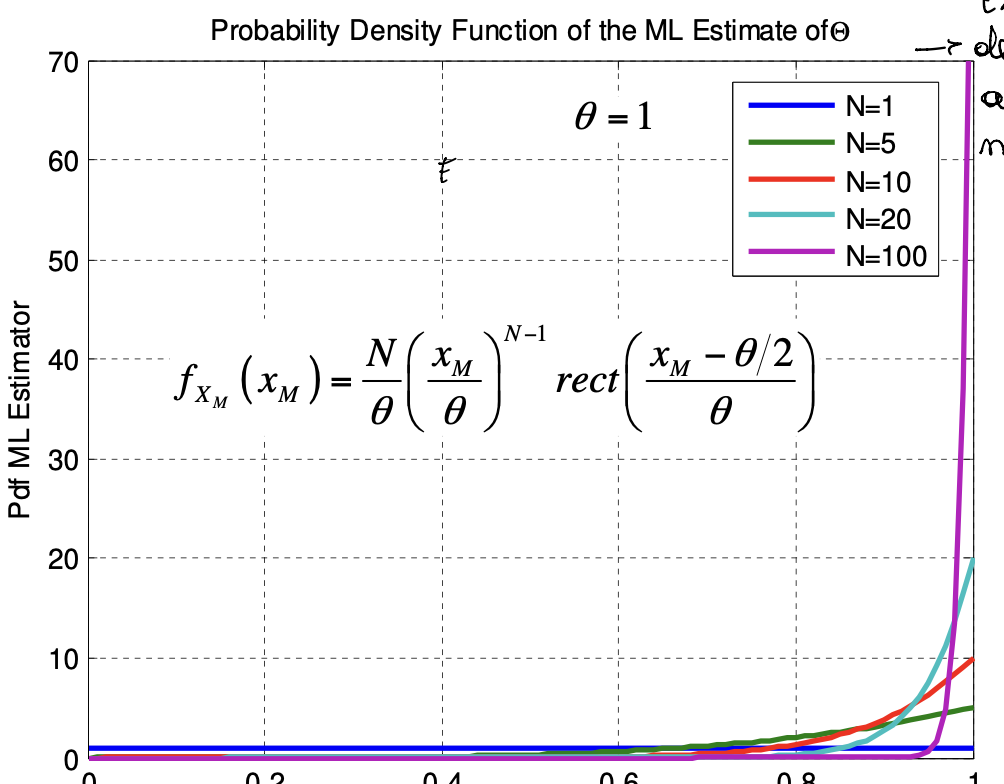
\includegraphics[width=0.5\linewidth]{Image/pdf 4/7.Graph.png}
        \label{fig:placeholder}
    \end{figure}
    \item We can now calculate \textbf{mean} and \textbf{variance} of the ML estimate:
    $$
\text{pdf of } \hat{\theta}_{ML}:\quad f_{X_M}(x_M)=\frac{N}{\theta} \left(\frac{x_M}{\theta}\right)^{N-1} \text{rect}\left(\frac{x_M-\theta/2}{\theta}\right)
$$

$$
E\{\hat{\theta}_{ML}\} = \int_{-\infty}^{+\infty} x_M f_{X_M}(x_M) dx_M = \frac{N}{\theta^N} \int_0^\theta (x_M)^N dx_M = \frac{N}{\theta^N} \left[ \frac{(x_M)^{N+1}}{N+1} \right]_{x_M=0}^{\theta} = \frac{N\theta}{N+1}
$$

$$
E\{\hat{\theta}^2_{ML}\} = \int_{-\infty}^{+\infty} x_M^2 f_{X_M}(x_M) dx_M = \frac{N}{\theta^N} \int_0^\theta (x_M)^{N+1} dx_M = \frac{N}{\theta^N} \left[ \frac{(x_M)^{N+2}}{N+2} \right]_{x_M=0}^{\theta} = \frac{N\theta^2}{N+2}
$$

$$
\text{var}\{\hat{\theta}_{ML}\} = E\{\hat{\theta}^2_{ML}\} - \left(E\{\hat{\theta}_{ML}\} \right)^2 = \frac{N\theta^2}{N+2} - \left( \frac{N\theta}{N+1} \right)^2 = \frac{N\theta^2}{(N+1)^2(N+2)}
$$

    \item Finally, we derive \textbf{bias} and \textbf{MSE} of the ML estimate:
    $$
    b\left\{ \hat{\theta}_{ML} \right\} = E\left\{ \theta - \hat{\theta}_{ML}       \right\} = \theta - E\left\{ \hat{\theta}_{ML} \right\} = \theta -            \frac{N\theta}{N+1} = \frac{\theta}{N+1} \xrightarrow{N \to \infty} 0
    $$
    \item The estimator is \textbf{biased}, but \textbf{asymptotically unbiased}:
    \[
    \begin{aligned}
    MSE\left\{ \hat{\theta}_{ML}(\mathbf{x}) \right\} &= \left( b\left\{ \hat{\theta}_{ML} \right\} \right)^2 + \mathrm{var}\left\{ \hat{\theta}_{ML} \right\}\\[5pt]
    &= \left( \frac{\theta}{N+1} \right)^2 + \frac{N\theta^2}{(N+1)^2(N+2)}
    \\[5pt]
    &= \frac{2\theta^2}{(N+1)(N+2)} \xrightarrow{N \to \infty} 0
    \end{aligned}
    \]
    \item The estimator is \textbf{consistent}.
    \end{itemize}
  
    \item \textbf{Performance comparison:}
    \begin{itemize}
        \item The MSE of the ML estiamtor goes to zero with the law \(1/N^2\). Instead, the MSE of the MM estiamtor goes to zero with the law \(1/N\). Hence, the ML estimator is much more efficient.
        \item The two MSE's coincide only for \(N=1\).
        $$
MSE \left\{ \hat{\theta}_{ML}(\mathbf{x}) \right\} = \frac{2\theta^2}{(N+1)(N+2)} \approx \frac{2\theta^2}{N^2} \quad \text{for } N \gg 1
$$

$$
MSE \left\{ \hat{\theta}_{MM}(\mathbf{x}) \right\} = \frac{\theta^2}{3N}
$$
\begin{figure}[H]
    \centering
    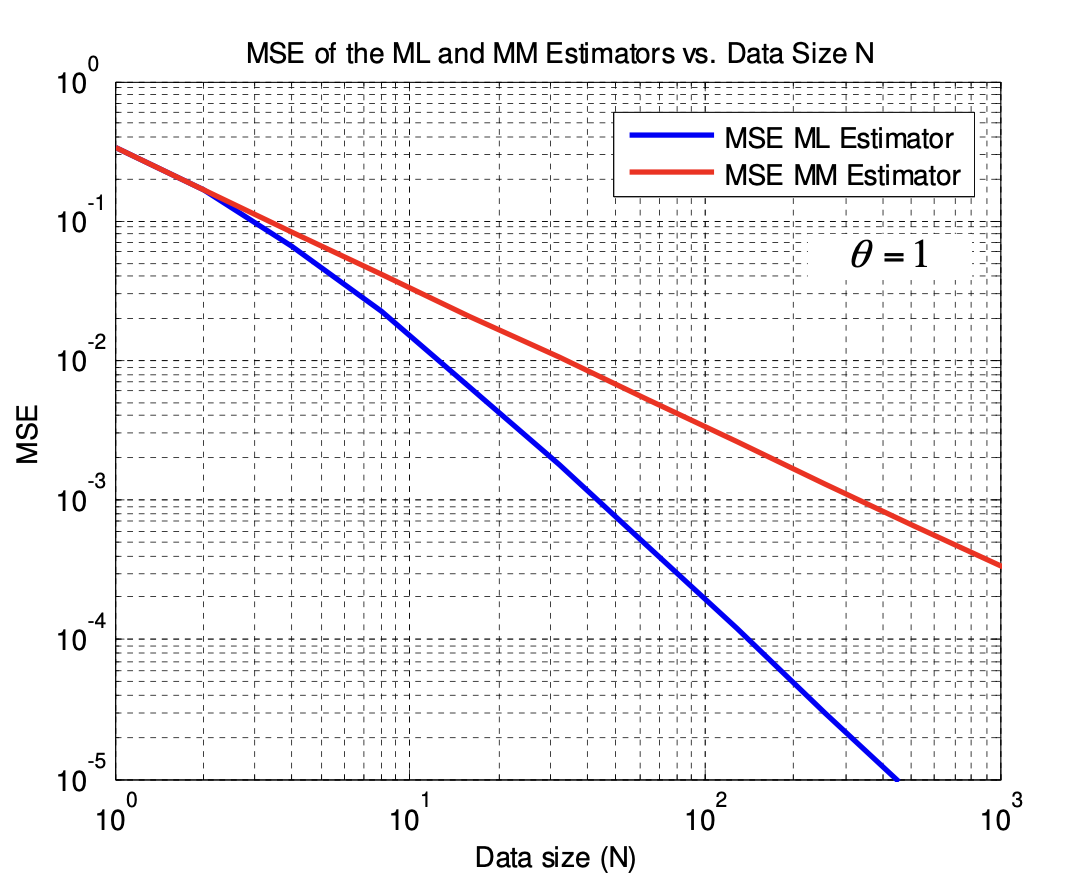
\includegraphics[width=0.5\linewidth]{Image/pdf 4/8.Graph 2 .png}
    \label{fig:placeholder}
\end{figure}
    
    \end{itemize}
    \item \textbf{Comparison in terms of computational complexity}:

    \item The ML estimator is non-linear, it require calculation of the maximum of a set of \(N\)(data ordering).
    \item The MM estimator is linear, hence much more efficient from the point of view of the \textbf{computational complexity}.
    \item The choice between the two depends on the constraints imposed by the specific application: if estimation accuracy is the most important issue, then we should use the ML estimate; if instead it is more important to keep low the computational complexity, we should use the MM estimator.
    \item \textbf{Example}: In a digital communication channel the probability that a symbol is received correctly is \(p\). Assuming that we can observe the result of \(N\) independent trials of the experiment "transmission of a symbol" and check if that symbol has been received correctly of not for any trial, find the \textbf{ML estimator} of \(p\).
    \item Thanks to the fact that the trials are run independently and in the same, condition, the random variable \(K=\{\text{Number of times the symbol has been correctly received}\}\) is a discrete Binomial random variable with parameters \(N\) and \(p\):
    $$
    K \in B(p, N) \quad \text{ "Number of successes"}
    $$
    $$
    p_K(k) = \Pr\{K = k\} = {N \choose k} p^k (1-p)^{N-k}, \quad 0 < p < 1,\quad 0 \leq k \leq N
    $$
    \item Where:
$$
\binom{N}{k} \triangleq \frac{N!}{(N-k)!k!}
$$

$$
E\{K\} = Np, \qquad \mathrm{var}\{K\} = Np(1-p)
$$


    \item To derive the ML estimate of \(p\) we have to find the value of \(p\) which maximizes the likelihood function.
    \item For a discrete random variable, the likehood function is the joint \textbf{mass probability function (mpf)}, seen as a function of the unknown parameter, in this case \(p\):
    $$
    L(p) = p_K(k) = \binom{N}{k} p^k (1-p)^{N-k}, \qquad 0 < p < 1, \ \ 0 \leq k    \leq N
    $$
    \item Since \(L(p)\) is continuous and differentiable w.r.t. \(p\), we derive the ML estimate by solving the \textbf{likelihood function}:
    \[
    \begin{aligned}
    \left. \frac{dL(p)}{dp} \right|&_{p = \hat{p}_{ML}} = 0\\[5pt]
    \frac{dL(p)}{dp} &= \frac{d}{dp} \left\{ \binom{N}{k} p^k (1-p)^{N-k} \right\}\\[5pt]
    &= \binom{N}{k} \, k \, p^{k-1} (1-p)^{N-k} - \binom{N}{k} (N-k) p^k (1-p)^{N-k-1}\\[5pt]
    &= \binom{N}{k} p^{k-1} (1-p)^{N-k-1} \left[ k(1-p) - (N-k)p \right]
    \end{aligned}
    \]
    \item Since the definition interval for \(p\) is \(0<p<1\), we can exclude the trivial solutions \(p=0\) and \(p=1\), so we have :

$$
k(1 - p) - (N - k)p = k - Np = 0 \implies p = \frac{k}{N}
$$

$$
\boxed{\hat{p}_{ML} = \frac{k}{N}}
$$

\item Hence, the estimator \textbf{frequency of occurence} that we have already derived (see the law \textbf{Law of large numbers}) is also the ML estimator. As a consequence, it has all the good properties of the Ml estimators.
    \item \textbf{Bias} and \textbf{MSE}:
$$
E\left\{ \hat{p}_{ML} \right\} = E\left\{ \frac{K}{N} \right\} = \frac{E\{K\}}{N} = \frac{N p}{N} = p \implies b\left\{ \hat{p}_{ML} \right\} = 0
$$


    \item The estimator is \textbf{unbiased}:
$$
\mathrm{var}\left\{ \hat{p}_{ML} \right\} = \mathrm{var}\left\{ \frac{K}{N} \right\} = \frac{\mathrm{var}\{K\}}{N^2} = \frac{N p (1-p)}{N^2} = \frac{p(1-p)}{N}
$$

$$
MSE\left\{ \hat{p}_{ML} \right\} = \mathrm{var}\left\{ \hat{p}_{ML} \right\} = \frac{p(1-p)}{N} \implies \lim_{N \to \infty} MSE\left\{ \hat{p}_{ML} \right\} = 0
$$


    \item The estimator is \textbf{consistent}.
\end{itemize}
\subsection{The Cramèr-Rao Lower Bound}
\subsubsection{The CRB}
\begin{itemize}
    \item One of the most important results in estimation theory establishes that the \textbf{MSE} of any \textbf{unbiased} estimator is always greater or equa to a value that depends on the data pdf and on how this pdf depends on the unkwnown paramter \(\theta\):
If $$ E\{\hat{\theta}(\mathbf{x})\} = \theta $$ (i.e. the estimator is unbiased), then:

$$
MSE\{\hat{\theta}(\mathbf{x})\} = \mathrm{var}\{\hat{\theta}(\mathbf{x})\} \geq CRB(\theta) = \frac{1}{-E\left\{\frac{\partial^2 \ln f_X(\mathbf{x}; \theta)}{\partial \theta^2}\right\}}
$$




    \item This result is known as the \textbf{Cramèr-Rao lower bound(CRB)} or the \textbf{information inequality}, even if \underline{Fisher} had already derived it 23 years before Cramér and Rao. The denominator of the CRB is called \textbf{Fisher Information}.
    \item This results is valid only if the 2nd order derivative of the log-likelihood function exists and is absolutely integrable.
    \item THere is also a CRB for biased estimators, but it is much less useful, since it depends on the bias expression of the particular estimator.
    \item An unbiased estimator which achieves this lower bound is said to be \textbf{efficient}. Such a solution achieves the lowest possible MSE among all unbiased methods, and it is therefore the \textbf{Minimum variance Unbiased (MVU)} estimator.
    \item However, in some cases, no unbiased estimator exists which achieves the vound, i.e. an efficient estimator does not exist.
    \item For an \textbf{efficient}, i.e. \textbf{MVU} estimator:
    $$
MSE\{\hat{\theta}(\mathbf{x})\} = \mathrm{var}\{\hat{\theta}(\mathbf{x})\} = CRB(\theta) = \frac{1}{-E \left\{ \frac{\partial^2 \ln f_X(\mathbf{x}; \theta)}{\partial \theta^2} \right\}}
$$
    \item It can be proved that an efficient unbiased estimator exists \textbf{if and only if } the derivative of the log-likelihood function can be factored as follows:

    \item Where \(I(\theta)\) is the \textbf{Fisher information}, a quantity that can depend on the unknown parameter \(\theta\) but not on the observed data vector \textbf{x}, whereas \(g(\mathbf{x})\) is a function of \textbf{x} but not of \(\theta\). \(g(\textbf{x})\) is an unbiased efficient estimator of \(\theta\).
    \item The Fisher information \(I(\theta)\) is the reciprocal of the CRB(\(\theta\)), in fact :
    \[
    \begin{aligned}
    &\frac{1}{CRB(\theta)} = -E \left\{ \frac{\partial^2 \ln f_X (\mathbf{x}; \theta)}{\partial \theta^2} \right\}\\[5pt]
    &= -E \left\{ \frac{\partial}{\partial \theta} \left( \frac{\partial \ln f_X(\mathbf{x};\theta)}{\partial \theta} \right) \right\}= -E \left\{ \frac{\partial}{\partial \theta} \left( I(\theta)[g(\mathbf{x})-\theta] \right) \right\}\\[5pt]
    &= -\frac{\partial I(\theta)}{\partial \theta} E \{g(\mathbf{x})-\theta\} - E \left\{ I(\theta) \frac{\partial [g(\mathbf{x})-\theta]}{\partial \theta}\right\}\\[5pt]
    &= -I(\theta) E \left\{ \frac{\partial [g(\mathbf{x})-\theta]}{\partial \theta}\right\}= I(\theta), \quad \text{since}\quad E\{g(\mathbf{x})-\theta\}=0\\[5pt]
    &\implies MSE\{\hat{\theta}(\mathbf{x})\} = MSE\{g(\mathbf{x})\} = CRB(\theta) = \frac{1}{I(\theta)}
    \end{aligned}
    \]
    \item From the relationship :
\[
\frac{\partial \ln f_{X}(\mathbf{x};\theta)}{\partial \theta}
= I(\theta)\big[g(\mathbf{x})-\theta\big]
\]
    We also obtain that \underline{if an efficient unbiased estimator exists, this estimator is the ML estimator}:
    \begin{align*}
\left.\frac{\partial \ln f_{X}(\mathbf{x};\theta)}{\partial \theta}\right|_{\theta=\hat{\theta}_{\mathrm{ML}}} &= 0
\;\Rightarrow\;
\left.I(\theta)\,[g(\mathbf{x})-\theta]\right|_{\theta=\hat{\theta}_{\mathrm{ML}}} = 0 \\
&\Rightarrow\;
\left.[g(\mathbf{x})-\theta]\right|_{\theta=\hat{\theta}_{\mathrm{ML}}} = 0
\;\Rightarrow\;
\hat{\theta}_{\mathrm{ML}} = g(\mathbf{x})
\end{align*}
    \item In summary, if the derivative of the log-likelihood function can be factored as above, then \(g(\textbf{x})\) is the ML estimator of \(\theta\), it is unbiased and efficient, and its MSE is given by the CRb, that is the reciprocal if the Fisher information:
    \[
\operatorname{MSE}\{\hat{\theta}(\mathbf{x})\}
=
\operatorname{MSE}\{g(\mathbf{x})\}
=
\operatorname{CRB}(\theta)
=
\frac{1}{I(\theta)}
\]
    \item It can be proved that if the derivative of the log-likelihood function exists and is absolutely integrable, the ML estimator is \textbf{consistent}, \textbf{asymptotically Gaussian} and \textbf{asymptotically efficient}.
    \item \textbf{Example}: Estimate the parameters \(\eta\) and \(\sigma^2\) og a Gaussian pdf, given \(N\) independent realizations of the r.v. \(X\), assumed to be Gaussian distributed.
    \item \textbf{Case study 1}: \(\eta\) unknown and \(\sigma^2\) known (\(>0\)):

    \[
    \frac{d \ln f_{X}(\mathbf{x};\eta,\sigma^{2})}{d\eta}
    = \frac{1}{\sigma^{2}}\!\left(\sum_{i=1}^{N} x_i - N\eta\right)
    = \underbrace{\frac{N}{\sigma^{2}}}_{I(\eta)}
    \left(\underbrace{\frac{1}{N}\sum_{i=1}^{N} x_i}_{g(\mathbf{x})}-\eta\right)
    \]
    $$
    \frac{d\,\ln f_{X}(\mathbf{x};\eta,\sigma^{2})}{d\eta}
    =\frac{1}{\sigma^{2}}\!\left(\sum_{i=1}^{N} x_{i}-N\eta\right)
    =\frac{N}{\sigma^{2}}\!\left(\frac{1}{N}\sum_{i=1}^{N} x_{i}-\eta\right)
    $$
    $$
    \hat{\eta}_{\text{ML}}=g(\mathbf{x})=\frac{1}{N}\sum_{i=1}^{N} X_{i}
    $$
    $$
    \mathrm{MSE}\{\hat{\eta}_{\text{ML}}\}
    =\mathrm{var}\{\hat{\eta}_{\text{ML}}\}
    =\mathrm{CRB}(\eta)
    =\frac{1}{I(\eta)}
    =\frac{\sigma^{2}}{N}
    $$
    \item The sample mean is the ML estimator of the mean of a Gaussian r.v., it is unbiased and efficient (remember that it is not the MMSE estimator).
    \item \textbf{Case study 2}: \(\eta\) known and \(\sigma^2\) unknown (\(>0\)):
    $$
    \frac{d\,\ln f_{X}(\mathbf{x};\eta,\sigma^{2})}{d\sigma^{2}}
    =-\frac{N}{2}\cdot\frac{1}{\sigma^{2}}+\frac{1}{2\sigma^{4}}\sum_{i=1}^{N}(x_{i}-\eta)^{2}
    =\frac{N}{2\sigma^{4}}\!\left(\frac{1}{N}\sum_{i=1}^{N}(x_{i}-\eta)^{2}-\sigma^{2}\right)
    $$


    $$
    \hat{\sigma}^{2}_{\mathrm{ML}}=g(\mathbf{x})=\frac{1}{N}\sum_{i=1}^{N}(X_{i}-\eta)^{2}
    $$


    $$
    \mathrm{MSE}\{\hat{\sigma}^{2}_{\mathrm{ML}}\}
    =\mathrm{var}\{\hat{\sigma}^{2}_{\mathrm{ML}}\}
    =\mathrm{CRB}(\sigma^{2})
    =\frac{1}{I(\sigma^{2})}
    =\frac{2\sigma^{4}}{N}
    $$
    \item The CRB can also be defined in the case of multiple unknown parameters.
    \item In this case the CRB is expressed in vector form:
    $$
\boldsymbol{\theta}=\begin{bmatrix}\theta_{1}&\theta_{2}&\cdots&\theta_{p}\end{bmatrix}^{T},\quad\hat{\boldsymbol{\theta}}=\begin{bmatrix}\hat{\theta}_{1}&\hat{\theta}_{2}&\cdots&\hat{    \theta}_{p}\end{bmatrix}^{T}
    $$


    $$
    \mathbb{E}\{\hat{\boldsymbol{\theta}}\}=\boldsymbol{\theta}
    $$


    $$
    \mathbf{C}_{\hat{\boldsymbol{\theta}}}
    =\mathbb{E}\!\left\{(\hat{\boldsymbol{\theta}}-\boldsymbol{\theta})     (\hat{\boldsymbol{\theta}}-\boldsymbol{\theta})^{T}\right\}
    \succeq \mathrm{CRB}(\boldsymbol{\theta})=\mathbf{I}^{-1}(\boldsymbol{\theta})
    $$


    $$
    \big[\mathbf{C}_{\hat{\boldsymbol{\theta}}}\big]_{i,j}
    =\mathbb{E}\!\left\{(\hat{\theta}_{i}-\theta_{i})(\hat{\theta}_{j}-\theta_{j})\right\}
    =\mathrm{cov}\{\hat{\theta}_{i},\hat{\theta}_{j}\}
    $$


    $$
    \big[\mathbf{C}_{\hat{\boldsymbol{\theta}}}\big]_{i,i}
    =\mathrm{var}\{\hat{\theta}_{i}\}
    =\mathrm{MSE}\{\hat{\theta}_{i}\}
    $$


    
    \item \(\mathbf{I}(\theta)\) is the \(P\times P\) \textbf{Fisher Information Matrix(FIM)}. It is a positive semidefinite simmetric matrix.
    \item The \textbf{Fisher Information Matrix (FIM)} is defined as follows:
    $$
    \big[\mathbf{I}(\boldsymbol{\theta})\big]_{i,j}\;\triangleq\;-\mathbb{E}\!\left\{\frac{\partial^{2}\,\ln f_{\mathbf{X}}(\mathbf{x};\boldsymbol{\theta})}{\partial \theta_{i}\,\partial \theta_{j}}\right\},\quad i,j=1,2,\ldots,P
    $$
    \item The previous matrix inequality should be interpreted as follows:
    $$
\mathbf{C}_{\hat{\boldsymbol{\theta}}}\succeq \mathbf{I}^{-1}(\boldsymbol{\theta})
\;\;\Longrightarrow\;\;
\mathbf{C}_{\hat{\boldsymbol{\theta}}}-\mathbf{I}^{-1}(\boldsymbol{\theta})\;\text{ is positive semidefinite}
$$
    \item As concerning the MSE on the various unknown paramters, it holds true that:
    $$
    \mathbf{C}_{\hat{\boldsymbol{\theta}}}\succeq \mathbf{I}^{-1}(\boldsymbol{\theta})
    \;\;\Longrightarrow\;\;
    \mathbf{C}_{\hat{\boldsymbol{\theta}}}-\mathbf{I}^{-1}(\boldsymbol{\theta})\;\text{ is positive semidefinite}
    $$
    \item In this case, an efficient unbiased estimator of the parameter vector \(\theta\) exists \textbf{if and only if} the gradient of the log-likelihood function can be factored as follows:
    $$
\nabla_{\boldsymbol{\theta}}\ln L(\boldsymbol{\theta})
=\mathbf{I}(\boldsymbol{\theta})\,[\,\mathbf{g}(\mathbf{x})-\boldsymbol{\theta}\,]
$$ 
$$
\hat{\boldsymbol{\theta}}_{\mathrm{ML}}=\mathbf{g}(\mathbf{x}),\qquad
\mathbf{I}(\boldsymbol{\theta})=\text{FIM}
$$ 
$$
\mathbb{E}\{\hat{\boldsymbol{\theta}}_{\mathrm{ML}}\}=\boldsymbol{\theta},\qquad
\mathrm{MSE}\{\hat{\boldsymbol{\theta}}_{\mathrm{ML}}\}
=\mathrm{CRB}(\boldsymbol{\theta})
=\mathbf{I}^{-1}(\boldsymbol{\theta})
$$
    \item \(\mathbf{I}(\theta)\) is the \textbf{Fisher information matrix(FIM)}, which can depend on the unknown parameter vector \(\theta\) but not on the observed data vector \(\textbf{x}\), whereas \(\mathbf{g}(x)\) is a function of \textbf{x} but not of \(\theta\).
    \item \textbf{g}(\textbf{x}) is the ML estimator of \(\theta\), unbiased, consistent and \underline{efficient}.
    \item \textbf{Example}: Estimate the two parameters \(\eta\) and \(\sigma^2\) of a Gaussian pdf, given \(N\) independent realizations of the r.v. \(X\), assumed to be Gaussian distributed.
    \item \textbf{Case study 3}: \(\eta\) and \(\sigma^2\) unknown (\(\sigma^2>0\))
    \[\mathbf{\theta}=
    \begin{bmatrix}
        \theta_1\\\theta_2
    \end{bmatrix}=\begin{bmatrix}
        \eta\\\sigma^2
    \end{bmatrix}
    \]
    \item We had already derived:
    $$
    \frac{d\,\ln f_{X}(\mathbf{x};\eta,\sigma^{2})}{d\eta}
    =\frac{1}{\sigma^{2}}\!\left(\sum_{i=1}^{N}x_{i}-N\eta\right)
    $$ 
    $$
    \frac{d\,\ln f_{X}(\mathbf{x};\eta,\sigma^{2})}{d\sigma^{2}}
    =-\frac{N}{2}\cdot\frac{1}{\sigma^{2}}
    +\frac{1}{2\sigma^{4}}\sum_{i=1}^{N}(x_{i}-\eta)^{2}
    $$
    $$
    \frac{\partial^{2}\,\ln f_{X}(\mathbf{x};\eta,\sigma^{2})}{\partial(\sigma^{2})^{2}}
    =\frac{\partial}{\partial \sigma^{2}}
    \!\left[-\frac{N}{2}\cdot\frac{1}{\sigma^{2}}
    +\frac{1}{2\sigma^{4}}\sum_{i=1}^{N}(x_{i}-\eta)^{2}\right]
    =\frac{N}{2}\cdot\frac{1}{\sigma^{4}}
    -\frac{1}{\sigma^{6}}\sum_{i=1}^{N}(x_{i}-\eta)^{2}
    $$  
    $$
    \big[\mathbf{I}(\boldsymbol{\theta})\big]_{2,2}
    =-\mathbb{E}\!\left\{\frac{\partial^{2}\,\ln f_{X}(\mathbf{x};\boldsymbol{\theta})} {\partial \theta_{2}^{2}}\right\}
    =-\mathbb{E}\!\left\{\frac{N}{2}\cdot\frac{1}{\sigma^{4}}
    -\frac{1}{\sigma^{6}}\sum_{i=1}^{N}(X_{i}-\eta)^{2}\right\}
    =\frac{N}{2\sigma^{4}}
    $$
    $$
\frac{\partial^{2}\,\ln f_{X}(\mathbf{x};\eta,\sigma^{2})}{\partial \eta\,\partial \sigma^{2}}
=\frac{\partial}{\partial \sigma^{2}}
\!\left[\frac{1}{\sigma^{2}}\!\left(\sum_{i=1}^{N}x_{i}-N\eta\right)\right]
=-\frac{1}{\sigma^{4}}\!\left(\sum_{i=1}^{N}x_{i}-N\eta\right)
$$ 

$$
\big[\mathbf{I}(\boldsymbol{\theta})\big]_{1,2}
=-\mathbb{E}\!\left\{\frac{\partial^{2}\,\ln f_{X}(\mathbf{x};\boldsymbol{\theta})}{\partial \theta_{1}\partial \theta_{2}}\right\}
=-\mathbb{E}\!\left\{-\frac{1}{\sigma^{4}}\!\left(\sum_{i=1}^{N}X_{i}-N\eta\right)\right\}
=\frac{N}{\sigma^{4}}\!\left(\mathbb{E}\!\left\{\frac{1}{N}\sum_{i=1}^{N}X_{i}\right\}-\eta\right)=0
$$ 

$$
\frac{\partial^{2}\,\ln f_{X}(\mathbf{x};\eta,\sigma^{2})}{\partial \sigma^{2}\,\partial \eta}
=\frac{\partial}{\partial \eta}
\!\left[-\frac{N}{2}\cdot\frac{1}{\sigma^{2}}
+\frac{1}{2\sigma^{4}}\sum_{i=1}^{N}(x_{i}-\eta)^{2}\right]
=-\frac{1}{\sigma^{4}}\sum_{i=1}^{N}(x_{i}-\eta)
$$ 

$$
\big[\mathbf{I}(\boldsymbol{\theta})\big]_{2,1}
=-\mathbb{E}\!\left\{\frac{\partial^{2}\,\ln f_{X}(\mathbf{x};\boldsymbol{\theta})}{\partial \theta_{2}\partial \theta_{1}}\right\}
=-\mathbb{E}\!\left\{-\frac{1}{\sigma^{4}}\sum_{i=1}^{N}(X_{i}-\eta)\right\}=0
$$
    \item Note that \([\mathbf{I}(\boldsymbol{\theta})]_{1,2}=[\textbf{I}(\boldsymbol{\theta})]_{1,2}\)
    \item In fact the FIM is always symmetric: 
    $$
    \big[\mathbf{I}(\boldsymbol{\theta})\big]_{i,j}
    =\big[\mathbf{I}(\boldsymbol{\theta})\big]_{j,i}
    \;\;\Longrightarrow\;\;
    \mathbf{I}(\boldsymbol{\theta})=\mathbf{I}^{T}(\boldsymbol{\theta})
    $$
    \item In this example we have:
    $$
\mathbf{I}(\boldsymbol{\theta})
=\begin{bmatrix}
\frac{N}{\sigma^{2}} & 0\\[4pt]
0 & \frac{N}{2\sigma^{4}}
\end{bmatrix}
\;\;\Longrightarrow\;\;
\mathrm{CRB}(\boldsymbol{\theta})
=\mathbf{I}^{-1}(\boldsymbol{\theta})
=\begin{bmatrix}
\frac{\sigma^{2}}{N} & 0\\[4pt]
0 & \frac{2\sigma^{4}}{N}
\end{bmatrix}
$$ 

$$
\mathrm{CRB}(\eta)=\big[\mathbf{I}^{-1}(\boldsymbol{\theta})\big]_{1,1}=\frac{\sigma^{2}}{N},
\qquad
\mathrm{CRB}(\sigma^{2})=\big[\mathbf{I}^{-1}(\boldsymbol{\theta})\big]_{2,2}=\frac{2\sigma^{4}}{N}
$$

    \item The fact that the FIM is diagonal means that the CRB in the vector case (both parameters are unknown) is the same as the CRB in scalar case (only one parameter is unknown).
    \item In general, the FIM is diagonal, e.g. in the case of the two unknown parameters we have:
    $$
    \mathbf{I}(\boldsymbol{\theta})
    =\begin{bmatrix}
    -\mathbb{E}\!\left\{\dfrac{\partial^{2}\ln f_{X}(\mathbf{x};\boldsymbol{\theta})}{\partial \theta_{1}^{2}}\right\}
    &
    -\mathbb{E}\!\left\{\dfrac{\partial^{2}\ln f_{X}(\mathbf{x};\boldsymbol{\theta})}{\partial \theta_{1}\partial \theta_{2}}\right\}
    \\[10pt]
    -\mathbb{E}\!\left\{\dfrac{\partial^{2}\ln f_{X}(\mathbf{x};\boldsymbol{\theta})}{\partial \theta_{2}\partial \theta_{1}}\right\}
    &
    -\mathbb{E}\!\left\{\dfrac{\partial^{2}\ln f_{X}(\mathbf{x};\boldsymbol{\theta})}{\partial \theta_{2}^{2}}\right\}
    \end{bmatrix}
    =\begin{bmatrix}
    I_{11} & I_{12}\\
    I_{21} & I_{22}
    \end{bmatrix}
    $$ 

    $$
    \mathbf{I}(\boldsymbol{\theta})=\mathbf{I}^{T}(\boldsymbol{\theta})\quad\text{since}\quad I_{21}=I_{12}
    $$
    $$
\mathbf{I}^{-1}(\boldsymbol{\theta})
=\begin{bmatrix} I_{11} & I_{12}\\ I_{21} & I_{22}\end{bmatrix}^{-1}
=\frac{1}{\Delta}
\begin{bmatrix}
I_{22} & -I_{12}\\[4pt]
-I_{21} & I_{11}
\end{bmatrix},
\quad \Delta=I_{11}I_{22}-I_{21}I_{12}
$$ 

$$
\mathrm{CRB}(\theta_{1})
=\big[\mathbf{I}^{-1}(\boldsymbol{\theta})\big]_{1,1}
=\frac{I_{22}}{I_{11}I_{22}-I_{21}I_{12}}
=\frac{1}{\,I_{11}-\dfrac{(I_{21})^{2}}{I_{22}}\,}
\ge \frac{1}{I_{11}}
$$ 

$$
\mathrm{CRB}(\theta_{2})
=\big[\mathbf{I}^{-1}(\boldsymbol{\theta})\big]_{2,2}
=\frac{I_{11}}{I_{11}I_{22}-I_{21}I_{12}}
=\frac{1}{\,I_{22}-\dfrac{(I_{21})^{2}}{I_{11}}\,}
\ge \frac{1}{I_{22}}
$$ 

$$
\text{Equality iff } I_{21}=I_{12}=0
$$

    \item In general, it holds true that:

    \item Which means that the \underline{asymptotic} performance of the ML estimator of a certain parameter, e.g. \(\theta_i\), gets worse when the data model depends on additional unknown parameters that are mutually coupled with it.

    \item \underline{This result cannot be extended to biased estimators}:
    $$
\eta\ \text{known}:\quad
\hat{\sigma}^{2}_{\mathrm{ML}}
=\frac{1}{N}\sum_{i=1}^{N}(X_{i}-\eta)^{2},
\qquad
\mathrm{MSE}\{\hat{\sigma}^{2}_{\mathrm{ML}}\}
=\mathrm{CRB}(\sigma^{2})
=\frac{2\sigma^{4}}{N}
$$ 

$$
\eta\ \text{unknown}:\quad
\hat{\sigma}^{2}_{\mathrm{ML}}
=\frac{1}{N}\sum_{i=1}^{N}(X_{i}-\hat{\eta}_{\mathrm{ML}})^{2},
\quad
\hat{\eta}_{\mathrm{ML}}=\frac{1}{N}\sum_{i=1}^{N}X_{i}
$$ 

$$
\text{Then }\ \hat{\sigma}^{2}_{\mathrm{ML}}\ \text{is biased and}\ 
\mathrm{MSE}\{\hat{\sigma}^{2}_{\mathrm{ML}}\}
=\frac{2\sigma^{4}}{N}\!\left(1-\frac{1}{2N}\right)
<\frac{2\sigma^{4}}{N}
=\mathrm{CRB}(\sigma^{2})
$$
    \item The estimator is biased, so its MSE does not have to be greater than the CRB. Actually, the MSE is lower than the CRB. In this (rare) case the estimator is called \underline{\textbf{super-efficient}}.
    \item \textit{Summary}: Estimation of the \textbf{variance} of a Gaussian based on \(N\) IID data, when the mean is also unknown:
    $$
\hat{\eta}_{\mathrm{ML}}=\frac{1}{N}\sum_{i=1}^{N}X_{i},\qquad
\hat{\sigma}^{2}_{\mathrm{ML}}=\frac{1}{N}\sum_{i=1}^{N}(X_{i}-\hat{\eta}_{\mathrm{ML}})^{2},\qquad
\hat{\sigma}^{2}_{\mathrm{UB}}=\frac{1}{N-1}\sum_{i=1}^{N}(X_{i}-\hat{\eta}_{\mathrm{ML}})^{2}
$$ 

$$
\mathrm{CRB}(\sigma^{2})=\frac{2\sigma^{4}}{N}
$$ 

$$
\mathrm{MSE}\{\hat{\sigma}^{2}_{\mathrm{ML}}\}
=\frac{2\sigma^{4}}{N}\!\left(1-\frac{1}{2N}\right)
<\mathrm{CRB}(\sigma^{2})\quad\text{(super-efficient)}
$$ 

    $$
    \mathrm{MSE}\{\hat{\sigma}^{2}_{\mathrm{UB}}\}
    =\left(\frac{N}{N-1}\right)^{2}\mathrm{var}\{\hat{\sigma}^{2}_{\mathrm{ML}}\}
    =\frac{2}{N-1}\sigma^{4}
    =\frac{2\sigma^{4}}{N}\!\left(1+\frac{1}{N-1}\right)
    >\mathrm{CRB}(\sigma^{2})
    $$
\begin{figure}[H]
    \centering
    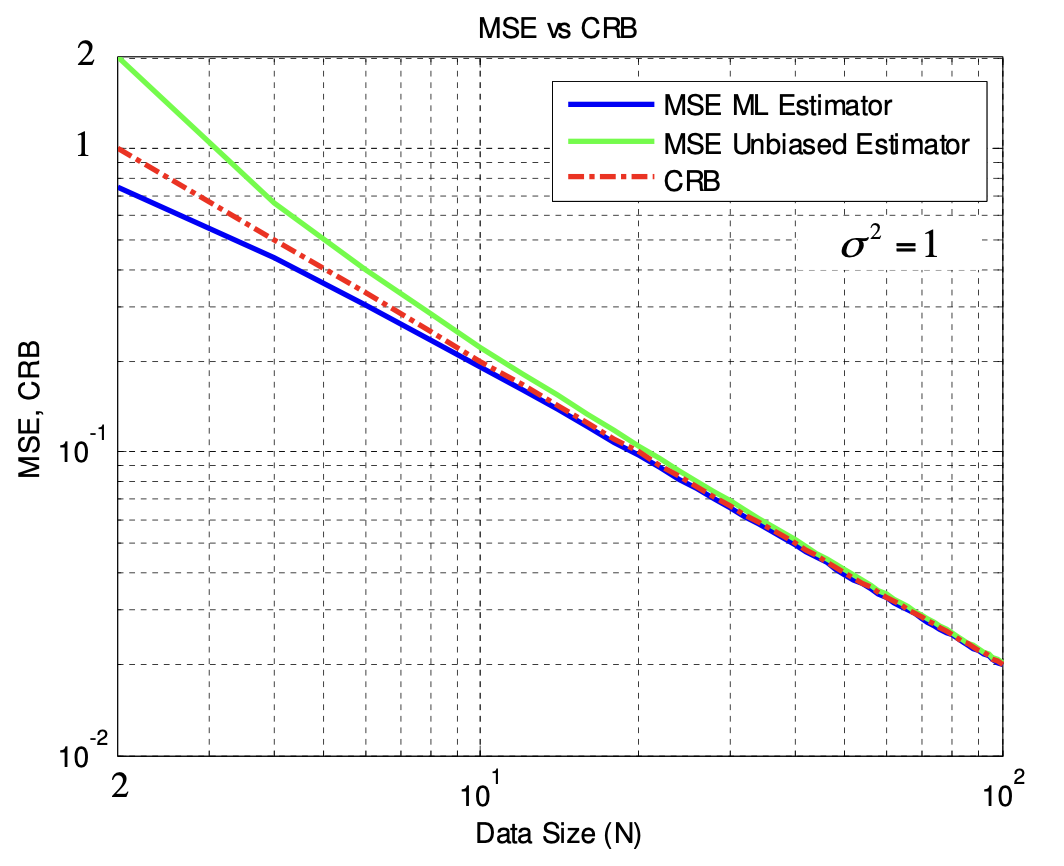
\includegraphics[width=0.55\linewidth]{Image/pdf 4/9.Graph 3.png}
    \label{fig:placeholder}
\end{figure}
\end{itemize}
\subsection{ML estimate of the Parameters of a Signal: Amplitude}
\begin{itemize}
    \item \textbf{Example}: We observe over the time interval \([0,T)\) a signal of known shape but unknown amplitude A, embedded in Additive White Gaussian Noise (AWGN):
    \begin{align*}
    X(t) &= A \cdot s(t) + W(t), \quad t \in [0, T] \\[1em]
    E_s &\triangleq \int_0^T s^2(t)\,dt < +\infty \\[1em]
    W(t) &\text{ AWGN:} \qquad S_W(f) = \frac{N_0}{2}
    \end{align*}
    \item Without loss of generality let us assume that \(X(t)\), \(s(t)\) and \(W(t)\) and A are real-valued.
    \item The first step is to transform the observed data in discrete format. To this purpose we have to choose the value of the essential bandwidth \(B\) at level \(\alpha\) of the useful signal \(s(t)\), in such a way that \(N=2BT\gg1\), so that \(\alpha\ll 1\).
    \item Once we have chosen \(B\), we can expand the signal in a base of \textit{sinc} functions:
    \[
    \mathbf{\Psi} \equiv \left\{ \psi_i(t) = \sqrt{2B} \cdot \operatorname{sinc}\left( 2B\left( t - \frac{i}{2B} \right) \right) \right\}_{i=0}^{2BT-1}
    \]
    \item i.e. we filter the continuous-time signal with a low pass filter of bandwidth \(B\) (\textit{anti-aliasing filter}) and we sample the filtered signal \(X_B(t)\) at intervals \(T_c=1/2B\):
\begin{figure}[H]
    \centering
    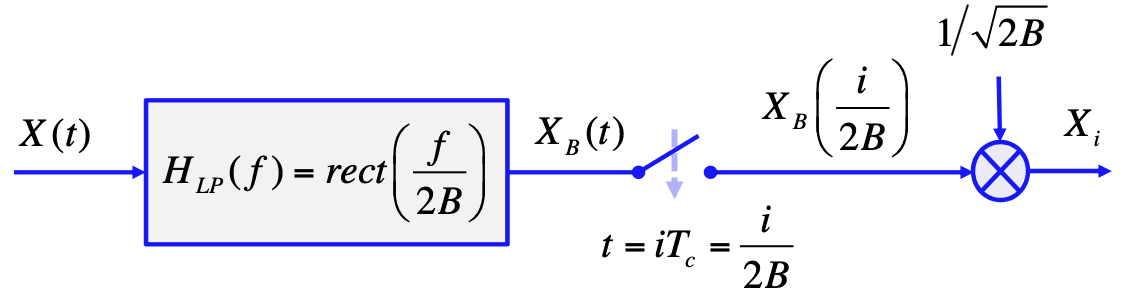
\includegraphics[width=0.6\linewidth]{Image/pdf 4/10.Anti-aliasing_filter.png}
    \label{fig:placeholder}
\end{figure}
    \item Since the bandwidth \(B\) has been selected so that \(2BT\gg 1\)and \(\alpha\ll1\), the useful signal passes undistorted the anti-aliasing filter \(s(t)\):
    \[
    X_B(t) = X(t) \otimes h_{LP}(t) = A \cdot s(t) \otimes h_{LP}(t) + W(t) \otimes h_{LP}(t) \approx A \cdot s(t) + W_B(t)
    \]
    \item In other words, the spectrum of the useful signal is not affected by the filter:
    \[
    S(f) H_{LP}(f) = S(f)\cdot \operatorname{rect}\left( \frac{f}{2B} \right) \approx S(f) \quad \text{if} \quad N = 2BT \gg 1
    \]
    \item Power Spectral Density (PSD) and power of the filtered (bandlimited) noise:
    \[
    S_{W_B}(f) = S_W(f) \left| H_{LP}(f) \right|^2 = \frac{N_0}{2} \, \operatorname{rect}\left( \frac{f}{2B} \right)
    \rightarrow
    \sigma_{W_B}^2 = \int_{-\infty}^{+\infty} S_{W_B}(f) \, df = N_0 B
    \]
    \begin{figure}[H]
        \centering
        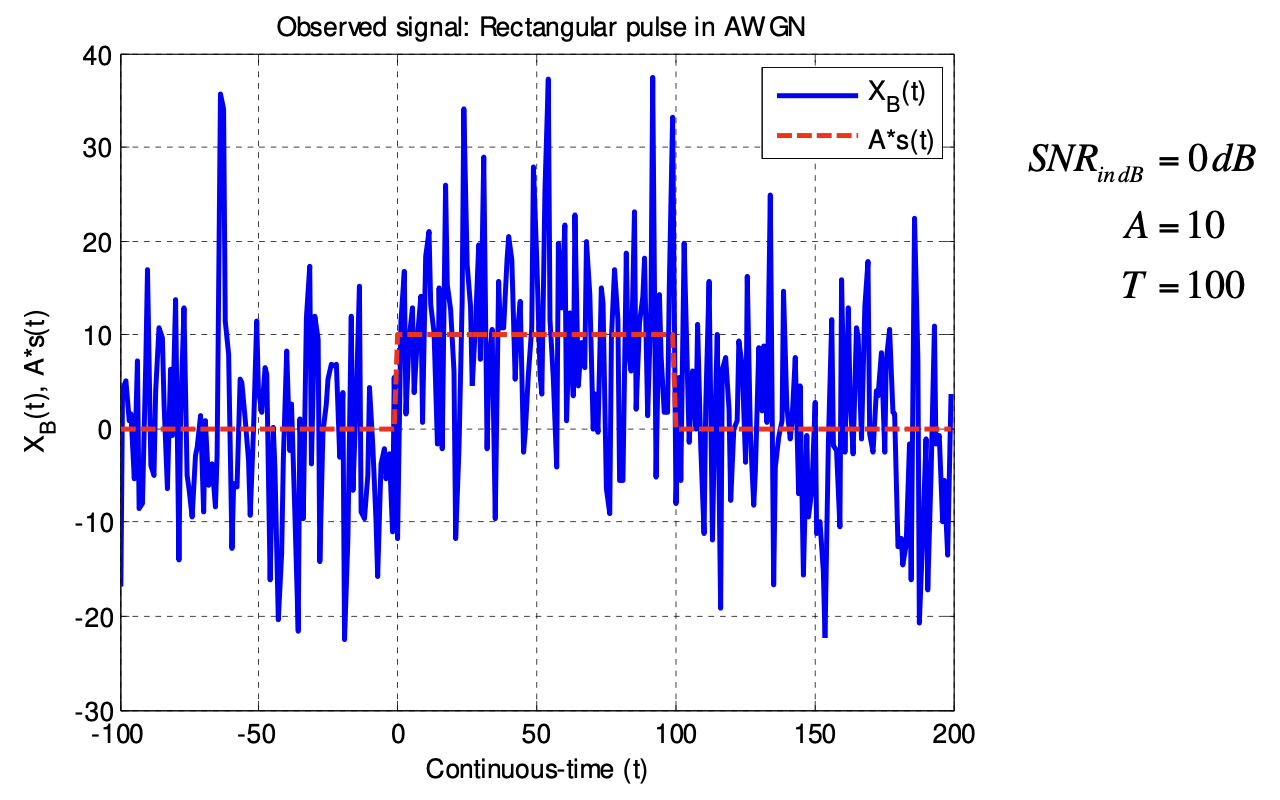
\includegraphics[width=0.6\linewidth]{Image/pdf 4/11.More_SNR.png}
        \label{fig:placeholder}
    \end{figure}
    \begin{figure}[H]
        \centering
        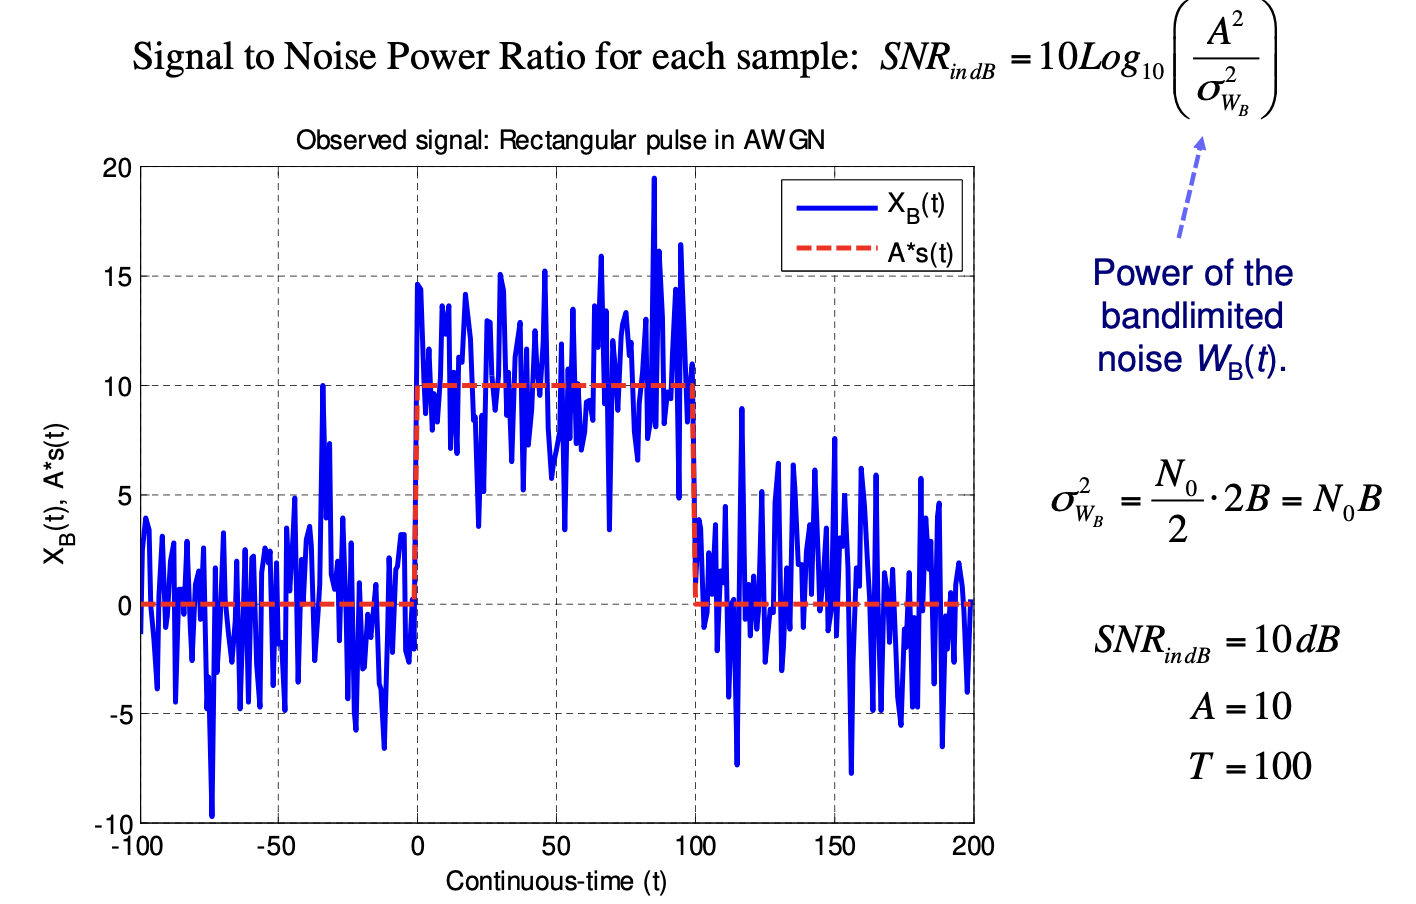
\includegraphics[width=0.6\linewidth]{Image/pdf 4/12.SNR_example.png}
        \label{fig:placeholder}
    \end{figure}
    \item The Autocorrelation Function (ACF) and the Power Spectral Density (PSD) of a process are related by the Fourier transform (\textbf{Wiener-Khintchine theorem}):
    \[
    R_{W_B}(\tau) \overset{\text{FT}}{\Longleftrightarrow} S_{W_B}(f)
    \]
    \[
    S_{W_B}(f) = \frac{N_0}{2} \operatorname{rect}\left( \frac{f}{2B} \right)
    \rightarrow
    R_{W_B}(\tau) \triangleq E \left\{ W_B(t) W_B(t+\tau) \right\} = N_0 B \cdot \operatorname{sinc}(2B\tau)
    \]
    \item The image of the observed (noisy) signal is:
    \[
    \mathbf{X} \triangleq \left[ 
    \frac{1}{\sqrt{2B}} X_B(0) \quad 
    \frac{1}{\sqrt{2B}} X_B\left( \frac{1}{2B} \right) \quad 
    \cdots \quad 
    \frac{1}{\sqrt{2B}} X_B\left( \frac{N-1}{2B} \right)
    \right]^T
    \]

    \[
    X_i \triangleq \frac{1}{\sqrt{2B}} X_B\left( \frac{i}{2B} \right) =
    \frac{A}{\sqrt{2B}} s\left( \frac{i}{2B} \right) +
    \frac{1}{\sqrt{2B}} W_B\left( \frac{i}{2B} \right)
    = A \cdot s_i + W_i, \qquad i = 0, 1, \cdots, N-1
    \]
    \[
    \mathbf{X} = A \cdot \mathbf{s} + \mathbf{W} \qquad \text{image of }\, X(t)\, \text{ for }\, t\in[0,T]
    \]
    \[
    s_i \triangleq \frac{1}{\sqrt{2B}} s\left(\frac{i}{2B}\right), \quad
    W_i \triangleq \frac{1}{\sqrt{2B}} W_B\left(\frac{i}{2B}\right), \quad
    i = 0, 1, \cdots, N-1
    \]
    \[
    \{ W_i \}_{i=0}^{N-1} \text{ are IID, and so } \{ X_i \}_{i=0}^{N-1} \text{ are mutually independent}
    \]

    \item The filterd noise is a Gaussian process, since it is obtained by filtering with a linear filter a Gaussian process. It is also zero mean, since the input noise is zero mean process:
    \[
    E\{W_i\} = E\left\{ \frac{1}{\sqrt{2B}} W_B \left( \frac{i}{2B} \right) \right\}
    = \frac{1}{\sqrt{2B}} E\left\{ W_B \left( \frac{i}{2B} \right) \right\}
    = \frac{1}{\sqrt{2B}} H_{LP}(0) \cdot E\{ W(t) \} = 0
    \]
    \item The samples of a Gaussian process are Gaussian random variables, so if they are \textbf{uncorrelated} they are also \textbf{independent}:
    \[
\begin{aligned}
\operatorname{cov}\{W_i, W_j\} &= E\{W_i W_j\} = E\left\{ \frac{1}{\sqrt{2B}} W_B\left(\frac{i}{2B}\right) \frac{1}{\sqrt{2B}} W_B\left(\frac{j}{2B}\right) \right\} \\
&= \frac{1}{2B} E\left\{ W_B\left(\frac{i}{2B}\right) W_B\left(\frac{j}{2B}\right) \right\}
= \frac{1}{2B} R_{W_B}\left( \frac{j-i}{2B} \right) \\
&= \frac{1}{2B} N_0 B \cdot \operatorname{sinc}\left( 2B \cdot \frac{j-i}{2B} \right)
= \frac{N_0}{2} \operatorname{sinc}(j - i) \\
&= 
\begin{cases}
\frac{N_0}{2}, & i = j \\
0, & i \neq j
\end{cases}
\end{aligned}
    \]
    \item Hence, the filterd noise samples \(\{W_i\}\) are zero-mean, Gaussian distributed, independent, with variance \(N_0/2\).
    \[
    \mathbf{X} = A \cdot \mathbf{s} + \mathbf{W} 
    \qquad \text{image of } X(t) \text{ for } t \in [0,T]
    \]

    \[
    s_i \triangleq \frac{1}{\sqrt{2B}} s\left( \frac{i}{2B} \right), \quad
    W_i \triangleq \frac{1}{\sqrt{2B}} W_B\left( \frac{i}{2B} \right), \quad i = 0,1,\cdots, N-1
    \]
    
    \[
    X_i \in \mathcal{N}(A \cdot s_i, \sigma^2_W), \qquad \left\{ X_i \right\}_{i=0}^{N-1} \text{ mutually independent}
    \]

    \[
    \sigma^2_W = \operatorname{var}\{W_i\} = \frac{1}{2B} \operatorname{var}\left\{ W_B\left( \frac{i}{2B} \right) \right\} = \frac{1}{2B} \left( 2B \cdot \frac{N_0}{2} \right) = \frac{N_0}{2}
    \]

    \[
    f_\mathbf{X} (\mathbf{x}; A) = \prod_{i=0}^{N-1} f_{X_i} (x_i; A)
    = \prod_{i=0}^{N-1} \frac{1}{\sqrt{\pi N_0}} \exp\left(-\frac{(x_i - A s_i)^2}{N_0}\right)
    = (\pi N_0)^{-N/2} \exp \left( -\frac{1}{N_0} \sum_{i=0}^{N-1} (x_i - A s_i)^2 \right )
    \]   
    \[
    \ln L(A) \triangleq \ln f_{\mathbf{X}}(\mathbf{x};A) 
    = \sum_{i=0}^{N-1} \ln f_{X_i}(x_i;A)
    = \kappa - \frac{1}{N_0} \sum_{i=0}^{N-1} (x_i - A s_i)^2
    \]
    \[
    \frac{d \ln L(A)}{dA}
    = \frac{2}{N_0} \sum_{i=0}^{N-1} s_i \left( x_i - A s_i \right)
    = \frac{2}{N_0} \left( \sum_{i=0}^{N-1} s_i x_i - A \sum_{i=0}^{N-1} s_i^2 \right)
    = \frac{2}{N_0} \left( \sum_{i=0}^{N-1} s_i x_i - A E_s \right)
    = \frac{2 E_s}{N_0} \left( \frac{1}{E_s} \sum_{i=0}^{N-1} s_i x_i -A \right)
    \]
    \[
    \text{where} \quad \sum_{i=0}^{N-1} s_i^2 = \| \mathbf{s} \|^2
    = (\mathbf{s}, \mathbf{s})
    = (s(t), s(t))
    = \int_0^T s^2(t) dt = E_s
    \]
    \[
    \hat{A}_{ML} = \frac{1}{E_s} \sum_{i=0}^{N-1} s_i x_i
    = \frac{1}{E_s} \mathbf{s}^T \mathbf{x}
    \]

    \[
    MSE\{\hat{A}_{ML}\} = CRB(A) = \frac{1}{I(A)} = \frac{N_0}{2E_s}
    \]
    \item The ML estimate of \(A\) is obtained by discrete-time FIR filtering the received data vector \textbf{x}.
    \item The FIR filter is called \textbf{Matched Filter (MF)} since its impulse response \textbf{h} is equal (i.e. matched) to the useful signal vector \textbf{s}, that is a propri known, since the signal shape is known.
\begin{figure}[H]
    \centering
    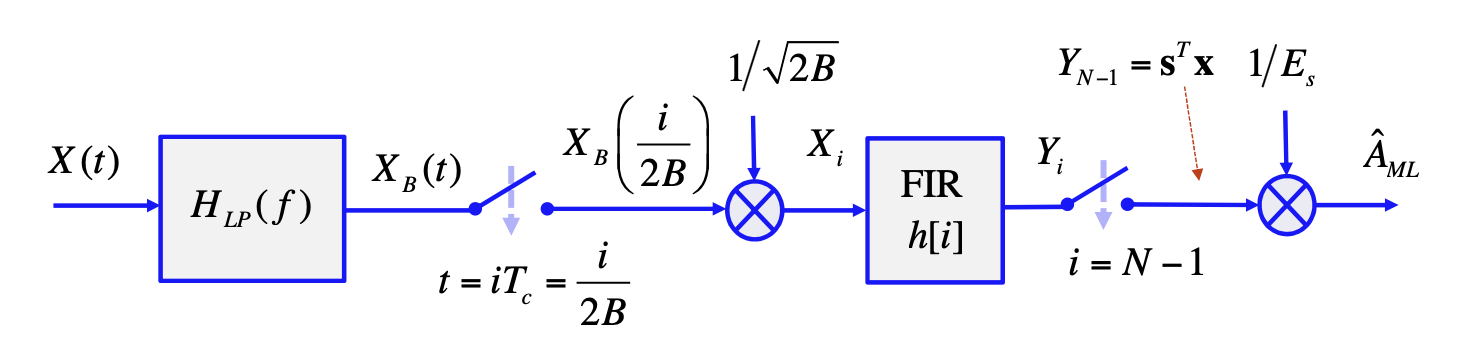
\includegraphics[width=0.75\linewidth]{Image/pdf 4/13.Matched_FIlter.png}
    \label{fig:placeholder}
\end{figure}
\[
\hat{A}_{ML} = \frac{1}{E_s} \sum_{i=0}^{N-1} s_i x_i = \frac{1}{E_s} \mathbf{s}^T \mathbf{x}
\]
    \textbf{Matched filter (MF)}: discrete-time FIR(N-1) filter with impulse response \(\textbf{h}=\textbf{s}\), i.e. to be precise:
    \[
    h[i]=[\textbf{h}]_{N-i}=s[N-1-i],\quad i=0,1,2,...,N-1
    \]
    \item The output of the MF is the cross-energy between the useful signal and the observed signal. It can be proved that if \(N\gg 1\), this cross-energy can be calculated by processing either the discrete-time data or the continuous-time data, we get the same result.
\[
    \begin{aligned}
&\sum_{i=0}^{N-1} s_i x_i = \mathbf{s}^T \mathbf{x} = (\mathbf{x}, \mathbf{s}) \quad\overset{\text{if } N \gg 1}{=} \quad (X(t), s(t)) = \int_0^T X(t) s(t) dt = E_{sx} 
\quad\text{cross-energy}\\[5pt]
&\hat{A}_{ML} = \frac{1}{E_s} \sum_{i=0}^{N-1} s_i x_i = \frac{1}{E_s} \mathbf{s}^T \mathbf{x} 
= \frac{E_{sx}}{E_s} = \frac{1}{E_s} \int_0^T X(t)s(t) dt \\
&= \frac{1}{\sqrt{E_s}} \int_0^T X(t) \frac{1}{\sqrt{E_s}} s(t) dt \\
&= \frac{1}{\sqrt{E_s}} \int_0^T X(t) \psi_1(t) dt 
= \frac{1}{\sqrt{E_s}} (X(t), \psi_1(t)) = \frac{1}{\sqrt{E_s}} X_1
\\[2em]
&\text{where } \psi_1(t) \triangleq \frac{1}{\sqrt{E_s}} s(t) \text{ has unit energy, i.e. unit norm}
\end{aligned}\]

    
    \item Analog implementation of the ML estimator through a \textbf{correlator}, i.e. a moving window integrator (MWI):
    \[
    X_1 \triangleq \int_{0}^{T} X(t)\psi_1(t)dt =
    \left[ \int_{t-T}^{t} X(\alpha)\psi_1(\alpha)d\alpha \right]_{t=T}
    \]
\begin{figure}[H]
    \centering
    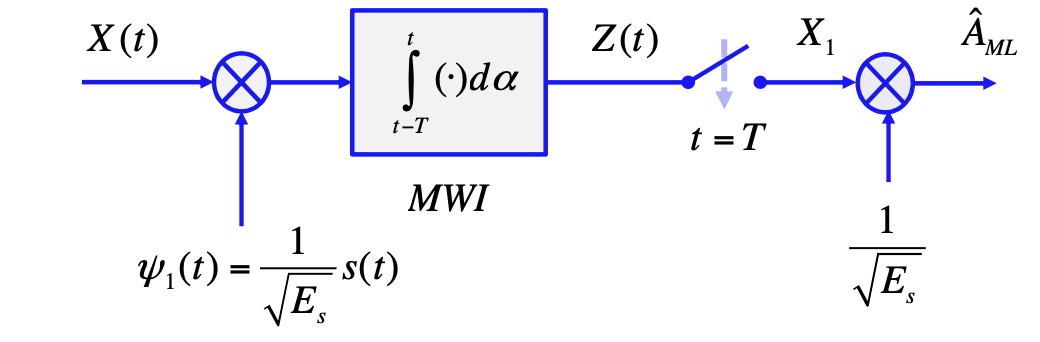
\includegraphics[width=0.75\linewidth]{Image/pdf 4/14.MWI.png}
    \label{fig:placeholder}
\end{figure}
\[
\text{Remind}: s(t)=rect\left(\frac{t-T/2}{T}\right)\quad\rightarrow\quad E_s=T
\]
    \item Analog implementation of the ML estimator through an analog \textbf{Matched Filter}:
    \[
    Z(t) = X(t) \otimes h(t) 
    = \int_0^T X(\alpha) h(t-\alpha) d\alpha 
    = \int_0^T X(\alpha) \psi_1(T-t+\alpha) d\alpha
    \]

    \[
    \text{where} \qquad h(t) \triangleq \psi_1(T-t) = \frac{1}{\sqrt{E_s}} s(T-t)
    \qquad\qquad
    \text{[ analog Matched Filter (MF) ]}
    \]

    \[
    X_1 \triangleq \int_0^T X(t)\psi_1(t)dt 
    = \int_0^T X(\alpha)\psi_1(\alpha) d\alpha 
    = \left[ X(t) \otimes \psi_1(T-t) \right]_{t=T}
    = Z(T)
    \]
    \begin{figure}[H]
        \centering
        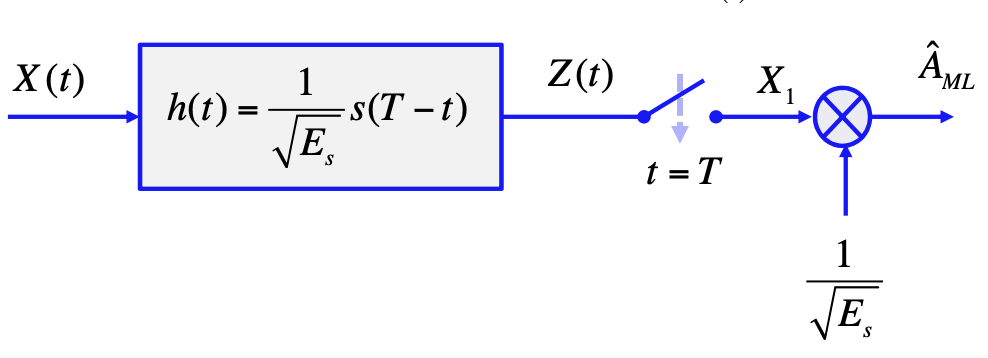
\includegraphics[width=0.6\linewidth]{Image/pdf 4/15.h(t).png}
        \label{fig:placeholder}
    \end{figure}
    \item The \textbf{Matched filter} can be implemented using digital or analog technology.
    \item We can implement a \textbf{matched filter} since we \textit{a-priori} known the signal shape (but not the amplitude).
    \item Matched filtering means calculate the inner product between the received vector \textbf{x} and the useful signal vector \(\textbf{s}\rightarrow\textbf{s}^T\textbf{x}\)(if the signal vector \textbf{s} is real).
    \item This tells us that \underline{matched filtering is equivalent to the orthogonal projection of the received data}\\
    \underline{vector \textbf{x} onto the 1D subspace generated by the signal vector \textbf{s}}.
    \item In other words, the only (principal) component we need to calculate is the one onto the direction of \textbf{s}. It is as if we calculate the \textbf{KLDT} where the first vector of the discrete-time basis is \textbf{s}(properly normalized) and we retain only the first component that is the one along \textbf{s}, the others being irrelevant.
    \[
\mathbf{x} = A \mathbf{s} + \mathbf{w} 
= A \sqrt{E_s} \cdot \frac{1}{\sqrt{E_s}} \mathbf{s} + \mathbf{w}
= A \sqrt{E_s} \mathbf{p} + \mathbf{w}
\]

\[
\text{where} \quad \mathbf{p} \triangleq \frac{1}{\sqrt{E_s}} \mathbf{s}
\quad\text{so that}\quad
\| \mathbf{p} \|^2 = \frac{\|\mathbf{s}\|^2}{E_s} = 1
\]

\[
\hat{A}_{ML} = \frac{1}{E_s} \mathbf{s}^T \mathbf{x}
= \frac{1}{\sqrt{E_s}} \mathbf{p}^T \mathbf{x}
= \frac{1}{\sqrt{E_s}} \left( A\sqrt{E_s}\mathbf{p}^T \mathbf{p} + \mathbf{p}^T \mathbf{w} \right)
= \frac{1}{\sqrt{E_s}} \left( A\sqrt{E_s} + \epsilon \sqrt{E_s} \right)
= A+\epsilon
\]

\[
\text{where} \quad \epsilon \triangleq \left( \mathbf{p}^T \mathbf{w} \right)/\sqrt{E_s}
\]
\begin{figure}[H]
    \centering
    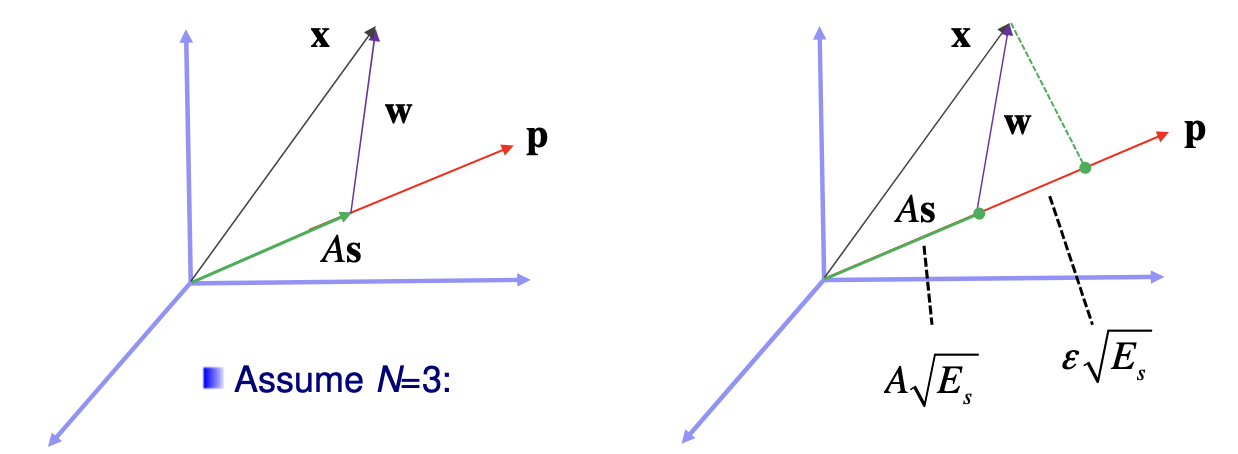
\includegraphics[width=0.75\linewidth]{Image/pdf 4/16.geometric_rep.png}
    \label{fig:placeholder}
\end{figure}
    \item \textbf{\underline{SNR at the output of the Matched Filter}}
    \item The ratio between the output and the input SNR is called \textbf{Processing Gain (PG)}.
    \item Let us calculate the input SNR (at the input of the digital Matched Filter i.e. after the anti-aliasing filter):
\[
\text{Signal to Noise Power Ratio at the input of the digital Matched Filter}
\]
\[
\text{SNR}_{\text{in}} = \frac{E \left\{ \|A\mathbf{s}\|^2 \right\}}{E \left\{ \|\mathbf{w}\|^2 \right\}}
= \frac{A^2 \|\mathbf{s}\|^2}{E \left\{ \sum_{i=1}^N W_i^2 \right\}}
= \frac{A^2 \|\mathbf{s}\|^2}{\sum_{i=1}^N E \left\{ W_i^2 \right\}}
= \frac{A^2 E_s}{N \cdot N_0 / 2}
\]
    \item The output of the Matche Filter (scaled by \(E_s\)) at discrete-time \(i=N-1\) provides the ML estimate of \(A\):
\[
\hat{A}_{ML} = \frac{1}{E_s}\mathbf{s}^T \mathbf{x}
= \frac{1}{E_s} \mathbf{s}^T (A \cdot \mathbf{s} + \mathbf{W})
= A \frac{1}{E_s} \mathbf{s}^T \mathbf{s} + \frac{1}{E_s} \mathbf{s}^T \mathbf{W}
= \underbrace{A}_{\text{useful signal component}}
+ \underbrace{\frac{1}{E_s} \mathbf{s}^T \mathbf{W}}_{\text{Estimation error}}
= A + \varepsilon
\]

\[
MSE = E\left\{ \varepsilon^2 \right\}
= E\left\{ \left( \frac{1}{E_s} \mathbf{s}^T \mathbf{W} \right)^2 \right\}
= \frac{1}{E_s^2} E\left\{ (\mathbf{s}^T \mathbf{W}) (\mathbf{s}^T \mathbf{W})^T \right\}
= \frac{1}{E_s^2} E\left\{ \mathbf{s}^T \mathbf{W} \mathbf{W}^T \mathbf{s} \right\}
\]

\[
= \frac{1}{E_s^2} \mathbf{s}^T E\left\{ \mathbf{W} \mathbf{W}^T \right\} \mathbf{s}
= \frac{1}{E_s^2} \mathbf{s}^T \mathbf{C}_W \mathbf{s}
= \frac{1}{E_s^2} \mathbf{s}^T \frac{N_0}{2} \mathbf{I} \mathbf{s}
= \frac{N_0}{2 E_s^2} \mathbf{s}^T \mathbf{s}
= \frac{N_0}{2 E_s}
\]

\[
\text{where} \quad \mathbf{C}_W \triangleq E\left\{ \mathbf{W} \mathbf{W}^T \right\}
= \frac{N_0}{2} \mathbf{I} ,
\quad \text{since } \operatorname{cov}\left\{ W_i, W_j \right\} =
\begin{cases}
\frac{N_0}{2} , & i = j \\
0, & i \neq j
\end{cases}
\]
    \item The signal to Noise power Ratio (SNR) at the output of the digital Matched Filter (scaled by \(E_s\)) at discrete-time \(i=N-1\) is given by:
    \[
SNR_{out} = \frac{A^2}{E\left\{ \varepsilon^2 \right\}}
= \frac{A^2}{N_0 / (2E_s)}
= \frac{A^2 E_s}{N_0/2}
\]

\[
SNR_{out} = \frac{A^2 E_s}{N_0/2}
= N \cdot \frac{A^2 E_s}{N \cdot N_0/2}
= N \cdot SNR_{in}
\]

\[
PG \triangleq \frac{SNR_{out}}{SNR_{in}} = N
\]
    \item \textbf{IMPORTANT}: The SNR at the output of the \textbf{Matched Filter} improves by a factor \(N\). Hence, the \textbf{processing gain} of the MF is given by the number \(N\) of processed samples.
    \item In the case of rectangular pulse, \(s(t)\) is constant over the observation interval so the amplitude \(A\) also represents the mean of the observed data:
    \[
s(t) = \mathrm{rect}\left( \frac{t - T/2}{T} \right)
\quad \Rightarrow \quad E_s = T
\]
\vspace{-1.5em}
\begin{align*}
\hat{A}_{ML} &= \frac{1}{E_s} \sum_{i=0}^{N-1} s_i x_i \\
&= \frac{1}{T} \sum_{i=0}^{N-1} \frac{1}{\sqrt{2B}} s\left(\frac{i}{2B}\right) \frac{1}{\sqrt{2B}} X\left(\frac{i}{2B}\right) \\
&= \frac{1}{2BT} \sum_{i=0}^{N-1} X\left( \frac{i}{2B} \right) \\
&= \frac{1}{N} \sum_{i=0}^{N-1} X \left( \frac{i}{2B} \right)
\qquad \leftarrow \text{Sample Mean of the observed data}
\end{align*}
\begin{figure}
    \centering
    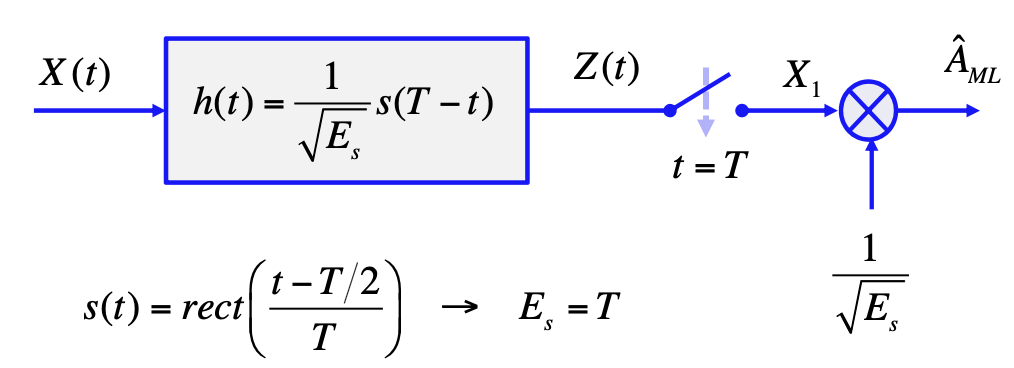
\includegraphics[width=0.75\linewidth]{Image/pdf 4/17.Remind_filt.png}
    \label{fig:placeholder}
\end{figure}
\[
Z(t) = X(t) \otimes h(t) = \left[ A \cdot s(t) + W_B(t) \right] \otimes h(t)
\]
\[
\phantom{Z(t)} = A \cdot s(t) \otimes h(t) + W_B(t) \otimes h(t)
\]
\[
\phantom{Z(t)} = Z_s(t) + Z_{W_B}(t)
\]

\[
\hat{A}_{ML} = \frac{1}{\sqrt{E_s}} X_1 = \frac{1}{\sqrt{T}} Z(T)
\]
\begin{figure}[H]
    \centering
    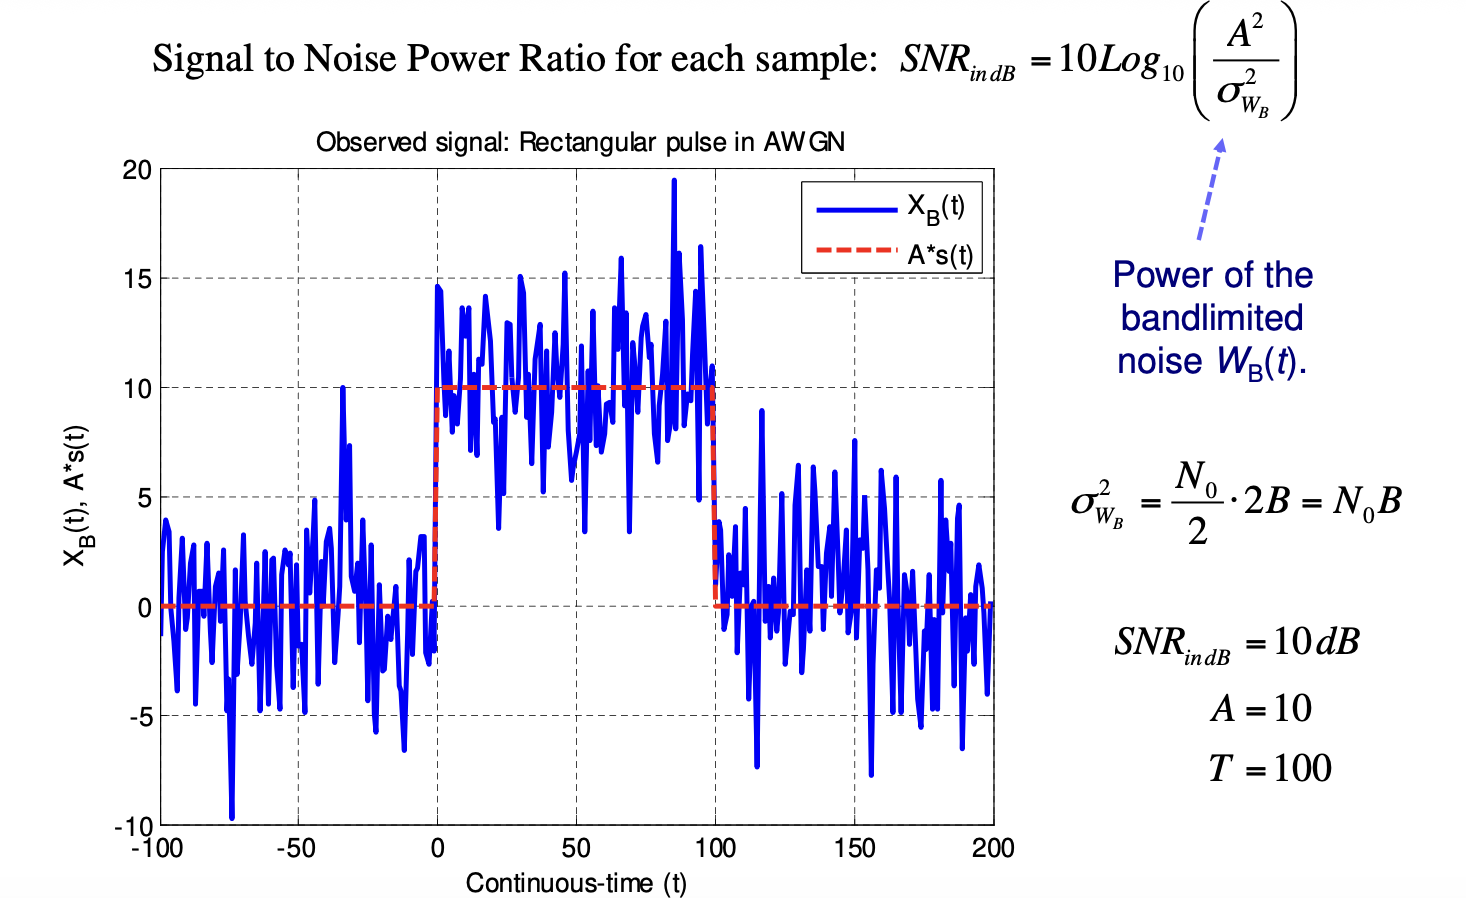
\includegraphics[width=0.75\linewidth]{Image/pdf 4/18.Example_Filter.png}
    \label{fig:placeholder}
\end{figure}
\begin{figure}[H]
    \centering
    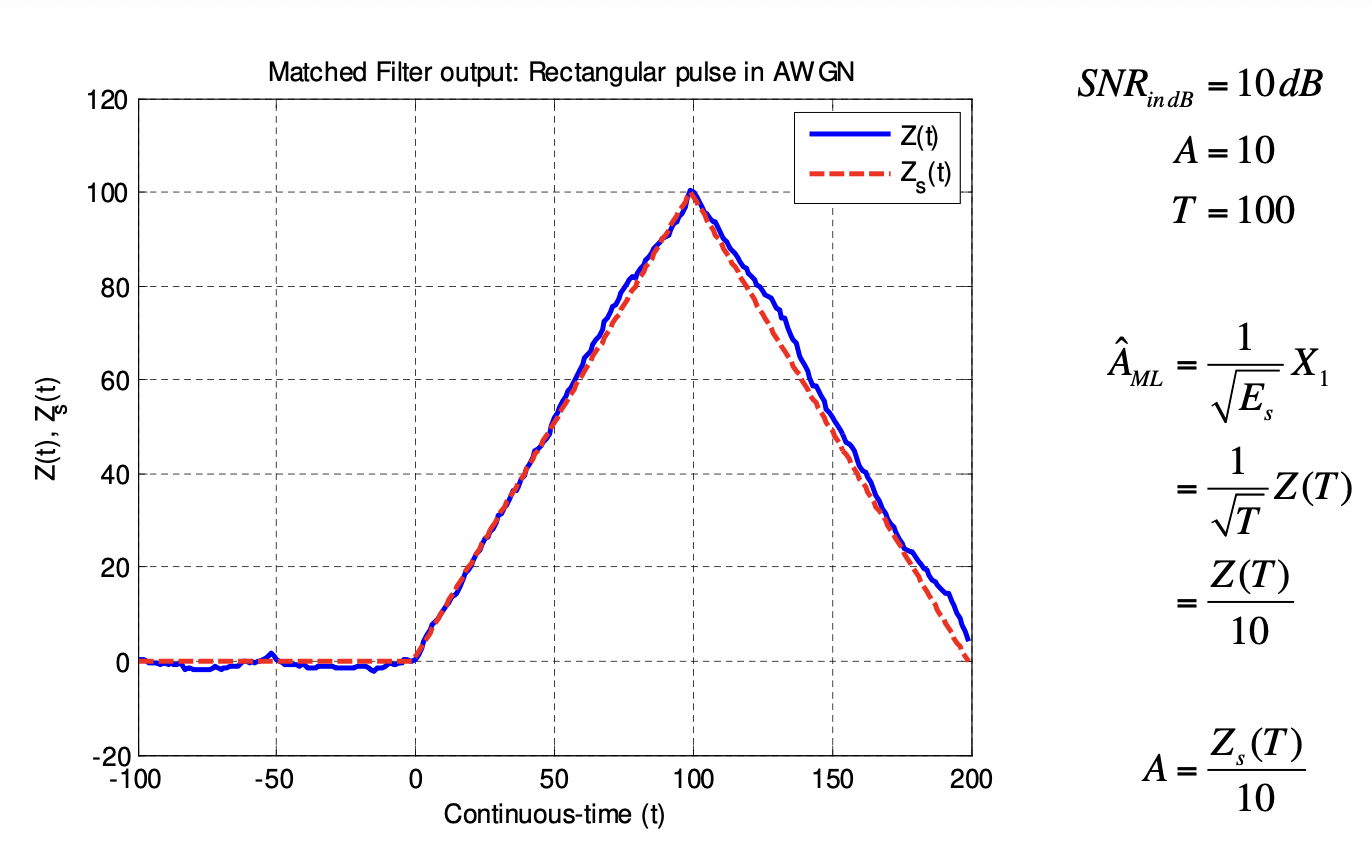
\includegraphics[width=0.70\linewidth]{Image/pdf 4/19.Output_matched.png}
    \label{fig:placeholder}
\end{figure}
\begin{figure}[H]
    \centering
    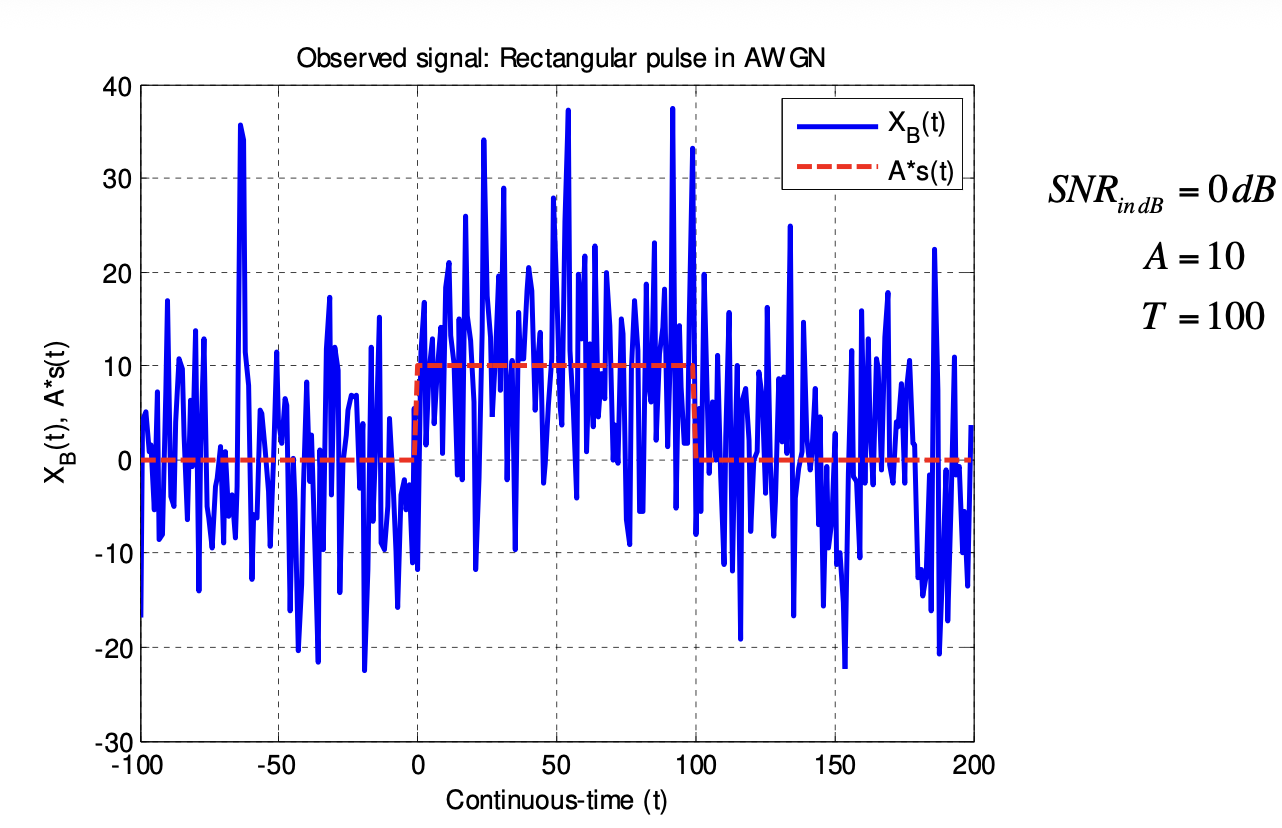
\includegraphics[width=0.70\linewidth]{Image/pdf 4/20.Other_example.png}
    \label{fig:placeholder}
\end{figure}
\begin{figure}
    \centering
    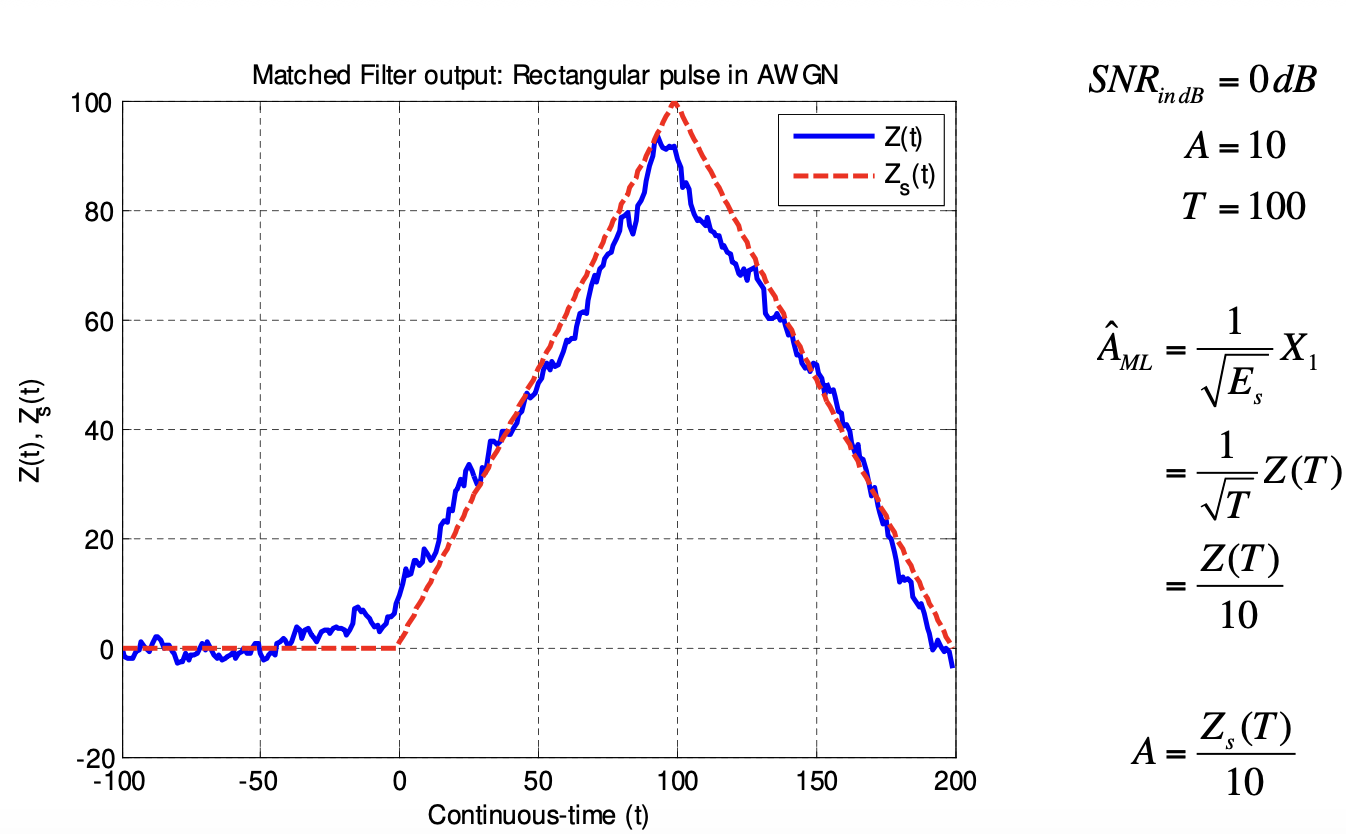
\includegraphics[width=0.70\linewidth]{Image/pdf 4/21.Matched_more_SNR.png}
    \label{fig:placeholder}
\end{figure}
    \item If the Time of Arrival (ToA) \(t_0\) is unknown, it should also be estimated
    The ToA can be estimted from the time the output of the MF (or the correlator) is maximum.
\begin{figure}[H]
    \centering
    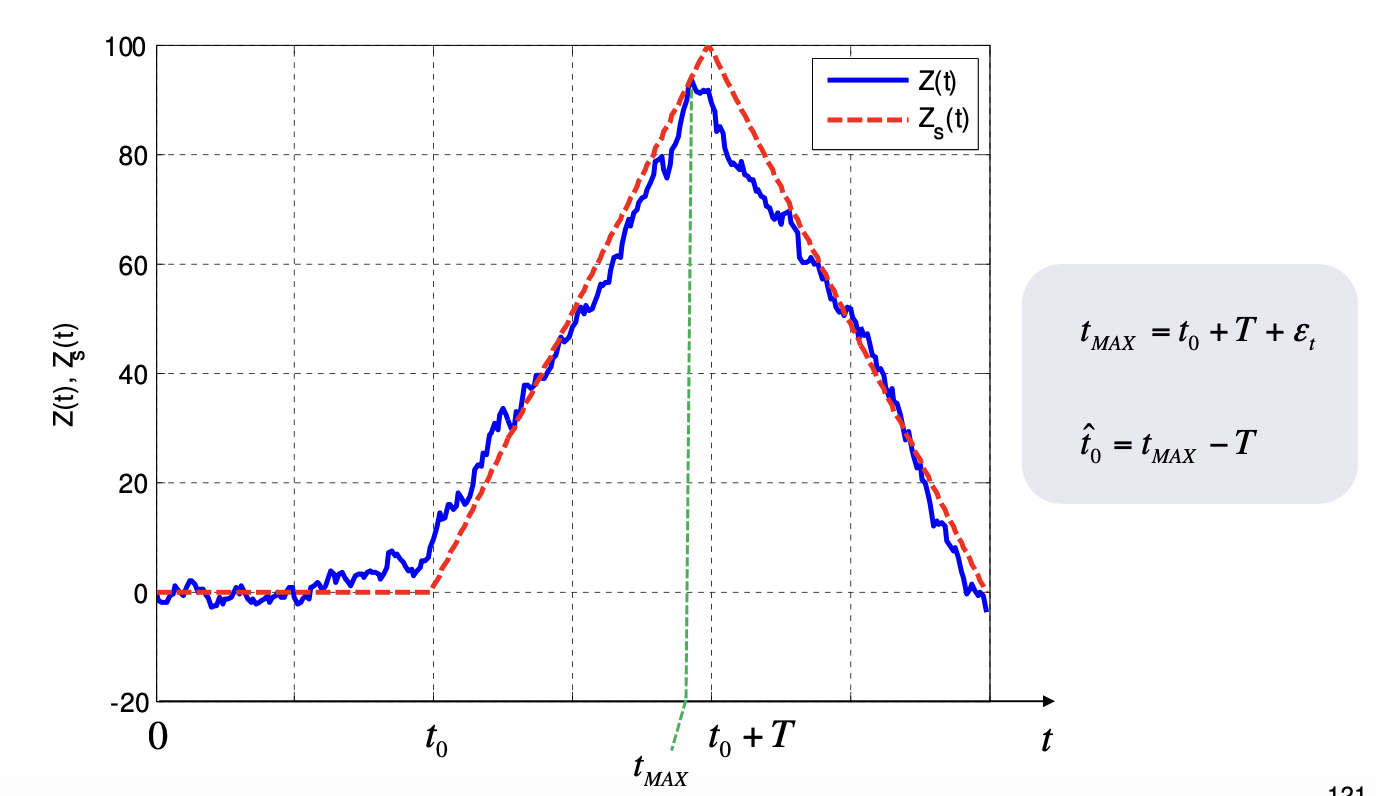
\includegraphics[width=0.7\linewidth]{Image/pdf 4/22.Estime_TOA.png}
    \label{fig:placeholder}
\end{figure}    
\end{itemize}

\subsection{ML Estimate of the Parameters of a Signal: Amplitude e Phase}
\begin{itemize}
    \item We observe a sinusoidal pulse \(s(t)\) with constant envelope over the time interval \([0,T)\). The carrier frequency \(f_0\) is perfectly known and \underline{we want to estimate the unknown signal amplitude \(A\) and phase \(\theta\)}. The signal is received corrupted by Additive White Gaussian Noise (AWGN):
    \[
    X(t) = s(t) + W(t) = A \cdot p(t) + W(t), \quad t \in [0, T]
    \]
    \[
    E_s \triangleq \int_{0}^{T} A^2 p^2(t) dt = A^2 E_p = \frac{A^2 T}{2} < +\infty
    \]
    \[
    W(t) \text{~AWGN:} \quad S_w(f) = \frac{N_0}{2}
    \]
    \[
    p(t) = \cos(2\pi f_0 t + \theta)~\mathrm{rect}\left( \frac{t - T/2}{T} \right),
    \quad \text{with } f_0~\text{known}, \quad f_0 T \gg 1
    \]
    \item The energy of the signal \(p(t)\) is:
    \[
E_p = \int_{0}^{T} p^2(t) dt
= \int_{0}^{T} \cos^2(2\pi f_0 t + \theta) dt
= \int_{0}^{T} \left[ \frac{1}{2} + \frac{1}{2}\cos(4\pi f_0 t + 2\theta) \right] dt
\]

\[
= \frac{1}{2} \int_0^T dt + \frac{1}{2} \int_0^T \cos(4\pi f_0 t + 2\theta) dt
= \frac{T}{2} \left( 1 + \frac{1}{T} \int_0^T \cos(4\pi f_0 t + 2\theta) dt \right)
\]

\[
\cong \frac{T}{2}
\]

\[
\text{In fact:} \quad \frac{1}{T} \int_0^T \cos(4\pi f_0 t + 2\theta) dt \ll 1 \quad \text{if} \quad f_0 T \gg 1
\]
    \item The spectrum of the signal \(p(t)\) is given by its the Fourier Transform (FT):
    \[
P(f) = FT\left\{ p(t) \right\} 
= \frac{T}{2} \, \mathrm{sinc} \big( (f + f_0)T \big)
e^{-j\theta} e^{-j\pi(f + f_0)T}
+ \frac{T}{2} \, \mathrm{sinc} \big( (f - f_0)T \big)
e^{j\theta} e^{-j\pi(f - f_0)T}
\]
\begin{figure}[H]
    \centering
    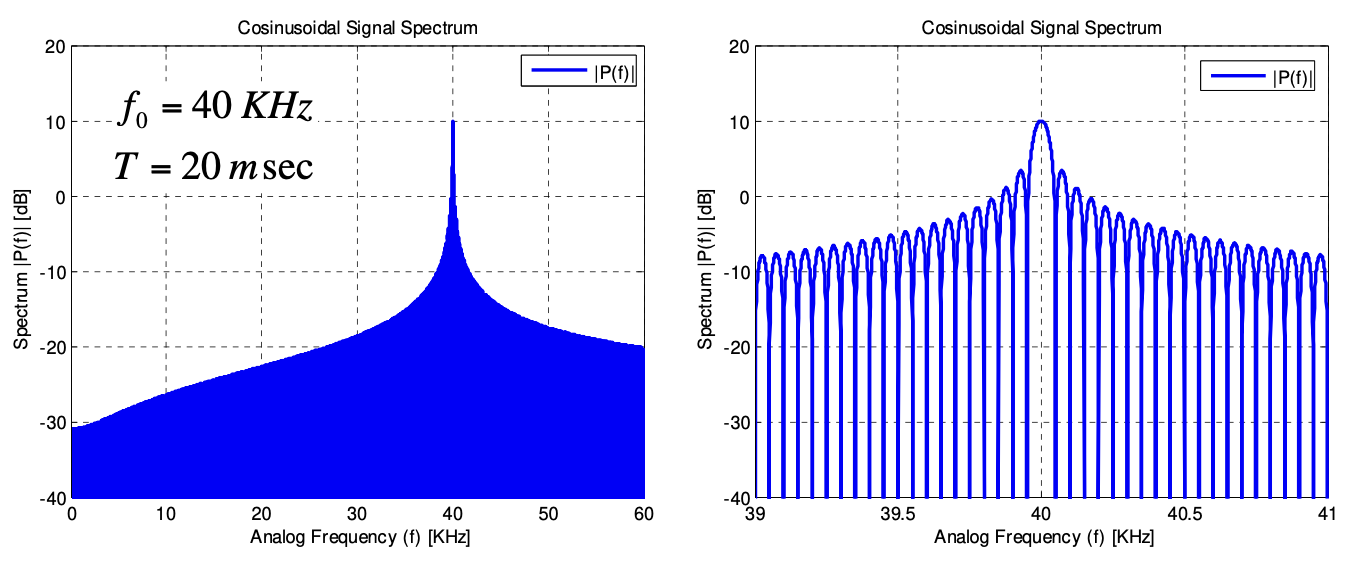
\includegraphics[width=0.75\linewidth]{Image/pdf 4/23.Cos_spectrum.png}
    \label{fig:placeholder}
\end{figure}
    \item The FT of the useful signal \(s(t)=Ap(t)\) calculated at the known central frequency \(f_0\):
    \[
    A \cdot P(f_0) = \frac{A T}{2} \, \mathrm{sinc}(2 f_0 T) \, e^{-j\theta} e^{-j 2\pi f_0 T}
    + \frac{A T}{2} \, e^{j\theta}
    \cong \frac{A T}{2} e^{j\theta}
    \quad \text{if} \quad f_0 T \gg 1
    \]
    \item Note that the amplitude and phase of \(A\cdot P(f_0)\) contains the information on the unknown parameters \(A\) and \(\theta\).
    \item The FT of the signal of interest \(s(t)=Ap(t)\) calculated at the known frequency \(f_0\):
\[
S(f_0) = FT\left\{ s(t) \right\}\Big|_{f=f_0}
= A \cdot P(f_0)
\cong \frac{A T}{2} e^{j\theta}
\quad \text{if} \quad f_0 T \gg 1
\]

    \item Hence, the amplitude and phase of \(A\cdot P(f_0)\) contains the information on the unknown parameters \(A\) and \(\theta\).
    \item \underline{In the absence of noise}, we can retrieve the true value of the amplitude and the phase from the FT of received signal \(X(t)=s(t)\) as follows:
    \[
X(f_0) = S(f_0) = FT\left\{ s(t) \right\}\Big|_{f=f_0} = A \cdot P(f_0) \cong \frac{AT}{2} e^{j\theta} \quad \text{if} \quad f_0 T \gg 1
\]

\[
\Rightarrow
\begin{cases}
A = \frac{2}{T} |S(f_0)| = \frac{2}{T} |X(f_0)| \\[10pt]
\theta = \angle S(f_0) = \angle X(f_0)
\end{cases}
\qquad 
\text{where } X(f_0) = FT\{ X(t) \}\Big|_{f=f_0}
\]
    \item \underline{When the noise is present}, the FT of the received signal \(X(t)\) represents an estimate of the FT of the signal of interest \(s(t)\). Hence, we can use the previous relationships to estimate the amplitude and the phase of \(s(t)\) from the FT of received (noisy) signal \(X(t)\):
    \[
    \left\{
    \begin{aligned}
    \hat{A}_{MM} &= \frac{2}{T} |\hat{S}(f_0)| = \frac{2}{T} |X(f_0)| \\
    \hat{\theta}_{MM} &= \angle \hat{S}(f_0) = \angle X(f_0)
    \end{aligned}
    \right.
    \qquad
    \text{where} \quad X(f_0) = FT \left\{ X(t) \right\} \Big|_{f = f_0}
    \]

    \item The estimators derived in this way are a sort of \textbf{Method of Moment estimators}, since the estimate is obtained by exploiting the relationship between the unknown parameters and a "moment" of the data, i.e. the data Fourier Transform at the frequency \(f_0\)(which is the frequency where the signal spectrum is maximum).
    \item As in the previous case, the received signal is converted in discrete form by \textit{anti-aliasing} filtering and sampling the filtered signal \(X_B(t)\) at intervals \(T_c=1/2B\), where \(B\gg f_0\).
\begin{figure}[H]
    \centering
    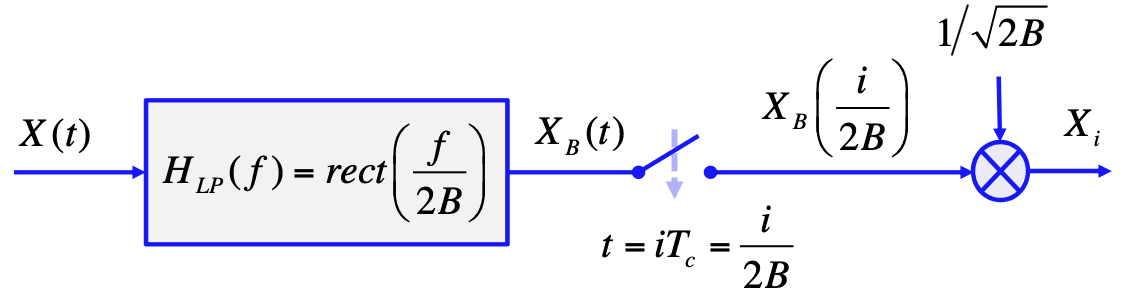
\includegraphics[width=0.75\linewidth]{Image/pdf 4/10.Anti-aliasing_filter.png}
    \label{fig:placeholder}
\end{figure}
\[
X_i \triangleq \frac{1}{\sqrt{2B}} X_B\left(\frac{i}{2B}\right)
= \frac{A}{\sqrt{2B}} p\left(\frac{i}{2B}\right)
+ \frac{1}{\sqrt{2B}} W_B\left(\frac{i}{2B}\right)
= A \cdot p_i(\theta) + W_i, \qquad i = 0, \ldots, N-1
\]

\[
p_i(\theta) \triangleq \frac{1}{\sqrt{2B}} p\left(\frac{i}{2B}\right)
= \frac{1}{\sqrt{2B}} \cos\left(2\pi f_0 \frac{i}{2B} + \theta\right), \qquad
W_i \triangleq \frac{1}{\sqrt{2B}} W_B\left(\frac{i}{2B}\right)
\]

\[
X_i \in \mathcal{N}\left(A \cdot p_i(\theta), \sigma_W^2\right), \qquad
\left\{X_i\right\}_{i=0}^{N-1} \text{ are mutually independent}
\]
\vspace{0.5em}
\[
\mathbf{X} \text{ image of } X(t) \text{ for } t \in [0, T]
\]
\[
\mathbf{X} =
\begin{bmatrix}
X_0 \\ X_1 \\ \vdots \\ X_{N-1}
\end{bmatrix}
= A \cdot \mathbf{p}(\theta) + \mathbf{W}
=
\begin{bmatrix}
\frac{A}{\sqrt{2B}} \cos(\theta) \\
\frac{A}{\sqrt{2B}} \cos\left(2\pi f_0 \frac{1}{2B} + \theta \right) \\
\vdots \\
\frac{A}{\sqrt{2B}} \cos\left(2\pi f_0 \frac{N-1}{2B} + \theta \right)
\end{bmatrix}
+ 
\begin{bmatrix}
W_0 \\ W_1 \\ \vdots \\ W_{N-1}
\end{bmatrix}
\]

\[
W_i \in \mathcal{N}(0, \sigma^2_W),\quad \text{where } \sigma^2_W = \mathrm{var}\{W_i\} = \frac{N_0}{2} \quad \Longrightarrow \quad X_i \in \mathcal{N}(A \cdot p_i(\theta), \sigma^2_W)
\]

\[
p_i(\theta) = \frac{1}{\sqrt{2B}} \cos\left(2\pi f_0 \frac{i}{2B} + \theta\right) 
= \frac{1}{\sqrt{2B}} \cos(2\pi F_0 i + \theta)
\]

\[
F_0 \triangleq \frac{f_0}{2B} \qquad \text{Digital Frequency - Nyquist Sampling} \qquad 0 < F_0 < \frac{1}{2}
\]
    \item The input Signal to Noise power Ratio (\(SNR_{in}\)):
\[
SNR_{in} = \frac{\left\|\mathbf{A} \cdot \mathbf{p}(\theta)\right\|^2}{E\left\{\|\mathbf{W}\|^2\right\}}
= \frac{A^2 \|\mathbf{p}(\theta)\|^2}{E\left\{ \|\mathbf{W}\|^2 \right\}}
= \frac{A^2}{2B} \cdot \frac{N}{2} \cdot \frac{2}{N_0N}
= \frac{A^2}{2N_0B}
\]

\[
\|\mathbf{p}(\theta)\|^2 = \sum_{i=0}^{N-1} \left[ p_i(\theta) \right]^2
= \frac{N}{2B} \cdot \frac{1}{N} \sum_{i=0}^{N-1} \cos^2(2\pi F_0 i + \theta)
\approx \frac{N}{2B} \cdot \frac{1}{2}
\]

\[
E\left\{ \|\mathbf{W}\|^2 \right\}
= E\left\{ \sum_{i=0}^{N-1} W_i^2 \right\}
= \sum_{i=0}^{N-1} E\left\{ W_i^2 \right\}
= N \sigma_W^2 = N \cdot \frac{N_0}{2}
\]

    \item Joint pdf of the observed data:
\[
f_{\mathbf{X}}(\mathbf{x};A,\theta)
= \prod_{i=0}^{N-1} f_{X_i}(x_i;A,\theta)
= \prod_{i=0}^{N-1} \frac{1}{\sqrt{\pi N_0}}
\exp\left[-\frac{1}{N_0} \left(x_i - \frac{A}{\sqrt{2B}} \cos(2\pi F_0 i + \theta)\right)^2 \right]
\]
\[
= (\pi N_0)^{-N/2}
\exp\left[-\frac{1}{N_0} \sum_{i=0}^{N-1} \left(x_i - \frac{A}{\sqrt{2B}} \cos(2\pi F_0 i + \theta)\right)^2 \right]
\]
    \item The log-likelihood function (log-LF):
    \[
\ln L(A, \theta)
= \ln f_{\mathbf{X}}(\mathbf{x};A,\theta)
= -\frac{N}{2} \ln(\pi N_0)
- \frac{1}{N_0} \sum_{i=0}^{N-1}
\left( x_i - \frac{A}{\sqrt{2B}} \cos(2\pi F_0 i + \theta) \right)^2
\]
\[
= -\frac{N}{2} \ln(\pi N_0)
- \frac{1}{N_0} \sum_{i=0}^{N-1} x_i^2
- \frac{A^2}{N_0 2B} \sum_{i=0}^{N-1} \cos^2(2\pi F_0 i + \theta)
+ \frac{2A}{N_0 \sqrt{2B}} \sum_{i=0}^{N-1} x_i \cos(2\pi F_0 i + \theta)
\]
\[
\cong \kappa
- \frac{A^2}{N_0 2B} \cdot \frac{N}{2}
+ \frac{2A}{N_0 \sqrt{2B}} \sum_{i=0}^{N-1} x_i \cos(2\pi F_0 i + \theta)
\]
\vspace{0.5em}
\[
\text{In fact, if } N \gg 1:
\]
\[
\frac{1}{N} \sum_{i=0}^{N-1} \cos^2 (2\pi F_0 i + \theta)
= \frac{1}{N} \sum_{i=0}^{N-1} \left[ \frac{1}{2} + \frac{1}{2} \cos(4\pi F_0 i + 2\theta) \right]
= \frac{1}{2} \left( 1 + \frac{1}{N} \sum_{i=0}^{N-1} \cos(4\pi F_0 i + 2\theta) \right)
\cong \frac{1}{2}
\]
\[
\frac{1}{N} \sum_{i=0}^{N-1} \sin^2 (2\pi F_0 i + \theta) \cong \frac{1}{2}
\]
\[
\frac{1}{N} \sum_{i=0}^{N-1} \cos(2\pi F_0 i + \theta) \sin(2\pi F_0 i + \theta)
= \frac{1}{2N} \sum_{i=0}^{N-1} \sin(4\pi F_0 i + 2\theta) \cong 0
\]

    \item The \textbf{joint ML estimators} of \(A\) and \(\theta\) are obtained by jointly solving the two \textbf{likelihood equations}, which are obtained by deriving the log-LF with respect to both the unknown parameters:
    \[
\left\{
\begin{aligned}
&\frac{\partial \ln L(A,\theta)}{\partial A} = 0 \\
&\frac{\partial \ln L(A,\theta)}{\partial \theta} = 0
\end{aligned}
\right.
\]
\[
\frac{\partial \ln L(A,\theta)}{\partial A}
= \frac{\partial}{\partial A} \left[
-\frac{A^2}{N_0 2B} \cdot \frac{N}{2}
+ \frac{2A}{N_0 \sqrt{2B}} \sum_{i=0}^{N-1} x_i \cos(2\pi F_0 i + \theta)
\right]
\]
\[
= -\frac{AN}{N_0 2B}
+ \frac{2}{N_0 \sqrt{2B}}
\sum_{i=0}^{N-1} x_i \cos(2\pi F_0 i + \theta)
= 0
\]
\[
\implies
A = \sqrt{2B} \cdot \frac{2}{N} \sum_{i=0}^{N-1} x_i \cos(2\pi F_0 i + \theta)
\]
\[
\frac{\partial \ln L(A,\theta)}{\partial \theta}
= \frac{\partial}{\partial \theta}
\left[
    -\frac{A^2}{N_0 2B} \cdot \frac{N}{2}
    + \frac{2A}{N_0 \sqrt{2B}}
    \sum_{i=0}^{N-1}
    x_i \cos(2\pi F_0 i + \theta)
\right]
= -\frac{2A}{N_0 \sqrt{2B}}
\sum_{i=0}^{N-1} x_i \sin(2\pi F_0 i + \theta)
= 0
\]

\[
\sum_{i=0}^{N-1}
x_i \sin(2\pi F_0 i + \theta)
=
\sum_{i=0}^{N-1}
x_i \left[
    \sin(2\pi F_0 i) \cos(\theta)
    + \cos(2\pi F_0 i) \sin(\theta)
\right]
= 0
\]

\[
\sum_{i=0}^{N-1}
x_i \cos(2\pi F_0 i) \sin(\theta)
= -\sum_{i=0}^{N-1}
x_i \sin(2\pi F_0 i) \cos(\theta)
\]

\[
\frac{\sin(\theta)}{\cos(\theta)}
=
-\frac{ \sum_{i=0}^{N-1} x_i \sin(2\pi F_0 i) }
        { \sum_{i=0}^{N-1} x_i \cos(2\pi F_0 i) }
\implies
\theta = -\arctan
\left(
\frac{ \sum_{i=0}^{N-1} x_i \sin(2\pi F_0 i) }
      { \sum_{i=0}^{N-1} x_i \cos(2\pi F_0 i) }
\right)
\]
    \item Hence, the ML estimator of \(\theta\) is given by:
    \[
\hat{\theta}_{ML}
= -\arctan \left(
    \frac{\sum_{i=0}^{N-1} x_i \sin(2\pi F_0 i)}
         {\sum_{i=0}^{N-1} x_i \cos(2\pi F_0 i)}
\right)
= -\arctan \left(
    \frac{ \mathbf{s}^T \mathbf{x} }
         { \mathbf{c}^T \mathbf{x} }
\right)
\]

\[
\text{where we defined the two orthonormal (orthogonal and unit norm) vectors:}
\]
\[
\mathbf{c} \triangleq [c_0, c_1, \ldots, c_{N-1}],
\quad
c_i \triangleq \sqrt{\frac{2}{N}} \cos(2\pi F_0 i),
\quad \|\mathbf{c}\|^2 = \mathbf{c}^T \mathbf{c} = 1
\]
\[
\mathbf{s} \triangleq [s_0, s_1, \ldots, s_{N-1}],
\quad
s_i \triangleq \sqrt{\frac{2}{N}} \sin(2\pi F_0 i),
\quad \|\mathbf{s}\|^2 = \mathbf{s}^T \mathbf{s} = 1
\]
\[
\mathbf{s}^T\mathbf{c} = \mathbf{c}^T\mathbf{s} = 0
\implies \mathbf{s} \perp \mathbf{c}
\]
    \item Now, we should insert the ML estimate of \(\theta\) in the previous expression of \(A\):
\begin{align*}
\hat{A}_{ML} &= \sqrt{2B} \cdot \frac{2}{N} \sum_{i=0}^{N-1} x_i \cos \left(2\pi F_0 i + \hat{\theta}_{ML}\right)\\
&= \sqrt{2B} \cdot \frac{2}{N} \sum_{i=0}^{N-1} x_i \cos(2\pi F_0 i) \cos(\hat{\theta}_{ML})
- \sqrt{2B} \cdot \frac{2}{N} \sum_{i=0}^{N-1} x_i \sin(2\pi F_0 i) \sin(\hat{\theta}_{ML})\\
&= \sqrt{2B} \sqrt{ \frac{2}{N} } \left( \mathbf{c}^T \mathbf{x} \cos(\hat{\theta}_{ML}) - \mathbf{s}^T \mathbf{x} \sin(\hat{\theta}_{ML}) \right)\\
&\overset{N=2BT}{=} \sqrt{\frac{2}{T}} \left( (\mathbf{c}^T \mathbf{x}) \cos(\hat{\theta}_{ML}) - (\mathbf{s}^T \mathbf{x}) \sin(\hat{\theta}_{ML}) \right)
\end{align*}
    \begin{figure}[H]
        \centering
        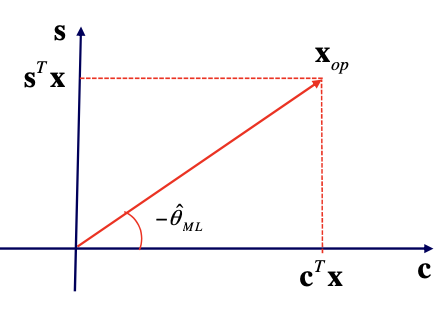
\includegraphics[width=0.75\linewidth]{Image/pdf 4/24.Rapp_geom.png}
        \label{fig:placeholder}
    \end{figure}   
    \item Where \(\mathbf{x}_{op}\) is the orthogonal projection of the received \(N\)-dim vector \textbf{x} onto the plane generated by the orthonormal vectors \textbf{c} and \textbf{s}(which is the \textbf{signal subspace}):
\[
\left\{
\begin{aligned}
&\cos(\hat{\theta}_{ML}) = \cos(-\hat{\theta}_{ML}) = \frac{\mathbf{c}^T \mathbf{x}}{\sqrt{(\mathbf{c}^T\mathbf{x})^2 + (\mathbf{s}^T\mathbf{x})^2}} \\
&-\sin(\hat{\theta}_{ML}) = \sin(-\hat{\theta}_{ML}) = \frac{\mathbf{s}^T \mathbf{x}}{\sqrt{(\mathbf{c}^T\mathbf{x})^2 + (\mathbf{s}^T\mathbf{x})^2}}
\end{aligned}
\right.
\]

\[
\text{with} \quad \mathbf{c}^T\mathbf{x} = \mathbf{c}_{op}^T\mathbf{x}, \qquad
\mathbf{s}^T\mathbf{x} = \mathbf{s}_{op}^T\mathbf{x}
\]
    \item The ML estimator of \(A\) is immediately derived:
    \[
\begin{aligned}
\hat{A}_{ML} &= \sqrt{\frac{2}{T}}
    \left[
        (\mathbf{c}^T\mathbf{x})\cos(\hat{\theta}_{ML})
        - (\mathbf{s}^T\mathbf{x})\sin(\hat{\theta}_{ML})
    \right]\\
&= \sqrt{\frac{2}{T}}
    \left[
        (\mathbf{c}^T\mathbf{x})\cos(\hat{\theta}_{ML})
        + (\mathbf{s}^T\mathbf{x})\sin(-\hat{\theta}_{ML})
    \right]\\
&= \sqrt{\frac{2}{T}}
    \left[
        (\mathbf{c}^T\mathbf{x}) \frac{\mathbf{c}^T\mathbf{x}}{ \sqrt{ (\mathbf{c}^T\mathbf{x})^2 + (\mathbf{s}^T\mathbf{x})^2 } }
        + (\mathbf{s}^T\mathbf{x}) \frac{\mathbf{s}^T\mathbf{x}}{ \sqrt{ (\mathbf{c}^T\mathbf{x})^2 + (\mathbf{s}^T\mathbf{x})^2 } }
    \right]\\
&= \sqrt{\frac{2}{T}}
    \left[
        \frac{(\mathbf{c}^T\mathbf{x})^2}{ (\mathbf{c}^T\mathbf{x})^2 + (\mathbf{s}^T\mathbf{x})^2 }
        + \frac{(\mathbf{s}^T\mathbf{x})^2}{ (\mathbf{c}^T\mathbf{x})^2 + (\mathbf{s}^T\mathbf{x})^2 }
    \right] \sqrt{ (\mathbf{c}^T\mathbf{x})^2 + (\mathbf{s}^T\mathbf{x})^2 }\\
&= \sqrt{\frac{2}{T}} \sqrt{ (\mathbf{c}^T\mathbf{x})^2 + (\mathbf{s}^T\mathbf{x})^2 }
\end{aligned}
\]
    \item In summary, the \textbf{joint ML estimators} of \(A\) and \(\theta\) are given by:
\[
\begin{aligned}
\hat{A}_{ML} &= \sqrt{\frac{2}{T}}
    \sqrt{(\mathbf{c}^T \mathbf{x})^2 + (\mathbf{s}^T \mathbf{x})^2}\\[5pt]
&= \sqrt{\frac{2}{T}}
    \sqrt{
        \left(
            \sqrt{\frac{2}{N}} \sum_{i=0}^{N-1} x_i \cos(2\pi F_0 i)
        \right)^2
        +
        \left(
            \sqrt{\frac{2}{N}} \sum_{i=0}^{N-1} x_i \sin(2\pi F_0 i)
        \right)^2
    }\\[5pt]
\hat{\theta}_{ML}
&= -\arctan\left(
    \frac{\mathbf{s}^T \mathbf{x}}{\mathbf{c}^T \mathbf{x}}
\right)\\[5pt]
&= -\arctan\left(
    \frac{\sum_{i=0}^{N-1} x_i \sin(2\pi F_0 i)}{\sum_{i=0}^{N-1} x_i \cos(2\pi F_0 i)}
\right)
\end{aligned}
\]
    \item Note that we are able to implement them only if the frequency \(F_0\) is known.
    \[
\begin{aligned}
    \mathbf{X} &= A \cdot \mathbf{p}(\theta) + \mathbf{W} \qquad \text{image di } X(t),\, t\in[0,T] \\[2ex]
    p_i(\theta) &= \frac{1}{\sqrt{2B}} \cos(2\pi F_0 i + \theta) \\[2ex]
    &= \frac{1}{\sqrt{2B}}\cos(2\pi F_0 i) \cos(\theta) - \frac{1}{\sqrt{2B}} \sin(2\pi F_0 i) \sin(\theta) \\[2ex]
    &= \frac{1}{\sqrt{2B}} \sqrt{\frac{N}{2}} \cos(\theta) \sqrt{\frac{2}{N}} \cos(2\pi F_0 i) - \frac{1}{\sqrt{2B}} \sqrt{\frac{N}{2}} \sin(\theta) \sqrt{\frac{2}{N}} \sin(2\pi F_0 i) \\[2ex]
    &\overset{N=2BT}{=} \sqrt{\frac{T}{2}}\cos(\theta) \sqrt{\frac{2}{N}} \cos(2\pi F_0 i) - \sqrt{\frac{T}{2}} \sin(\theta) \sqrt{\frac{2}{N}} \sin(2\pi F_0 i)
\end{aligned}
\]
    \[
\begin{aligned}
\mathbf{X} &= A \cdot \mathbf{p}(\theta) + \mathbf{W} \\[2ex]
           &= A \sqrt{\frac{T}{2}} \cos(\theta)\cdot \mathbf{c}
              - A \sqrt{\frac{T}{2}} \sin(\theta)\cdot \mathbf{s} + \mathbf{W} \\[2ex]
           &= \alpha_0 \mathbf{c} + \alpha_1 \mathbf{s} + \mathbf{W}
\end{aligned}
\]
    \item The useful signal \(A\mathbf{p}(\theta)\) is the linear combination of the two orthornomal vector \textbf{c} and \textbf{s}.
    \item Hence, the useful signal belongs to the 2D subspace generated by vectors \textbf{c} and \textbf{s}. That's why the ML estimator projects the received vector signal \textbf{X} onto \textbf{c} and \textbf{s}.
    \item \(\alpha_0\) and \(\alpha_1\) are the two \underline{principal components}, the other \(N-2\) components are \underline{irrelevant}(thanks also to the fact the noise samples are IID).
    \item \textbf{Geometrical interpretation of the ML estimators}:
    \begin{figure}[H]
        \centering
        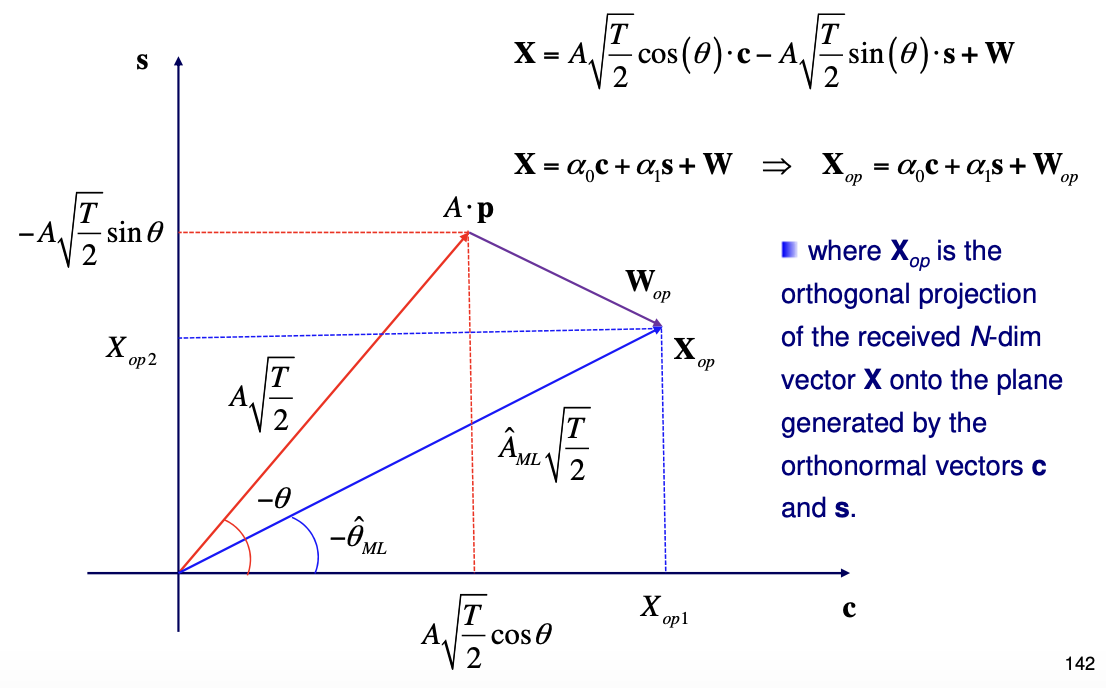
\includegraphics[width=0.75\linewidth]{Image/pdf 4/25.Rapp_2.png}
        \label{fig:placeholder}
    \end{figure}
    \[
\begin{cases}
A = \sqrt{\frac{2}{T}} \|\mathbf{A \cdot p}\|, \quad\\
  \theta = -\angle (\mathbf{A \cdot p}) 
\end{cases}
\Rightarrow
\begin{cases}
\hat{A}_{ML} = \sqrt{\frac{2}{T}} \| \mathbf{x}_{op} \|, \quad\\
  \hat{\theta}_{ML} = -\angle \mathbf{x}_{op}
\end{cases}
\]
    \item Another interpretation of the ML estimators ad the DTFT of the data vector \textbf{x}:
\[
\begin{aligned}
Y &\triangleq \mathbf{c}^T \mathbf{x} - j \mathbf{s}^T \mathbf{x} \\[2ex]
  &= \sqrt{\frac{2}{N}} \sum_{i=0}^{N-1} x_i \cos(2\pi F_0 i)
     - j \sqrt{\frac{2}{N}} \sum_{i=0}^{N-1} x_i \sin(2\pi F_0 i) \\[2ex]
  &= \sqrt{\frac{2}{N}} \sum_{i=0}^{N-1} x_i \left[ \cos(2\pi F_0 i) - j\sin(2\pi F_0 i) \right] \\[2ex]
  &= \sqrt{\frac{2}{N}} \sum_{i=0}^{N-1} x_i e^{-j 2\pi F_0 i} \\[2ex]
  &= \sqrt{\frac{2}{N}} \cdot DTFT\big\{ \mathbf{x} \big\} \Big|_{F=F_0}
\end{aligned}
\]
    \item Hence, the ML estimators coincide with the MM.
\begin{figure}[H]
    \centering
    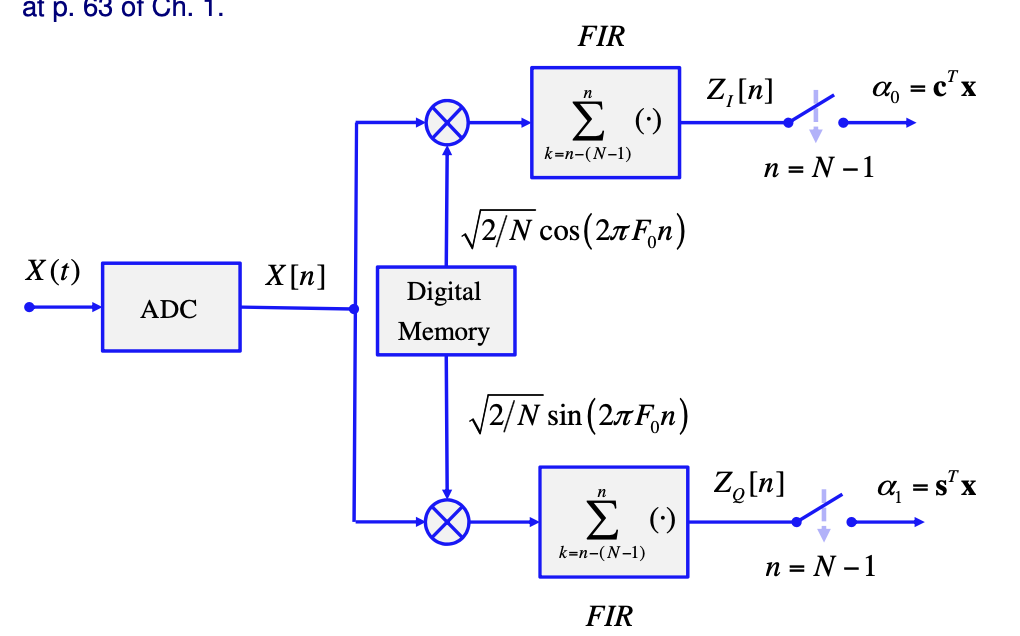
\includegraphics[width=0.6\linewidth]{Image/pdf 4/26.Block_diag_1.png}
    \label{fig:placeholder}
\end{figure}
    \item Alternative approach: \textbf{correlator} structure that uses an analog \textbf{moving window integrator (MWI)}:
    \begin{figure}[H]
        \centering
        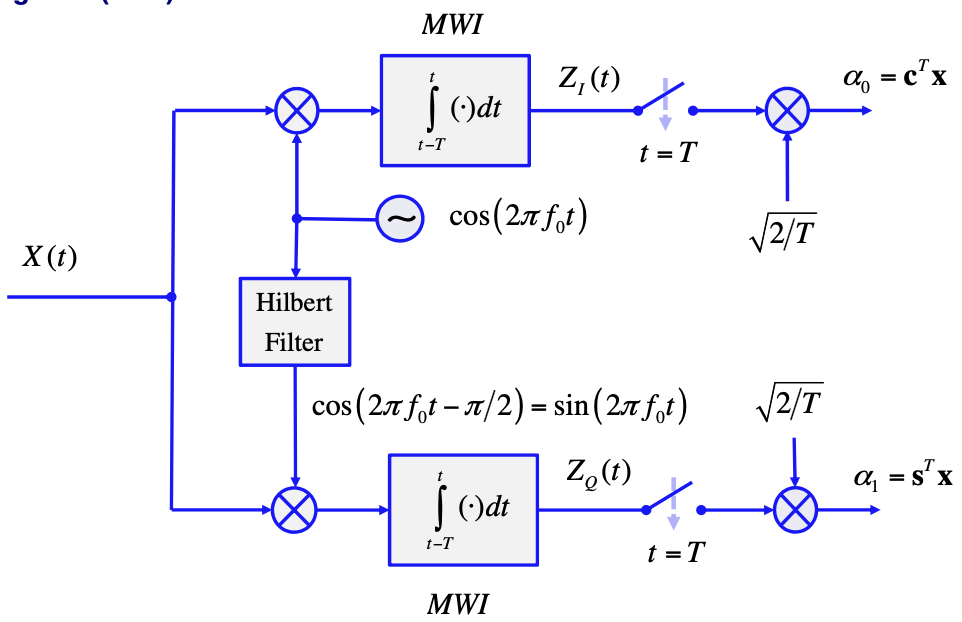
\includegraphics[width=0.6\linewidth]{Image/pdf 4/27.Block_diag_2.png}
        \label{fig:placeholder}
    \end{figure}
    \item \textbf{Performance of the ML estimators}:
\[
\hat{A}_{ML} = \sqrt{2B} \cdot \frac{2}{N} \sum_{i=0}^{N-1} x_i \cos \left(2\pi F_0 i + \hat{\theta}_{ML}\right)
\]
\[
= \sqrt{2B} \cdot \frac{2}{N} \sum_{i=0}^{N-1} x_i \cos(2\pi F_0 i) \cos(\hat{\theta}_{ML})
- \sqrt{2B} \cdot \frac{2}{N} \sum_{i=0}^{N-1} x_i \sin(2\pi F_0 i) \sin(\hat{\theta}_{ML})
\]
\[
= \sqrt{2B} \sqrt{ \frac{2}{N} } \left( \mathbf{c}^T \mathbf{x} \cos(\hat{\theta}_{ML}) - \mathbf{s}^T \mathbf{x} \sin(\hat{\theta}_{ML}) \right)
\]
\[
\underset{N=2BT}{=} \sqrt{\frac{2}{T}} \left( (\mathbf{c}^T \mathbf{x}) \cos(\hat{\theta}_{ML}) - (\mathbf{s}^T \mathbf{x}) \sin(\hat{\theta}_{ML}) \right)
\]
    \item \textbf{X} is a Gaussian distributed random vector, so \(\mathbf{c}^T\mathbf{X}\) and \(\mathbf{s}^T\mathbf{X}\) are two jointly Gaussian r.v.'s:
    \[
\mathbf{X} = A \cdot \mathbf{p}(\theta) + \mathbf{W} \in \mathcal{N}\left(A \cdot \mathbf{p}(\theta),\, \sigma_W^2 \mathbf{I} \right)
\]
    \item Let us derive the joint pdf of \(\mathbf{c}^T\mathbf{X}\) and \(\mathbf{s}^T\mathbf{X}\):
    \[
\begin{aligned}
\mathbf{X} &= A\sqrt{\frac{T}{2}}\cos\theta\cdot\mathbf{c} - A\sqrt{\frac{T}{2}}\sin\theta\cdot\mathbf{s} + \mathbf{W} \\[2ex]
\mathbf{c}^T\mathbf{X} 
    &= A\sqrt{\frac{T}{2}}\cos\theta \cdot \mathbf{c}^T\mathbf{c} 
     - A\sqrt{\frac{T}{2}}\sin\theta \cdot \mathbf{c}^T\mathbf{s} + \mathbf{c}^T\mathbf{W} \\ 
    &= A\sqrt{\frac{T}{2}}\cos\theta + \mathbf{c}^T\mathbf{W} \\[2ex]
\mathbf{s}^T\mathbf{X}
    &= A\sqrt{\frac{T}{2}}\cos\theta \cdot \mathbf{s}^T\mathbf{c} 
     - A\sqrt{\frac{T}{2}}\sin\theta \cdot \mathbf{s}^T\mathbf{s} + \mathbf{s}^T\mathbf{W} \\
    &= -A\sqrt{\frac{T}{2}}\sin\theta + \mathbf{s}^T\mathbf{W} \\[2ex]
E\left\{\mathbf{c}^T\mathbf{X}\right\} &= A\sqrt{\frac{T}{2}}\cos\theta, \qquad
E\left\{\mathbf{s}^T\mathbf{X}\right\} = -A\sqrt{\frac{T}{2}}\sin\theta
\end{aligned}
\]
\[
\begin{aligned}
\mathrm{var}\left\{ \mathbf{c}^T\mathbf{X} \right\} 
    &= \mathrm{var}\left\{ \mathbf{c}^T\mathbf{W} \right\} 
     = E\left\{ \mathbf{c}^T \mathbf{W} (\mathbf{c}^T\mathbf{W})^{T}\right\} 
     = E\left\{ \mathbf{c}^T \mathbf{W} \mathbf{W}^T \mathbf{c}\right\} \\[2ex]
    &= \mathbf{c}^T E\left\{ \mathbf{W} \mathbf{W}^T \right\} \mathbf{c} 
     = \mathbf{c}^T \left( \sigma_w^2 \mathbf{I} \right) \mathbf{c}
     = \sigma_w^2 \mathbf{c}^T \mathbf{c}
     = \sigma_w^2 
     = \frac{N_0}{2} \\[3ex]
\mathrm{var}\left\{ \mathbf{s}^T\mathbf{X} \right\}
    &= \mathrm{var}\left\{ \mathbf{s}^T\mathbf{W} \right\}
     = \frac{N_0}{2} \\[3ex]
\mathrm{cov}\left\{ \mathbf{c}^T\mathbf{X}, \mathbf{s}^T\mathbf{X} \right\}
    &= E\left\{ \mathbf{c}^T \mathbf{W} (\mathbf{s}^T \mathbf{W})^T \right\}
     = \mathbf{c}^T E\left\{ \mathbf{W} \mathbf{W}^T \right\} \mathbf{s} 
     = \mathbf{c}^T \left( \sigma_w^2 \mathbf{I} \right) \mathbf{s} \\ 
    &= \sigma_w^2 \mathbf{c}^T \mathbf{s}
     = 0
\end{aligned}
\]
    \item Hence, \(\mathbf{c}^T\mathbf{X}\) and \(\mathbf{s}^T\mathbf{X}\) are uncorrelated, and since they jointly Gaussian, they are also independent
    \item In summary:
\[
\mathbf{c}^T\mathbf{X} \in \mathcal{N}\left( 
    A\sqrt{\frac{T}{2}}\cos\theta,\, \frac{N_0}{2} 
\right), 
\qquad
\mathbf{s}^T\mathbf{X} \in \mathcal{N}\left( 
    -A\sqrt{\frac{T}{2}}\sin\theta,\, \frac{N_0}{2} 
\right),
\]
\[
\text{mutually independent}
\]
    \item The ML estimates of \(A\) and \(\theta\) are obtained by applying the \textbf{Fundamental Theorem of transformation of random variables} to this transformation of two jointly Gaussian r.v's:\\
    In practice, it is the well-known transformation from Cartesian to Polar coordinates.
    \item Skipping the details of the derivation, the ML estimate of \(A\) is \textbf{Rice} distributed:
    \[
f_{\hat{A}_{ML}}(a) = \frac{a}{N_0/T} \exp\left( -\frac{a^2 + A^2}{2N_0/T} \right) I_0\left(\frac{aA}{N_0/T}\right) u(a)
\]
    \item Where \(I_0(.)\) is the modified Bessel function of first kind of zero order.\\
    It is a biparametric pdf which depends on the parameters \(A\) and \(N_0/T\).\\
    When \(v=A=0\), we get the Rayleigh distribution, since \(I_0(0)=1\):
    \[
    f_{\hat{A}_{ML}}(a) = \frac{a}{N_0/T}\,\exp\left(-\frac{a^2}{2N_0/T}\right) u(a)
    \]
    and the pdf of the ML estimate of the phase is uniformly distributed in \([-\pi,+\pi)\).
    \item It can be shown that: \(\text{var}\{\hat{A}_{ML}\}\propto\frac{N_0}{T}\)
    \item When \(A^2T/2N_0>1\), that means high output Signal-to-Noise power Ratio (\(SNR_{out}\)), the Rice pdf tends to a Gaussian pdf.
    \[
    \lim_{T \to \infty} \frac{N_0}{T} = 0
    \quad \Rightarrow \quad
    \lim_{T \to \infty} f_{\hat{A}_{ML}}(a) = \delta(a-A)
    \quad \text{so the estimator is consistent}
    \]
    \[
    \text{where} \qquad SNR_{out} \triangleq \frac{A^2 T}{2 N_0}
    \]
    \item The \textbf{Input Signal to Noise power Ratio} (\(SNR_{in}\)) is the \(SNR\) after the digital conversion, i.e. calculated for the image vector \textbf{X}:

    \[
\begin{aligned}
\mathbf{X} &= A\cdot\mathbf{p}(\theta) + \mathbf{W}
= A\sqrt{\frac{T}{2}}\cos(\theta)\cdot\mathbf{c} - A\sqrt{\frac{T}{2}}\sin(\theta)\cdot\mathbf{s} + \mathbf{W} \\[2ex]
SNR_{in} &= \frac{\left\|A\sqrt{\frac{T}{2}}\cos(\theta)\cdot\mathbf{c} - A\sqrt{\frac{T}{2}}\sin(\theta)\cdot\mathbf{s}\right\|^2}{E\{\|\mathbf{W}\|^2\}}
= \frac{A^2T}{2} \cdot \frac{1}{N(N_0/2)} = \frac{A^2 T}{2N_0} \cdot \frac{2}{N} \\[2ex]
&= \frac{A^2 T}{2N_0} \cdot \frac{2}{2BT}
= \frac{A^2}{2N_0 B}\end{aligned} \]
\[
\left\| A\sqrt{\frac{T}{2}}\cos(\theta)\cdot\mathbf{c} - A\sqrt{\frac{T}{2}}\sin(\theta)\cdot\mathbf{s}\right\|^2
    = \left(A\sqrt{\frac{T}{2}}\cos(\theta)\right)^2 + \left(-A\sqrt{\frac{T}{2}}\sin(\theta)\right)^2
    = \frac{A^2 T}{2}
\]
    \item The \textbf{output Signal to Noise power Ratio} (\(SNR_{out}\)) is the \(SNR\) after the two matched filters that implement the orthogonal projection of \textbf{X} onto the plane generated by the vectors \textbf{c} and \textbf{s}, i.e. onto the signal subspace.
\[
\begin{aligned}
\mathbf{X}_{op} &= A\cdot\mathbf{p}(\theta) + \mathbf{W}_{op}
= A\sqrt{\frac{T}{2}}\cos(\theta)\cdot\mathbf{c} - A\sqrt{\frac{T}{2}}\sin(\theta)\cdot\mathbf{s} + \mathbf{W}_{op} \\[2ex]
SNR_{out} &= \frac{ \left\| A\sqrt{\frac{T}{2}}\cos(\theta)\cdot\mathbf{c}
              - A\sqrt{\frac{T}{2}}\sin(\theta)\cdot\mathbf{s} \right\|^2 }
             { E\{ \|\mathbf{W}_{op}\|^2 \} }
= \frac{A^2 T}{2} \cdot \frac{1}{2(N_0/2)} = \frac{A^2 T}{2 N_0} \\[3ex]
E\left\{\|\mathbf{W}_{op}\|^2\right\}
 &= E\left\{ \left( \mathbf{c}^T\mathbf{W} \right)^2 + \left( \mathbf{s}^T\mathbf{W} \right)^2 \right\}
= 2 \cdot \frac{N_0}{2}
\end{aligned}
\]
    \item The \textbf{Processing Gain (PG)} is immediately obtained:

    \[
SNR_{in} = \frac{A^2}{2BN_0},\qquad
SNR_{out} = \frac{A^2 T}{2N_0}
\;\;\longrightarrow\;\;
PG = \frac{SNR_{out}}{SNR_{in}} = BT = \frac{N}{2}
\]
    \item Note that the PG is one half the PG in the previous case, when the signal shape was perfectly known, i.e. known \(\theta\).
    \item This should not be a surprise since now the Signal of Interest (SOI) belongs to a 2D subspace instead of a 1D subspace, so there is more uncertainty about the SOI.
    \item The \textbf{Rice} distribution with parameters (\(A,N_0/T\)) has moments of even order that can be expressed as a polynomials in \(A\) and \(N_0/T\), e.g. the \(2^{nd}\) order moment:
\[
E\left\{\hat{A}_{ML}^2\right\} = A^2 + \frac{2N_0}{T}
= A^2\left(1 + \frac{1}{SNR_{out}}\right),
\qquad
\text{where}\;\; SNR_{out} \triangleq \frac{A^2 T}{2N_0}
= \frac{N}{2}SNR_{in}
\]
    \item The odd order moments cannot be expressed in closed form; they can be expressed as a function of the generalized Laguerre polynomials, e.g. the mean:

    \item Hence, it is not possible to calculate bias and MSE in closed form.
    \begin{figure}[H]
        \centering
        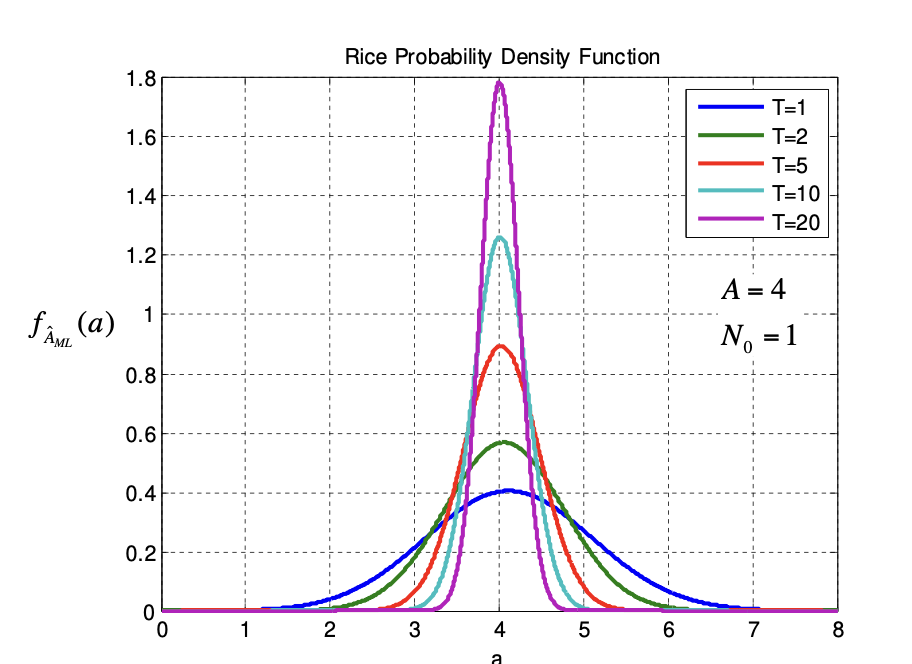
\includegraphics[width=0.6\linewidth]{Image/pdf 4/28.Rice_distribution.png}
        \label{fig:placeholder}
    \end{figure}
    \begin{figure}[H]
    \centering
    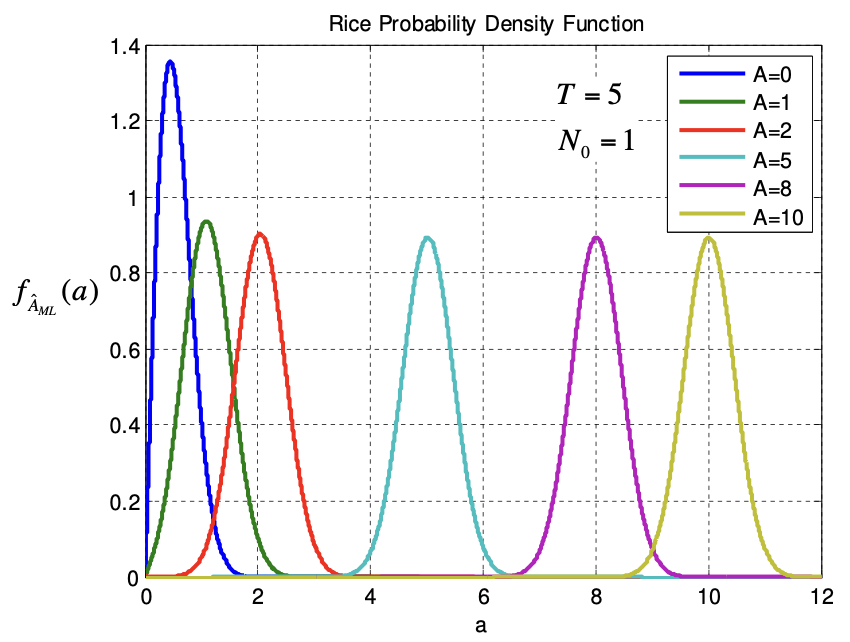
\includegraphics[width=0.6\linewidth]{Image/pdf 4/29.Rice_2.png}
    \label{fig:placeholder}
    \end{figure}
    \item \textbf{Cramèr-Rao lower Bound (CRB)} on amplitude and phase and comparison of the MSE (derived by Monte Carlo simulation) with the CRB:
    \[
\begin{aligned}
\mathbf{C}_\theta &= E \left\{ \begin{pmatrix} \hat{\theta} - \theta \\ \hat{A} - A \end{pmatrix} \begin{pmatrix} \hat{\theta} - \theta \\ \hat{A} - A \end{pmatrix}^T \right\} 
= E\left\{
\begin{bmatrix}
\hat{A} - A \\ \hat{\theta} - \theta
\end{bmatrix}
\begin{bmatrix}
\hat{A} - A & \hat{\theta} - \theta
\end{bmatrix}
\right\} \\[2ex]
&= 
\begin{bmatrix}
E\left\{(\hat{A}-A)^2\right\} & E\left\{ (\hat{A}-A)(\hat{\theta}-\theta) \right\} \\
E\left\{ (\hat{A}-A)(\hat{\theta}-\theta) \right\} & E\left\{ (\hat{\theta}-\theta)^2 \right\}
\end{bmatrix}
\end{aligned}
\]

\[
\mathbf{C}_\theta \ge CRB(A, \theta) = \mathbf{I}^{-1}(A, \theta)
= \left[
\begin{matrix}
- E\left\{\frac{\partial^2 \ln L(A, \theta)}{\partial A^2}\right\} & -E\left\{ \frac{\partial^2 \ln L(A, \theta)}{\partial A \partial \theta} \right\} \\
- E\left\{ \frac{\partial^2 \ln L(A, \theta)}{\partial \theta \partial A} \right\} & -E\left\{ \frac{\partial^2 \ln L(A, \theta)}{\partial \theta^2} \right\}
\end{matrix}
\right]^{-1}
\]

    
    \item We have already derived the first order derivatives of the log-likelihood function with respect to the unknown parameters \(A\) and \(\theta\):
\[
\left\{
\begin{aligned}
\frac{\partial \ln L(A, \theta)}{\partial A} &=
- \frac{A N}{N_0 2B}
+ \frac{2}{N_0 \sqrt{2B}} \sum_{i=0}^{N-1} x_i \cos\left(2\pi F_0 i + \theta\right)
\\[2ex]
\frac{\partial \ln L(A, \theta)}{\partial \theta} &=
- \frac{2A}{N_0 \sqrt{2B}}
\sum_{i=0}^{N-1} x_i \sin\left(2\pi F_0 i + \theta\right)
\end{aligned}
\right.
\]
    \item The 2nd order derivatives and the \textbf{Fisher Information Matrix (FIM)} elements are :
    \[
\frac{\partial^2 \ln L(A, \theta)}{\partial A^2} =
- \frac{N}{N_0 2B}
= -\frac{T}{N_0}
\;\; \rightarrow \;\;
I_{11} = -E\left\{ \frac{\partial^2 \ln L(A, \theta)}{\partial A^2} \right\}
= \frac{T}{N_0}
\]
\[
\frac{\partial^2 \ln L(A, \theta)}{\partial \theta \partial A}
= \frac{\partial^2 \ln L(A, \theta)}{\partial A \partial \theta}
= -\frac{2}{N_0 \sqrt{2B}} \sum_{i=0}^{N-1} x_i \sin(2\pi F_0 i + \theta)
\]
\[
= -\frac{2}{N_0 \sqrt{2B}}
\left[
\sum_{i=0}^{N-1} x_i \sin(2\pi F_0 i) \cos(\theta)
+ \sum_{i=0}^{N-1} x_i \cos(2\pi F_0 i) \sin(\theta)
\right]
\]
\[
= -\frac{2}{N_0 \sqrt{2B}} \sqrt{\frac{N}{2}}
\left[
\mathbf{s}^T \mathbf{X} \cos(\theta)
+ \mathbf{c}^T \mathbf{X} \sin(\theta)
\right]
\]
\[
I_{21} = I_{12}
= -E\left\{ \frac{\partial^2 \ln L(A, \theta)}{\partial A \partial \theta} \right\}
= \frac{2}{N_0 \sqrt{2B}} \sqrt{\frac{N}{2}}
\left[ E\{\mathbf{s}^T\mathbf{X}\} \cos(\theta) + E\{\mathbf{c}^T\mathbf{X}\} \sin(\theta) \right]
\]
\[
= \frac{2}{N_0 \sqrt{2B}}
\sqrt{\frac{N}{2}}
\left[
- A\sqrt{\frac{T}{2}} \sin(\theta) \cos(\theta)
+ A\sqrt{\frac{T}{2}} \cos(\theta) \sin(\theta)
\right]
= 0
\]
\[
\text{where we used the results:}
\quad
E\{ \mathbf{c}^T \mathbf{X} \}
= A\sqrt{\frac{T}{2}} \cos(\theta),
\qquad
E\{ \mathbf{s}^T \mathbf{X} \}
= -A\sqrt{\frac{T}{2}} \sin(\theta)
\]
    \[
\begin{aligned}
\frac{\partial^2 \ln L(A, \theta)}{\partial \theta^2} &=
- \frac{2A}{N_0 \sqrt{2B}} \sum_{i=0}^{N-1} x_i \cos(2\pi F_0 i + \theta)
\\[2ex]
&= - \frac{2A}{N_0 \sqrt{2B}}
\left[
\sum_{i=0}^{N-1} x_i \cos(2\pi F_0 i) \cos(\theta)
- \sum_{i=0}^{N-1} x_i \sin(2\pi F_0 i) \sin(\theta)
\right]\\[2ex]
&= - \frac{2A}{N_0 \sqrt{2B}} \sqrt{\frac{N}{2}}
\left[
\mathbf{c}^T \mathbf{X} \cos(\theta)
- \mathbf{s}^T \mathbf{X} \sin(\theta)
\right]\\[2ex]
I_{22} &= -E\left\{ \frac{\partial^2 \ln L(A, \theta)}{\partial \theta^2} \right\}
= \frac{2A}{N_0 \sqrt{2B}} \sqrt{\frac{N}{2}}
\left[
E \{ \mathbf{c}^T \mathbf{X} \} \cos(\theta)
- E \{ \mathbf{s}^T \mathbf{X} \} \sin(\theta)
\right]\\[2ex]
&= \frac{2A}{N_0 \sqrt{2B}} \sqrt{\frac{N}{2}}
\left[
A \sqrt{\frac{T}{2}} \cos(\theta) \cos(\theta)
+ A \sqrt{\frac{T}{2}} \sin(\theta) \sin(\theta)
\right] = \frac{2A}{N_0 \sqrt{2B}} \sqrt{\frac{N}{2}} A \sqrt{\frac{T}{2}}\\[2ex]
&= \frac{2A^2}{N_0 \sqrt{2B}} \sqrt{\frac{BT}{2}} \sqrt{\frac{T}{2}}
= \frac{A^2 T}{N_0}
\end{aligned}
\]
    \item hence, the FIM is diagonal :
    \[
\mathbf{I}(A, \theta) = 
\begin{bmatrix}
\frac{T}{N_0} & 0 \\
0 & \frac{T A^2}{N_0}
\end{bmatrix}
\implies
\mathbf{I}^{-1}(A, \theta) = 
\begin{bmatrix}
\frac{N_0}{T} & 0 \\
0 & \frac{N_0}{T A^2}
\end{bmatrix}
\]
    \item The CRB's on the estimation of amplitude and phase are:
    \[
\text{var}\left\{\hat{A}\right\} \geq CRB(A) = \frac{N_0}{T}
\]
\[
\text{var}\left\{\hat{\theta}\right\} \geq CRB(\theta) = \frac{N_0}{A^2 T} = \frac{N_0}{2 E_s}
\]
\[
E_s = A^2 E_p = \frac{A^2 T}{2}
\]
    \item The CRB's can be expressed in terms of \(SNR_{in}\) or \(SNR_{out}\):
    \[
SNR_{in} = \frac{A^2}{2 B N_0}, \qquad
SNR_{out} = \frac{A^2 T}{2 N_0} = \frac{N}{2} SNR_{in}
\]

    \item The two CRBs are given by:
    \[
\left\{
\begin{aligned}
    &\text{var}\left\{\hat{A}\right\} \geq CRB(A) = \frac{N_0}{T}
    = \frac{A^2}{2 \cdot SNR_{out}}
    = \frac{A^2}{N \cdot SNR_{in}} \\[2em]
    &\text{var}\left\{\hat{\theta}\right\} \geq CRB(\theta) = \frac{N_0}{A^2 T}
    = \frac{N_0}{2 E_s}
    = \frac{1}{2 \cdot SNR_{out}}
    = \frac{1}{N \cdot SNR_{in}}
\end{aligned}
\right.
\]
    \item Due to the asymptotic properties of all ML estimators (under some mild conditions), we have that when the observation interal \(T\) goes to infinity, i.e. \(T\rightarrow+\infty\), or equivalently \(SNR_{out}\rightarrow+\infty\), we have:
    \[
\left\{
\begin{aligned}
    &\hat{A}_{ML} \; \overset{a}{\in} \mathcal{N}\left(A, \frac{N_0}{T}\right) \equiv \mathcal{N}\left(A, \frac{A^2}{2 \cdot SNR_{out}}\right) \\[2em]
    &\hat{\theta}_{ML} \; \overset{a}{\in} \mathcal{N}\left(\theta, \frac{N_0}{A^2 T}\right) \equiv \mathcal{N}\left(\theta, \frac{1}{2 \cdot SNR_{out}}\right)
\end{aligned}
\right.
\]
    \item I.e. the estimators are asymptotically efficient, asymptotically unbiased and consistent, since MSE \(\rightarrow 0\) when \(T\rightarrow\infty\), i.e. \(SNR_{out}\rightarrow\infty\).
\begin{figure}[H]
    \centering
    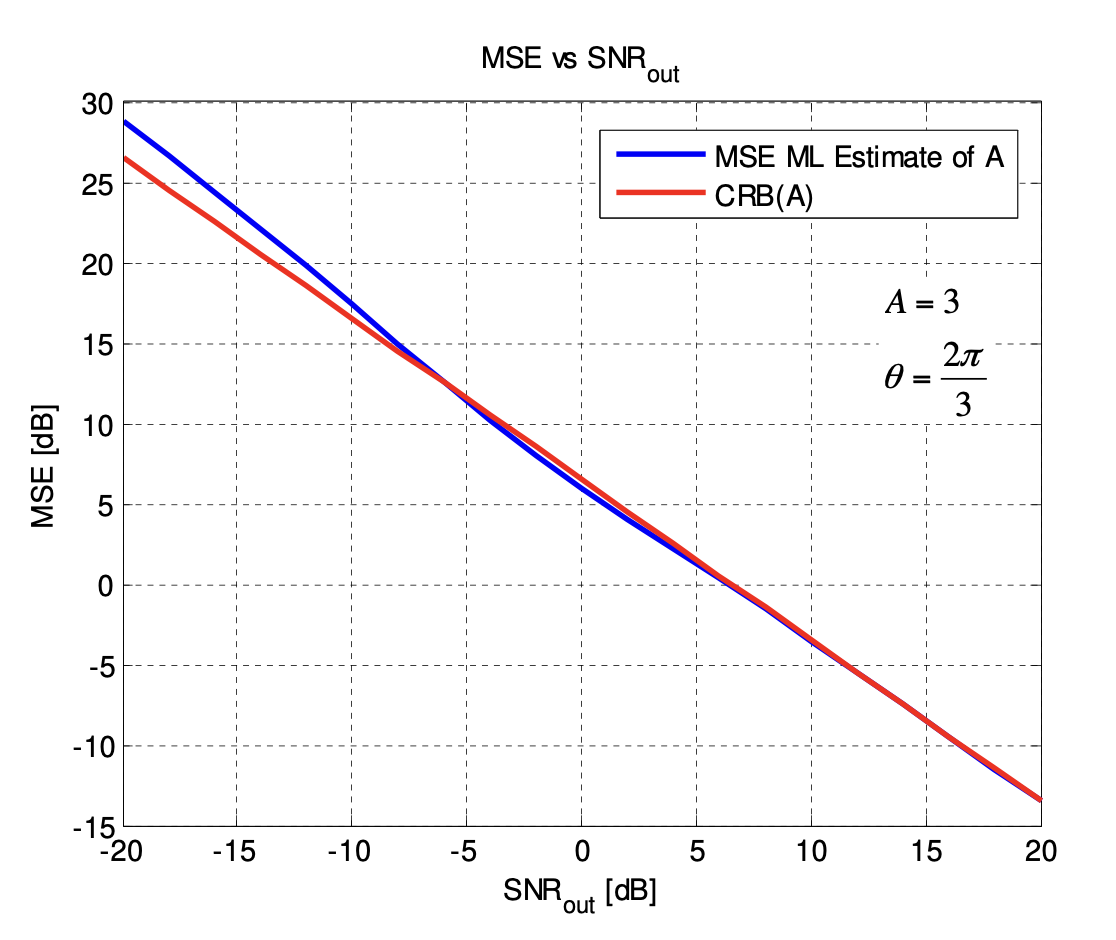
\includegraphics[width=0.55\linewidth]{Image/pdf 4/30.SNR_vs_MSE_1.png}
    \label{fig:placeholder}
\end{figure}
\begin{figure}[H]
    \centering
    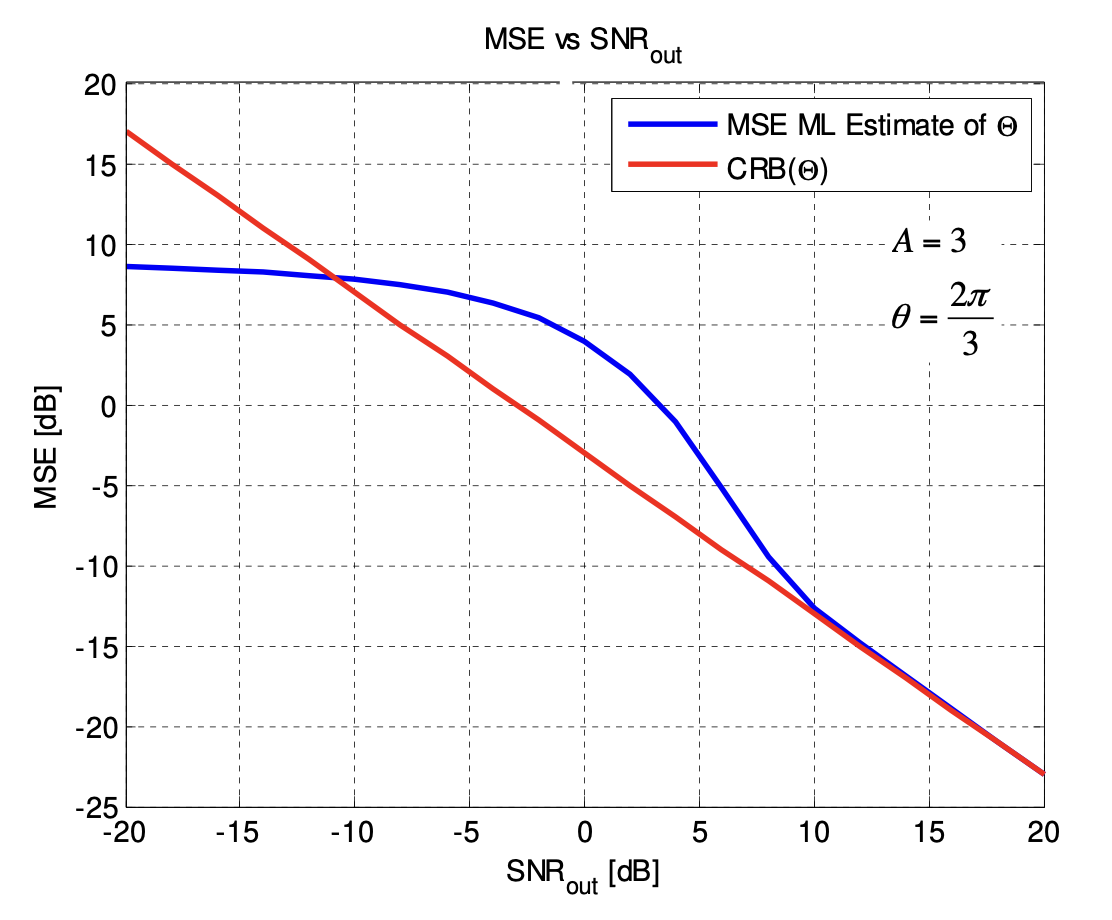
\includegraphics[width=0.55\linewidth]{Image/pdf 4/31.SNR_vs_MSE_2.png}
    \label{fig:placeholder}
\end{figure}
    \item Note that the plot is in \(dB\) on both scales, that's why the CRB curves are lines with slope \(-1\):
    \[
\begin{aligned}
    CRB(A)_{dB} &= 10\log_{10} CRB(A) = 10\log_{10}\left(\frac{A^2}{2SNR_{out}}\right) \\
    &= 20\log_{10}(A) - 10\log_{10}(2) - 10\log_{10}(SNR_{out}) \\
    &= 20\log_{10}(A) - 10\log_{10}(2) - SNR_{out,dB}
\end{aligned}
\]

\[
\begin{aligned}
    CRB(\theta)_{dB} &= 10\log_{10} CRB(\theta) = 10\log_{10}\left(\frac{1}{2SNR_{out}}\right) \\
    &= -10\log_{10}(2) - 10\log_{10}(SNR_{out}) \\
    &= -10\log_{10}(2) - SNR_{out,dB}
\end{aligned}
\]
\begin{figure}[H]
    \centering
    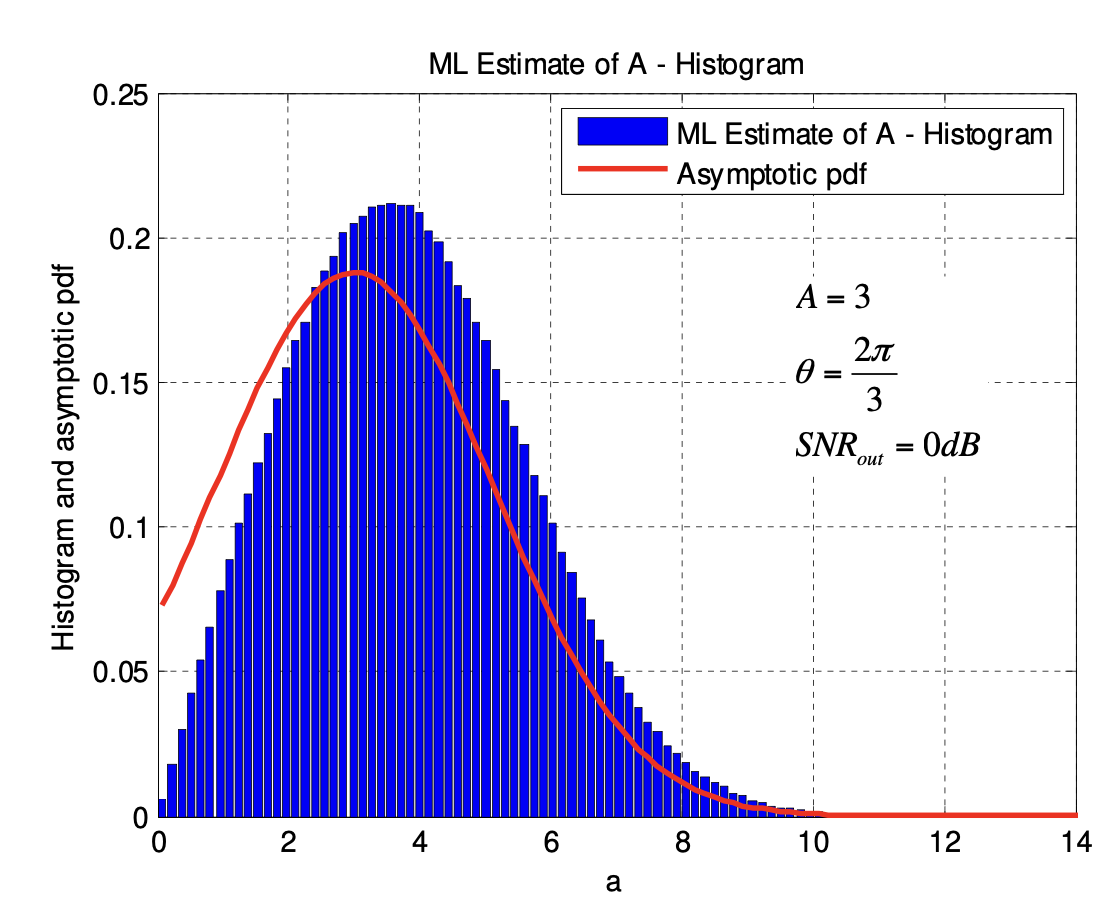
\includegraphics[width=0.5\linewidth]{Image/pdf 4/32.ML_estimate_1.png}
    \label{fig:placeholder}
\end{figure}
\begin{figure}[H]
    \centering
    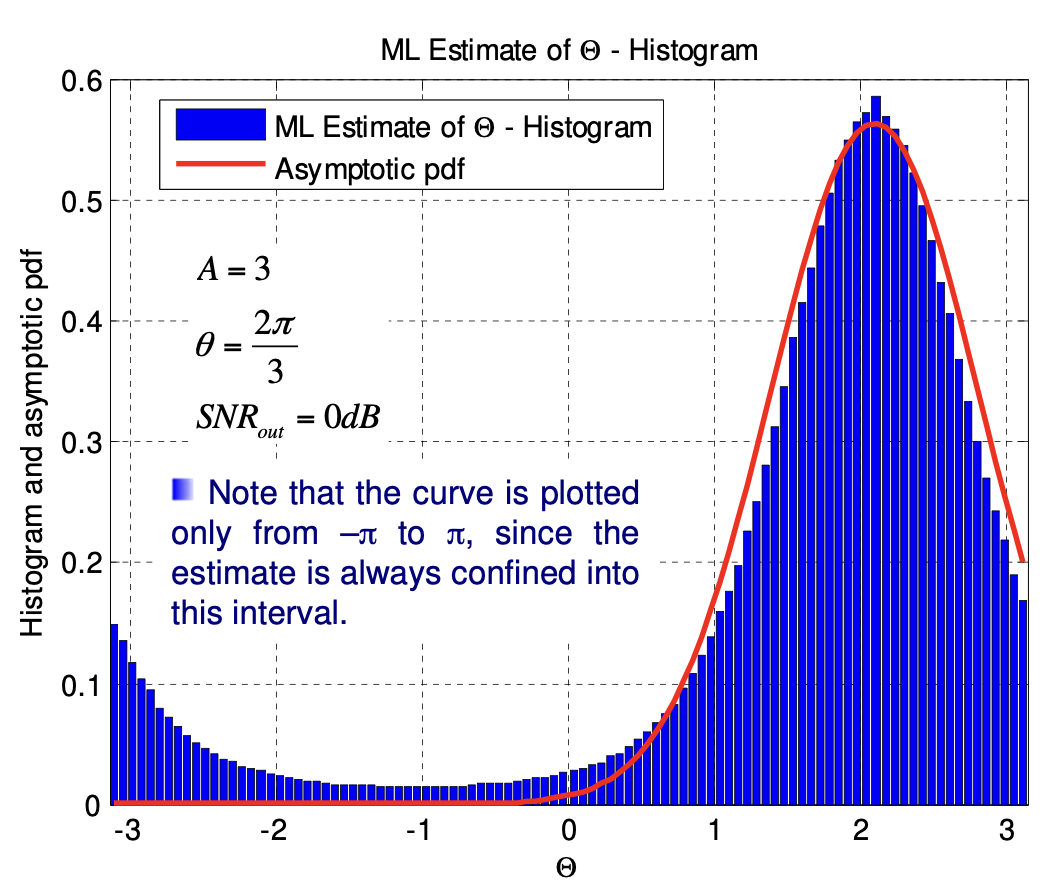
\includegraphics[width=0.5\linewidth]{Image/pdf 4/33.ML_estimate_2.png}
    \label{fig:placeholder}
\end{figure}
\begin{figure}[H]
    \centering
    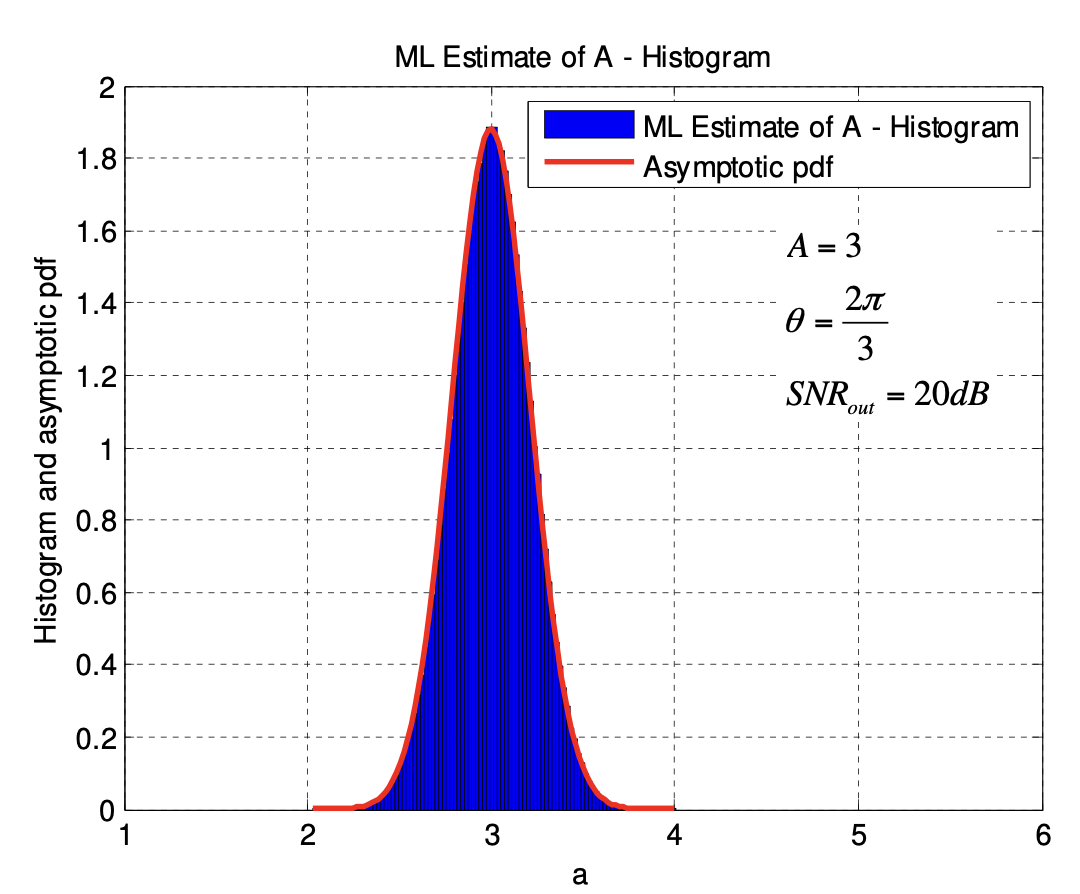
\includegraphics[width=0.5\linewidth]{Image/pdf 4/34.ML_estimate_3.png}
    \label{fig:placeholder}
\end{figure}
\begin{figure}[H]
    \centering
    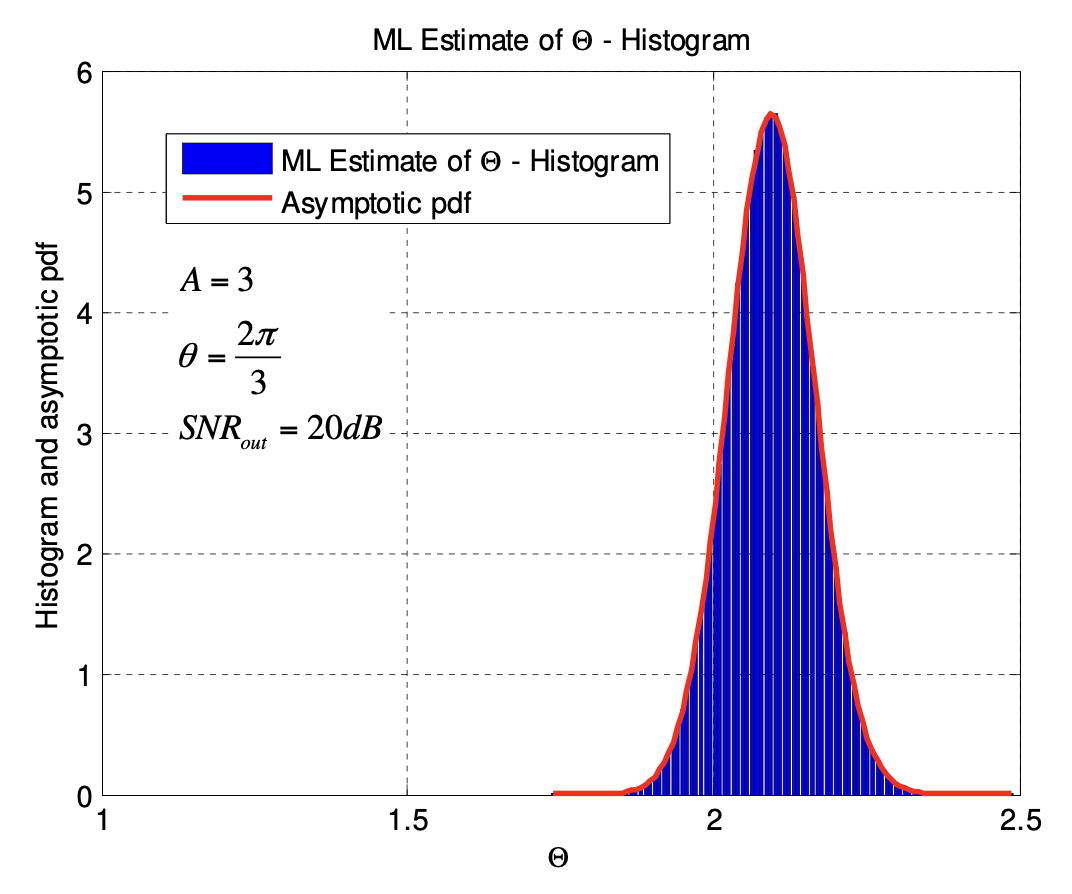
\includegraphics[width=0.5\linewidth]{Image/pdf 4/35.ML_estimate_4.png}
    \label{fig:placeholder}
\end{figure}
\end{itemize}
\subsection{ML estimate of the parameters of a Signal: Amplitude, Phase and Frequency}
\begin{itemize}
    \item Consider now the case when all the signal parameters (amplitude, phase and frequency) are unknown.
    \item If the frequency \(F_0\) is also unknown, the previously derived algorithm cannot be implemented.
\begin{figure}[H]
    \centering
    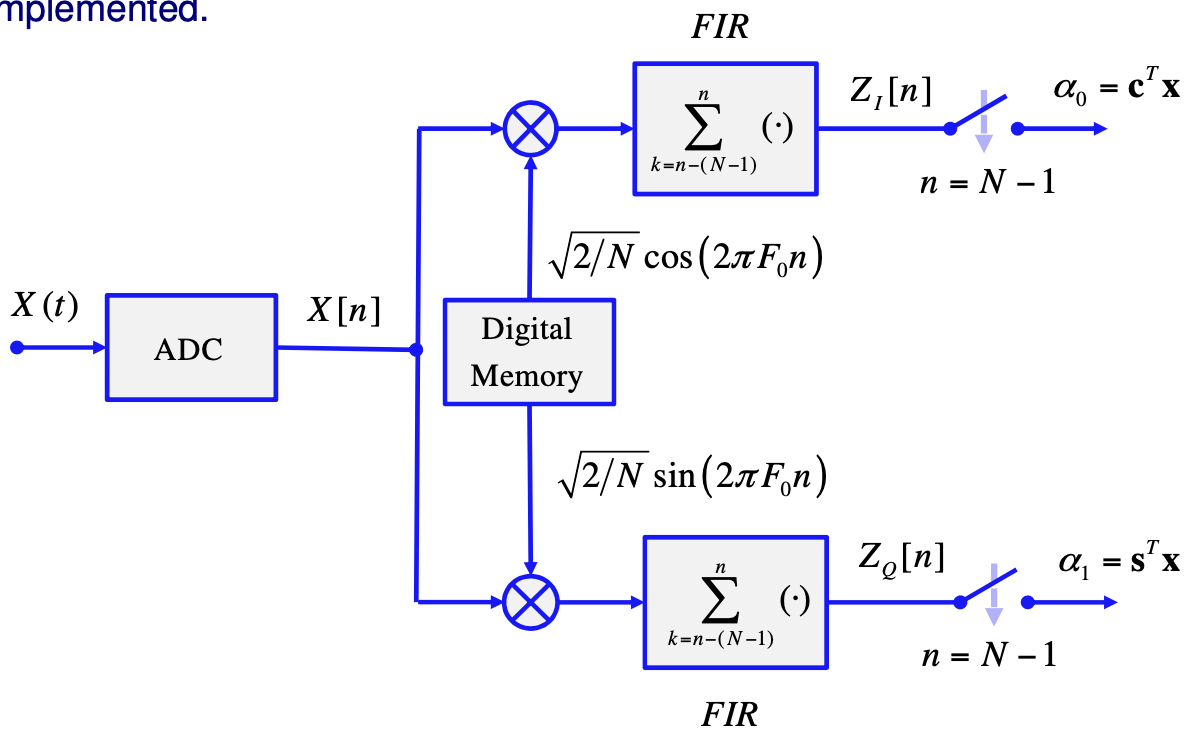
\includegraphics[width=0.5\linewidth]{Image/pdf 4/36.Block_diag.png}
    \label{fig:placeholder}
\end{figure}

    \item The observed data vector \textbf{X} is exactly yhe same as before:
\[
\textbf{X} \text{ image of } X(t) \text{ for } t \in [0, T)
\]

\[
\textbf{X} = 
\begin{bmatrix}
X_0 \\
X_1 \\
\vdots \\
X_{N-1}
\end{bmatrix}
= A \cdot \mathbf{p}(\theta) + \mathbf{W} =
\begin{bmatrix}
\frac{A}{\sqrt{2B}} \cos(\theta) \\
\frac{A}{\sqrt{2B}} \cos(2\pi F_0 + \theta) \\
\vdots \\
\frac{A}{\sqrt{2B}} \cos(2\pi F_0 (N-1) + \theta)
\end{bmatrix}
+
\begin{bmatrix}
W_0 \\
W_1 \\
\vdots \\
W_{N-1}
\end{bmatrix}
\]

\[
\{ W_i \}_{j=0}^{N-1} \text{ IID}, \quad W_i \in \mathcal{N}(0, \sigma_w^2), \quad \sigma_w^2 = \text{var}\{ W_j \} = \frac{N_0}{2}
\]

\[
X_i \in \mathcal{N}\left( A \cdot p_i(\theta), \sigma_w^2 \right)
\]

\[
F_0 \triangleq \frac{f_0}{2B} \qquad \text{Digital Frequency - Nyquist Sampling} \qquad 0 < F_0 < \frac{1}{2}
\]


    \item The \textbf{log-likehood function (log-lf)} is also the same as before:
\[
\ln L(A, \theta, F_0) = \ln f_X(\mathbf{x}; A, \theta, F_0)
= \kappa - \frac{A^2}{N_0 2B} \cdot \frac{N}{2}
+ \frac{2A}{N_0 \sqrt{2B}} \sum_{i=0}^{N-1} x_i \cos(2\pi F_0 i + \theta)
\]


    \item The jointly ML estimators of \(A\), \(\theta\) and \(F_0\) are obtained by jointly solving the likelihood equations, which are obtained by deriving the log-LF with respect to the three unknown parameters:
\[
\left\{
\begin{aligned}
    &\frac{\partial \ln L(A, \theta, F_0)}{\partial A} = 0 \\[2em]
    &\frac{\partial \ln L(A, \theta, F_0)}{\partial \theta} = 0 \\[2em]
    &\frac{\partial \ln L(A, \theta, F_0)}{\partial F_0} = 0
\end{aligned}
\right.
\]

    \item We have already solved the first two equations and derived the ML estimators of amplitude and phase when the signal frequency \(F_0\) is known.
    \item Note that the ML estimators of amplitude and phase are functions of \(F_0\):
    \[
\left\{
\begin{aligned}
    &\hat{A}_{ML}(F_0) = 
    \sqrt{\frac{2}{T}}
    \sqrt{
        \left(
            \sqrt{\frac{2}{N}} \sum_{i=0}^{N-1} x_i \cos\left(2\pi F_0 i\right)
        \right)^2
        +
        \left(
            \sqrt{\frac{2}{N}} \sum_{i=0}^{N-1} x_i \sin\left(2\pi F_0 i\right)
        \right)^2
    } \\[2em]
    &\hat{\theta}_{ML}(F_0) = -\arctan \left(
        \frac{
            \sqrt{\frac{2}{N}} \sum_{i=0}^{N-1} x_i \sin\left(2\pi F_0 i\right)
        }{
            \sqrt{\frac{2}{N}} \sum_{i=0}^{N-1} x_i \cos\left(2\pi F_0 i\right)
        }
    \right)
\end{aligned}
\right.
\]

    \item They are basically obtained by the modula and phase of the data vector DTFT calculated at the digital frequency \(F_0\):
\[
\left\{
\begin{aligned}
    &\hat{A}_{ML}(F_0) = 
    \sqrt{\frac{2}{T}} \sqrt{\frac{2}{N}} \left| DTFT\left\{\mathbf{x}\right\} \right|_{F=F_0} \\[2em]
    &\hat{\theta}_{ML}(F_0) = \angle DTFT\left\{\mathbf{x}\right\}\bigg|_{F=F_0}
\end{aligned}
\right.
\]
    \item We can insert the ML estimators of \(A\) and \(\theta\) in the log-LF and look for the maximum of the \textbf{"compressed" log-LF} with respect to the last unknown \(F_0\):
    \[
C(F_0) \triangleq \ln L\left(\hat{A}_{ML}(F_0), \hat{\theta}_{ML}(F_0), F_0\right)
= \kappa - \frac{\left(\hat{A}_{ML}(F_0)\right)^2}{N_0 2B} \cdot \frac{N}{2}
+ \frac{2\hat{A}_{ML}(F_0)}{N_0 \sqrt{2B}} \sum_{i=0}^{N-1} x_i \cos\left(2\pi F_0 i + \hat{\theta}_{ML}(F_0)\right)
\]

\[
\hat{F}_{0ML} = \underset{F_0}{\operatorname{argmax}}\, C(F_0) 
= \underset{F_0}{\operatorname{argmax}}\, \ln L\left(\hat{A}_{ML}(F_0), \hat{\theta}_{ML}(F_0), F_0\right)
= \underset{F_0}{\operatorname{argmax}} \left[
    -\frac{\left(\hat{A}_{ML}(F_0)\right)^2}{N_0 2B} \cdot \frac{N}{2}
    + \frac{2\hat{A}_{ML}(F_0)}{N_0 \sqrt{2B}} \sum_{i=0}^{N-1} x_i \cos\left(2\pi F_0 i + \hat{\theta}_{ML}(F_0)\right)
\right]
\]
    \item If we now recall that (see the derivative w.r.t \(A\)):

\[
\hat{A}_{ML} = \sqrt{2B} \cdot \frac{2}{N} \sum_{i=0}^{N-1} x_i \cos\left(2\pi F_0 i + \hat{\theta}_{ML}\right)
\longrightarrow
\sum_{i=0}^{N-1} x_i \cos\left(2\pi F_0 i + \hat{\theta}_{ML}\right)
= \frac{N}{2\sqrt{2B}} \hat{A}_{ML}
\]

\[
\begin{aligned}
    \hat{F}_{0ML} 
    &= \underset{F_0}{\operatorname{argmax}} \left[
        -\frac{\left(\hat{A}_{ML}(F_0)\right)^2}{N_0 2B} \cdot \frac{N}{2}
        + \frac{2\hat{A}_{ML}(F_0)}{N_0 \sqrt{2B}} \sum_{i=0}^{N-1} x_i \cos\left(2\pi F_0 i + \hat{\theta}_{ML}(F_0)\right)
    \right] \\[2em]
    &= \underset{F_0}{\operatorname{argmax}} \left[
        -\frac{\left(\hat{A}_{ML}(F_0)\right)^2}{N_0 2B} \cdot \frac{N}{2}
        + \frac{2\hat{A}_{ML}(F_0)}{N_0 \sqrt{2B}} \cdot \frac{N}{2\sqrt{2B}} \hat{A}_{ML}(F_0)
    \right] \\[2em]
    &= \underset{F_0}{\operatorname{argmax}} \left[
        \frac{N}{2} \cdot \frac{(\hat{A}_{ML}(F_0))^2}{N_0 2B}
    \right]
    = \underset{F_0}{\operatorname{argmax}} \left( \hat{A}_{ML}(F_0)^2 \right)
\end{aligned}
\]
    \item Hence, \(F_0\) is estimated as the location of the maximum of the observed data \textbf{Periodogram}. Once we have an estimate of \(F_0\), \(A\) and \(\theta\) are estimated as:
    

    \item The \textbf{Periodogram} is calculated via the efficient FFT with \underline{zero-padding} to \(N_{zp}\) points:
    \[
\hat{F}_{0ML} = \underset{F_0}{\operatorname{argmax}} \; \frac{1}{N} \left| \sum_{i=0}^{N_{zp}-1} x_i e^{-j2\pi F_0 i} \right|^2
= \underset{F_0}{\operatorname{argmax}} \; \frac{1}{N} \left| FFT\left\{\mathbf{x}\right\} \right|^2
\]
\[
\text{where} \quad x_i = 0 \quad \text{for } N \leq i \leq N_{zp}-1
\]
    \item The FFT is of order \(N_{zp}\), so the maximum is obtained with an accuracy (in the absence of noise) of \(1/N_{zp}\rightarrow\) there is a \underline{quantization error}. In the following we will investigate how the estimation accuracy is affected by the value of \(N_{zp}\).
    \item We will also observe the typical \textbf{threshold effect} for low SNR: below a threshold value of \(SNR\) the performance degrades very fast (we have the so called "catastrophic effect"). This is a typical behavior for any non linear estimator.
    \begin{figure}[H]
        \centering
        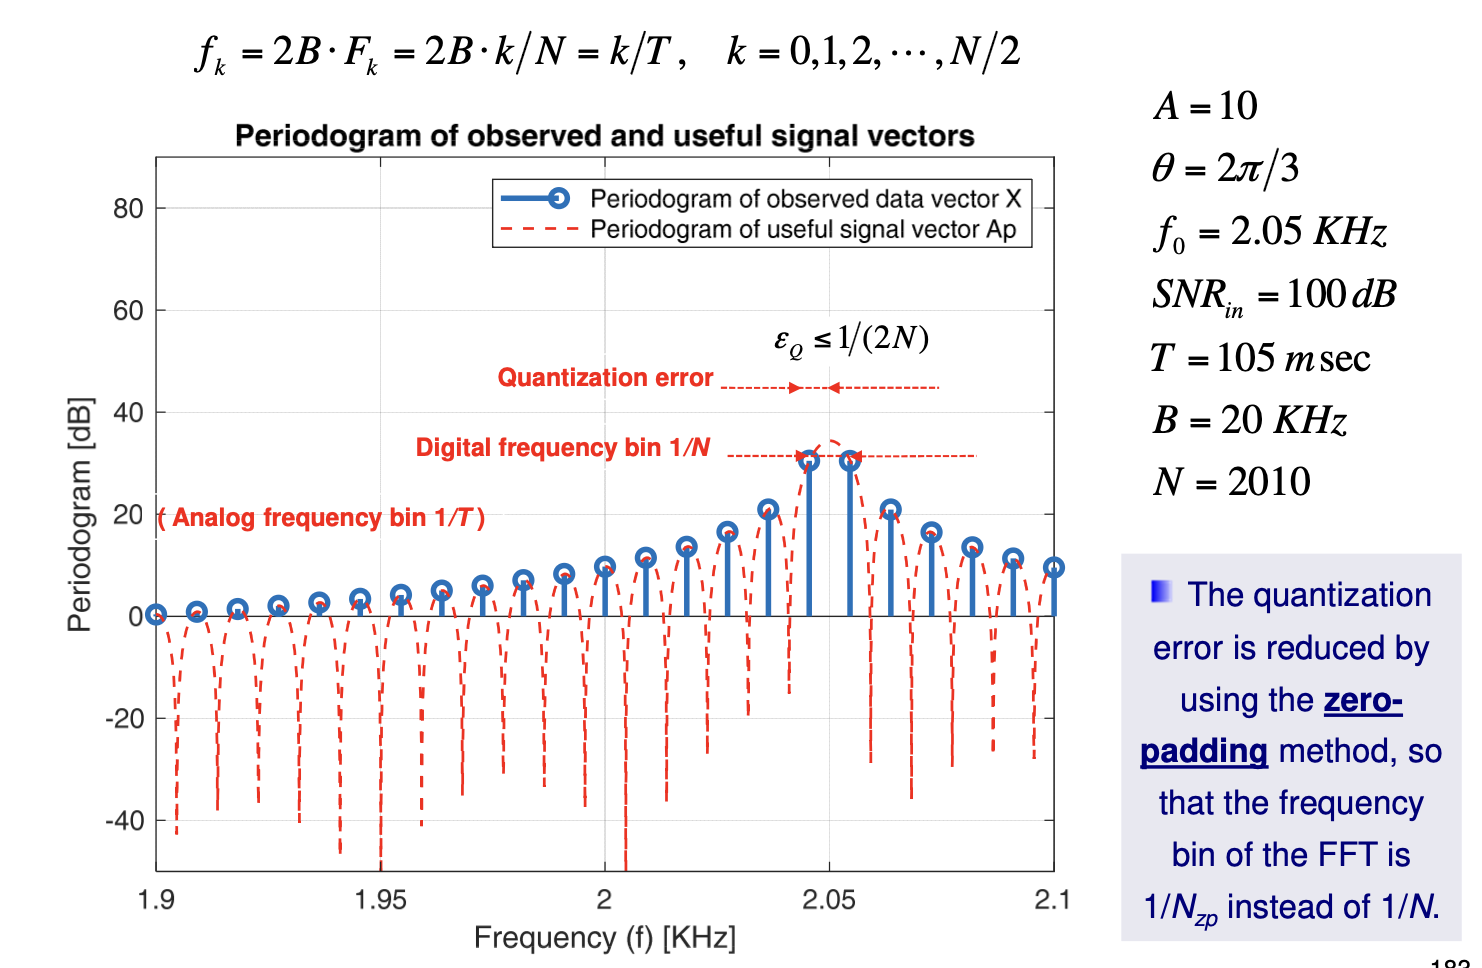
\includegraphics[width=0.65\linewidth]{Image/pdf 4/37.Periodigram.png}
        \label{fig:placeholder}
    \end{figure}
\begin{figure}[H]
    \centering
    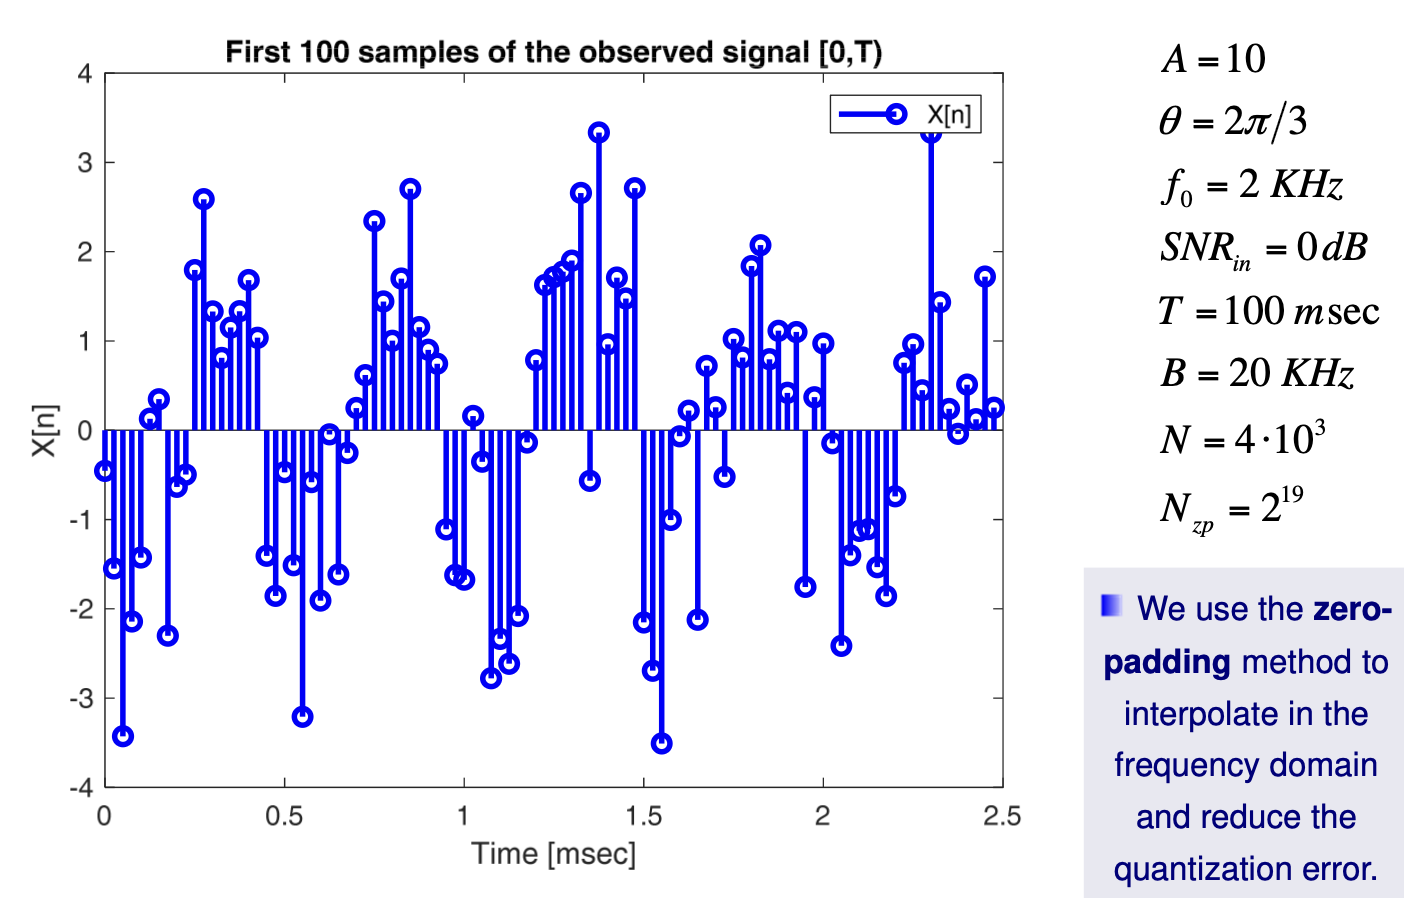
\includegraphics[width=0.65\linewidth]{Image/pdf 4/38.100_values.png}
    \label{fig:placeholder}
\end{figure}
\begin{figure}[H]
    \centering
    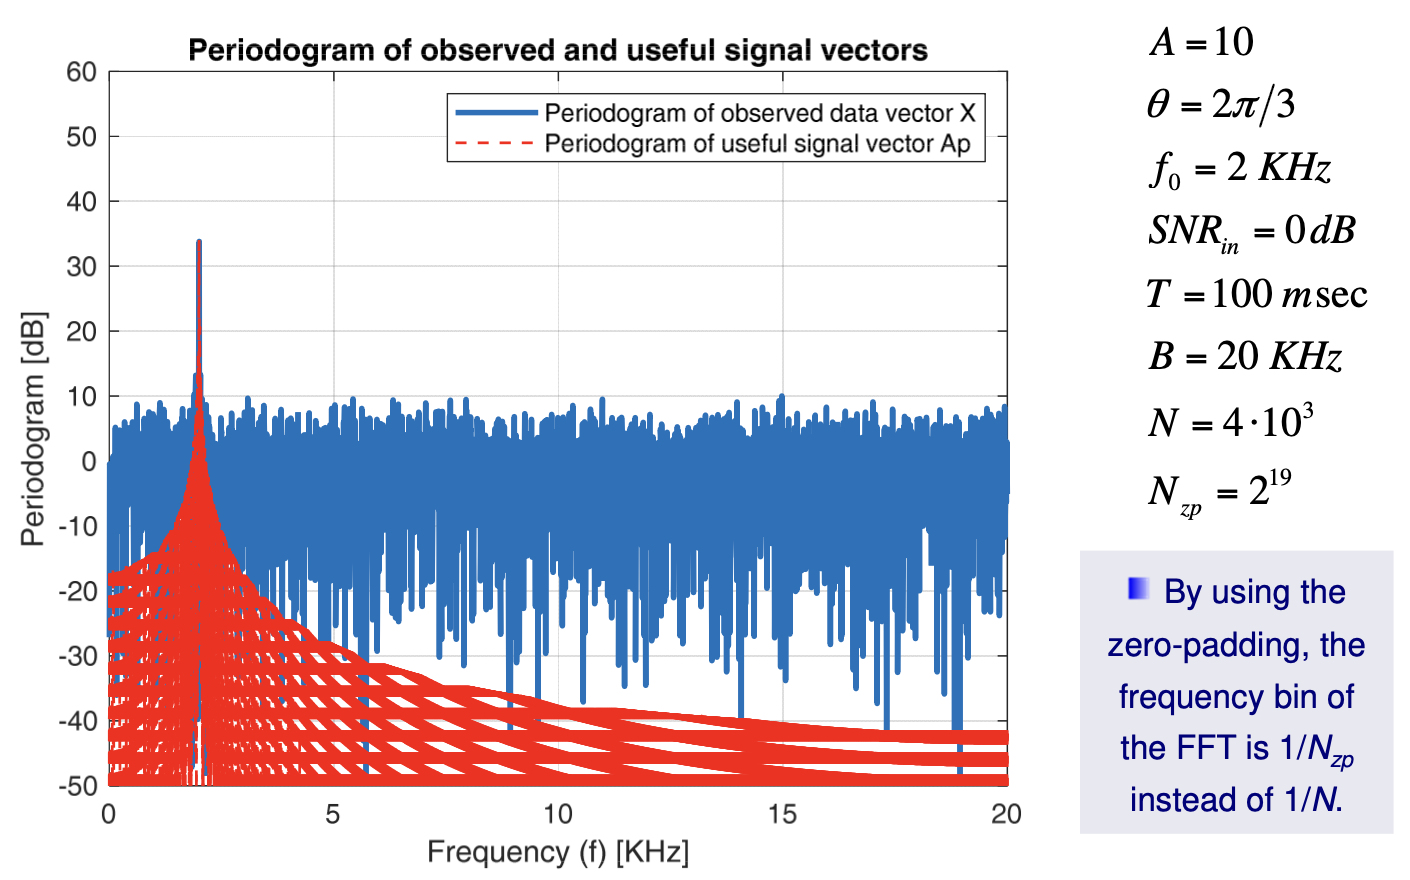
\includegraphics[width=0.65\linewidth]{Image/pdf 4/39.Period_signal_1.png}
    \label{fig:placeholder}
\end{figure}
\begin{figure}[H]
    \centering
    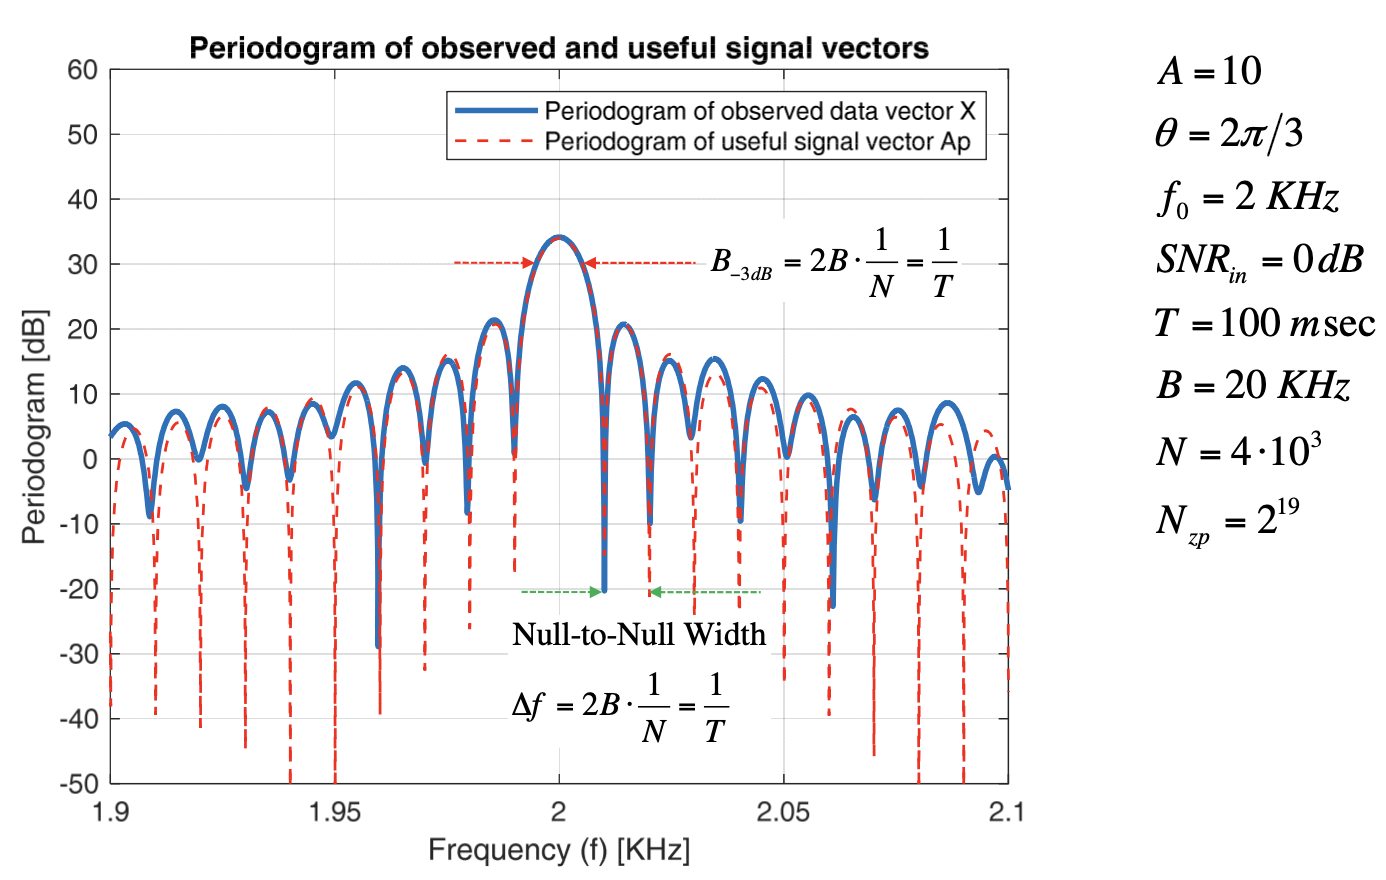
\includegraphics[width=0.65\linewidth]{Image/pdf 4/40.Periodigram_signal_2.png}
    \label{fig:placeholder}
\end{figure}
\begin{figure}[H]
    \centering
    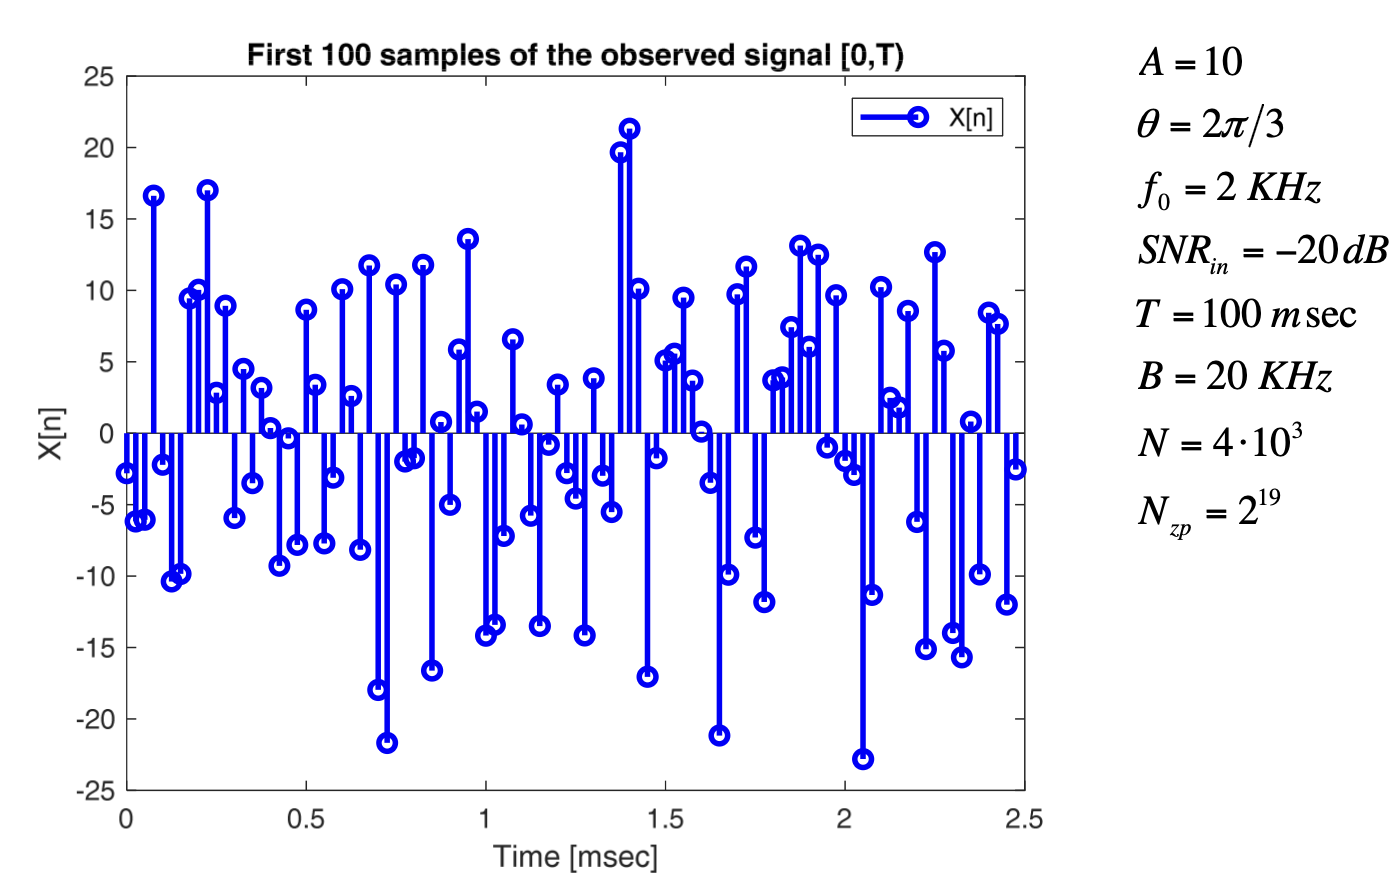
\includegraphics[width=0.65\linewidth]{Image/pdf 4/41.100_values_2.png}
    \label{fig:placeholder}
\end{figure}
\begin{figure}[H]
    \centering
    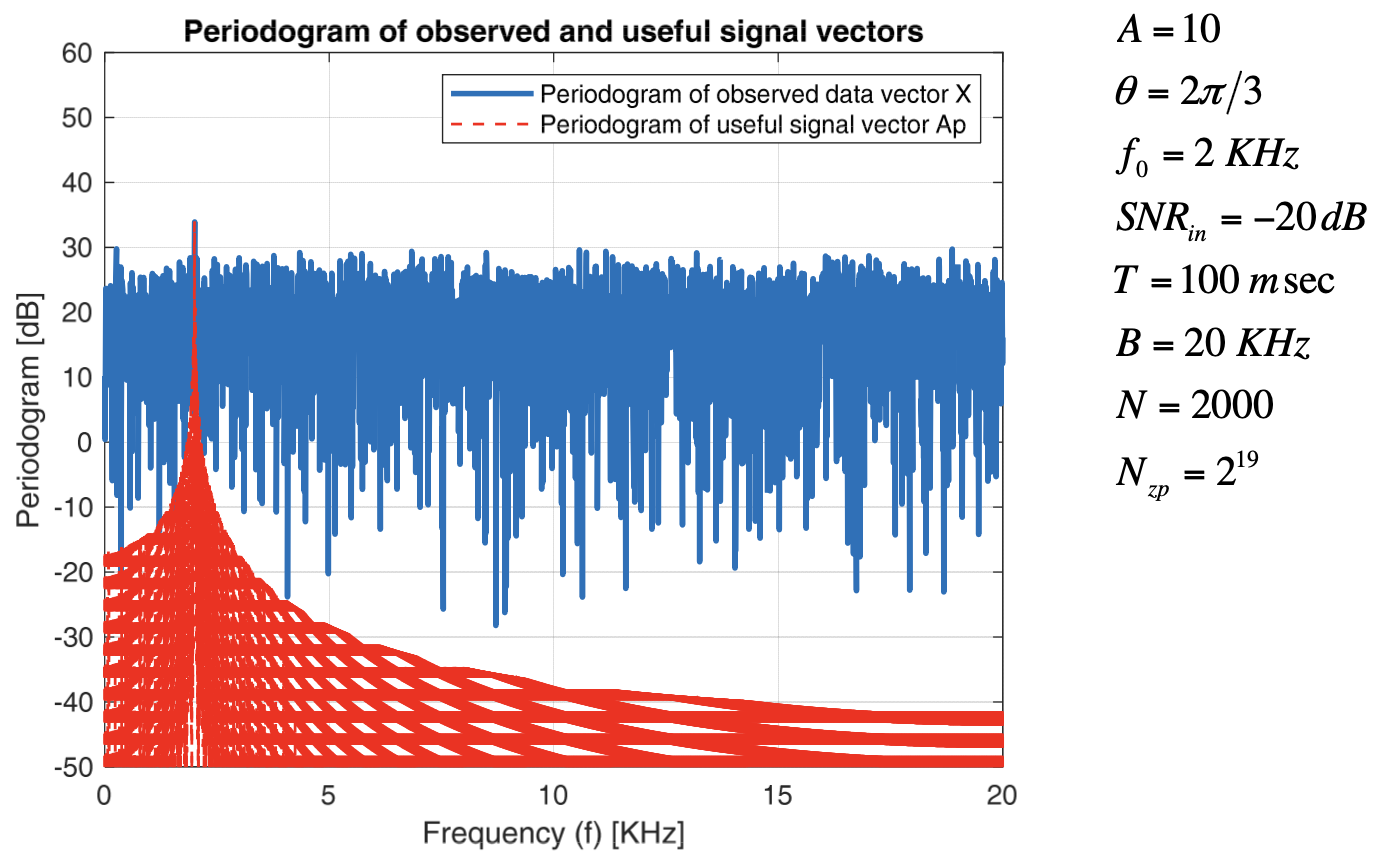
\includegraphics[width=0.65\linewidth]{Image/pdf 4/42.Period_signal_2.png}
    \label{fig:placeholder}
\end{figure}
\begin{figure}[H]
    \centering
    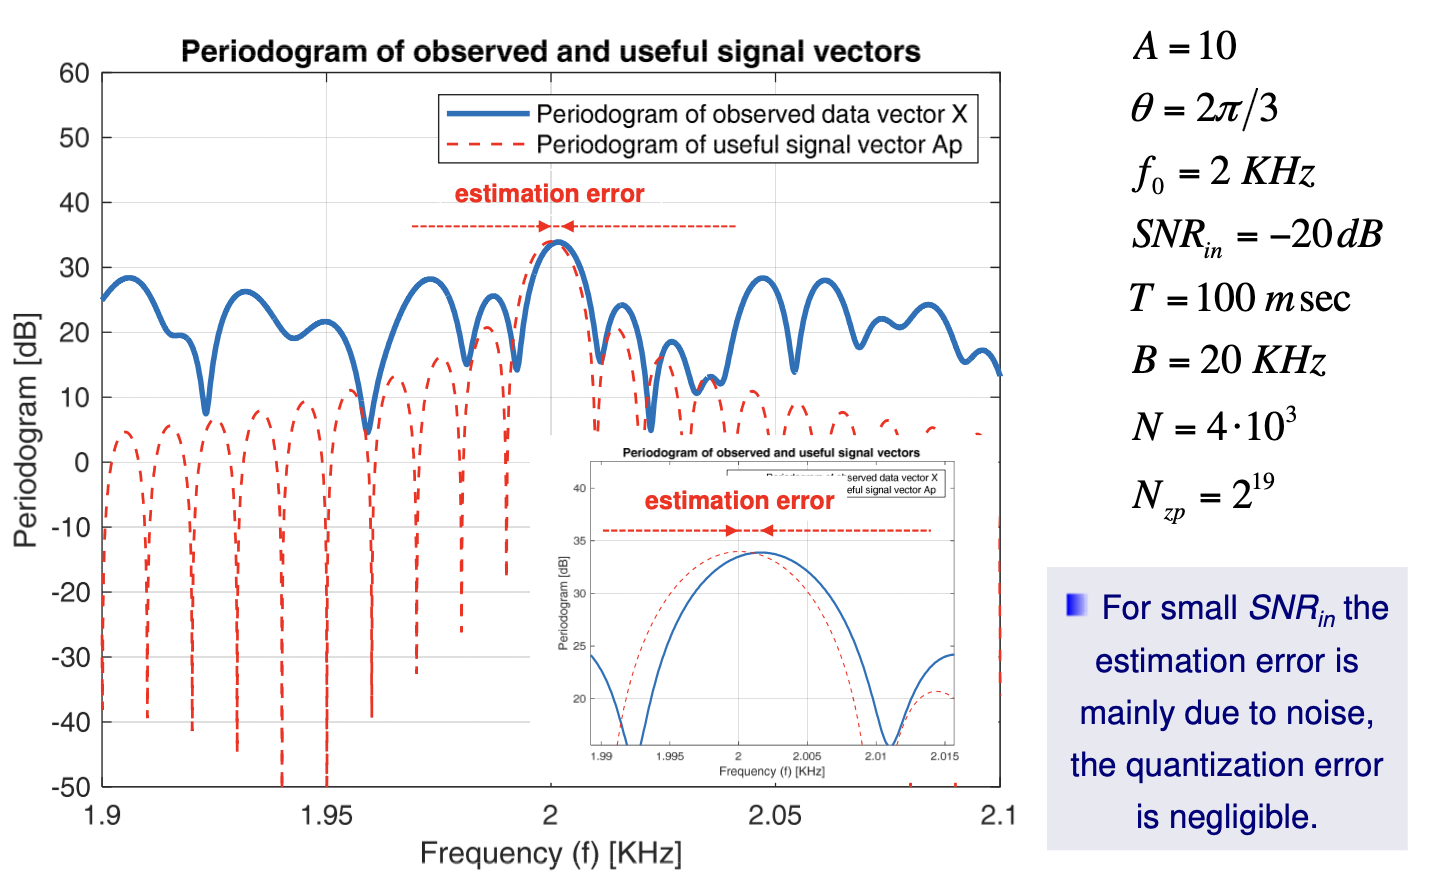
\includegraphics[width=0.65\linewidth]{Image/pdf 4/43.Periodigram_signal_3.png}
    \label{fig:placeholder}
\end{figure}
\begin{figure}[H]
    \centering
    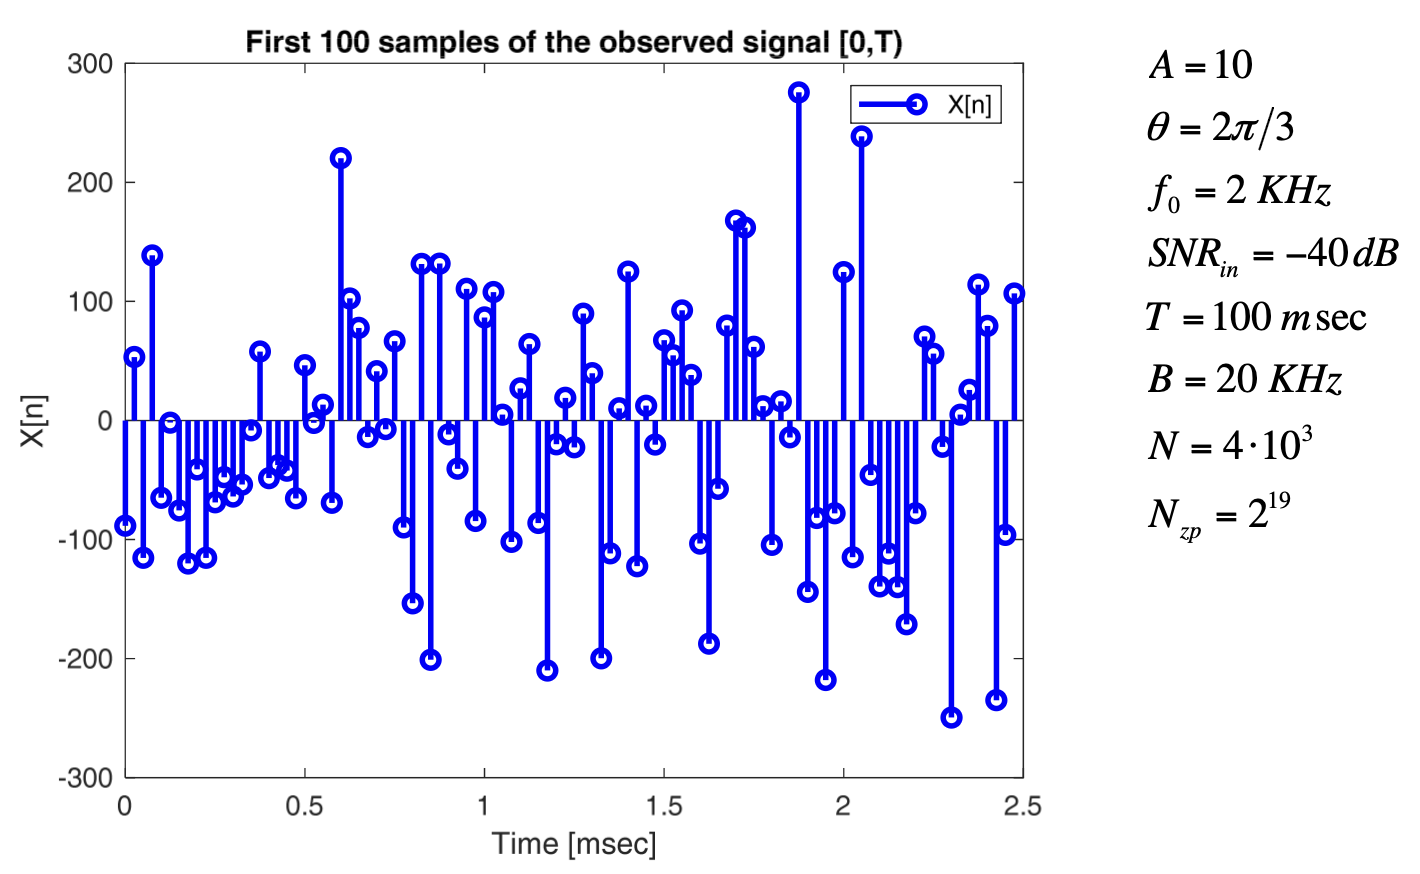
\includegraphics[width=0.65\linewidth]{Image/pdf 4/44.100_values_3.png}
    \label{fig:placeholder}
\end{figure}
\begin{figure}[H]
    \centering
    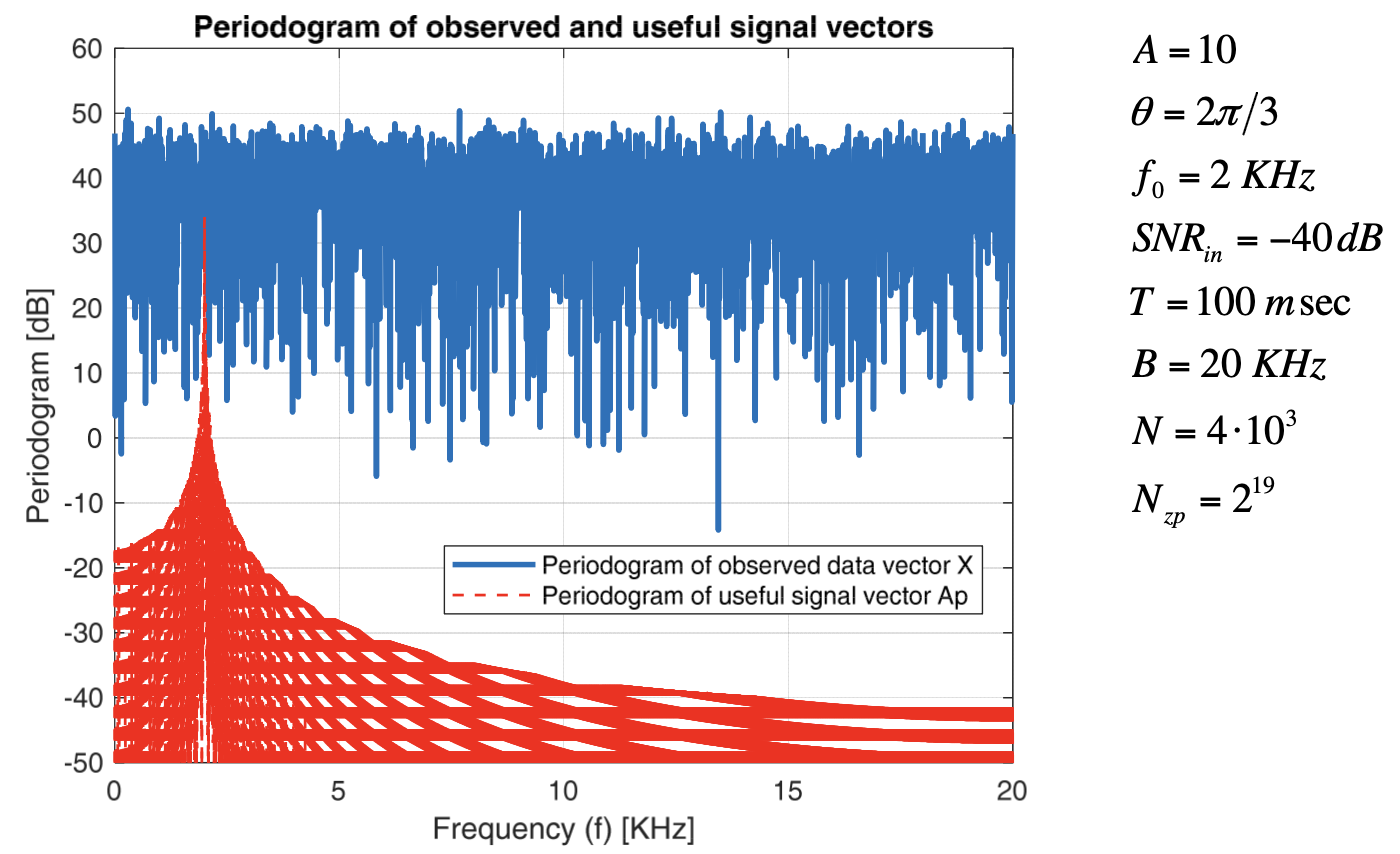
\includegraphics[width=0.65\linewidth]{Image/pdf 4/45.Period_signal_3.png}
    \label{fig:placeholder}
\end{figure}
\begin{figure}[H]
    \centering
    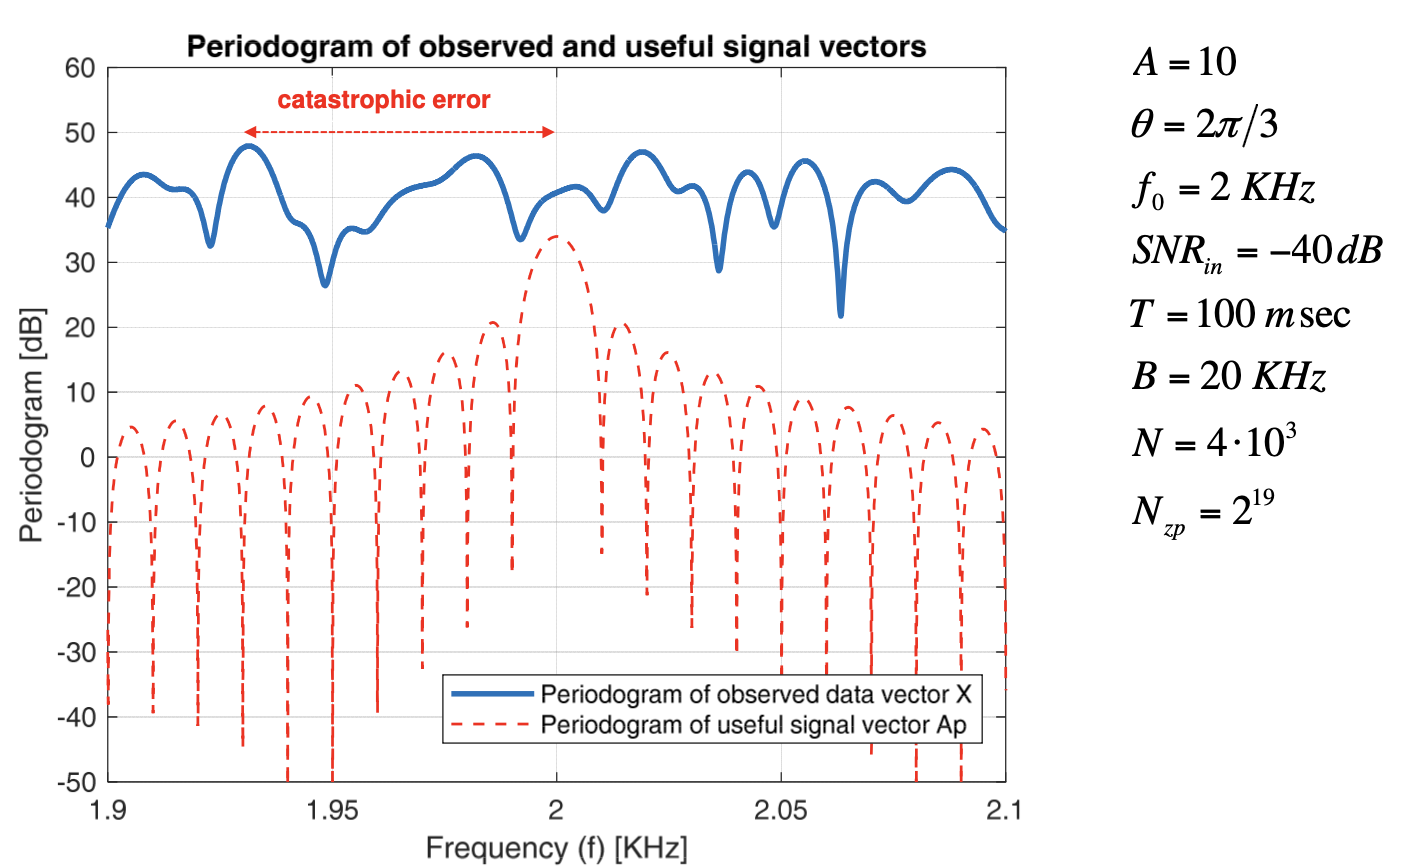
\includegraphics[width=0.65\linewidth]{Image/pdf 4/46.Catastrophic_error.png}
    \label{fig:placeholder}
\end{figure}
\begin{figure}[H]
    \centering
    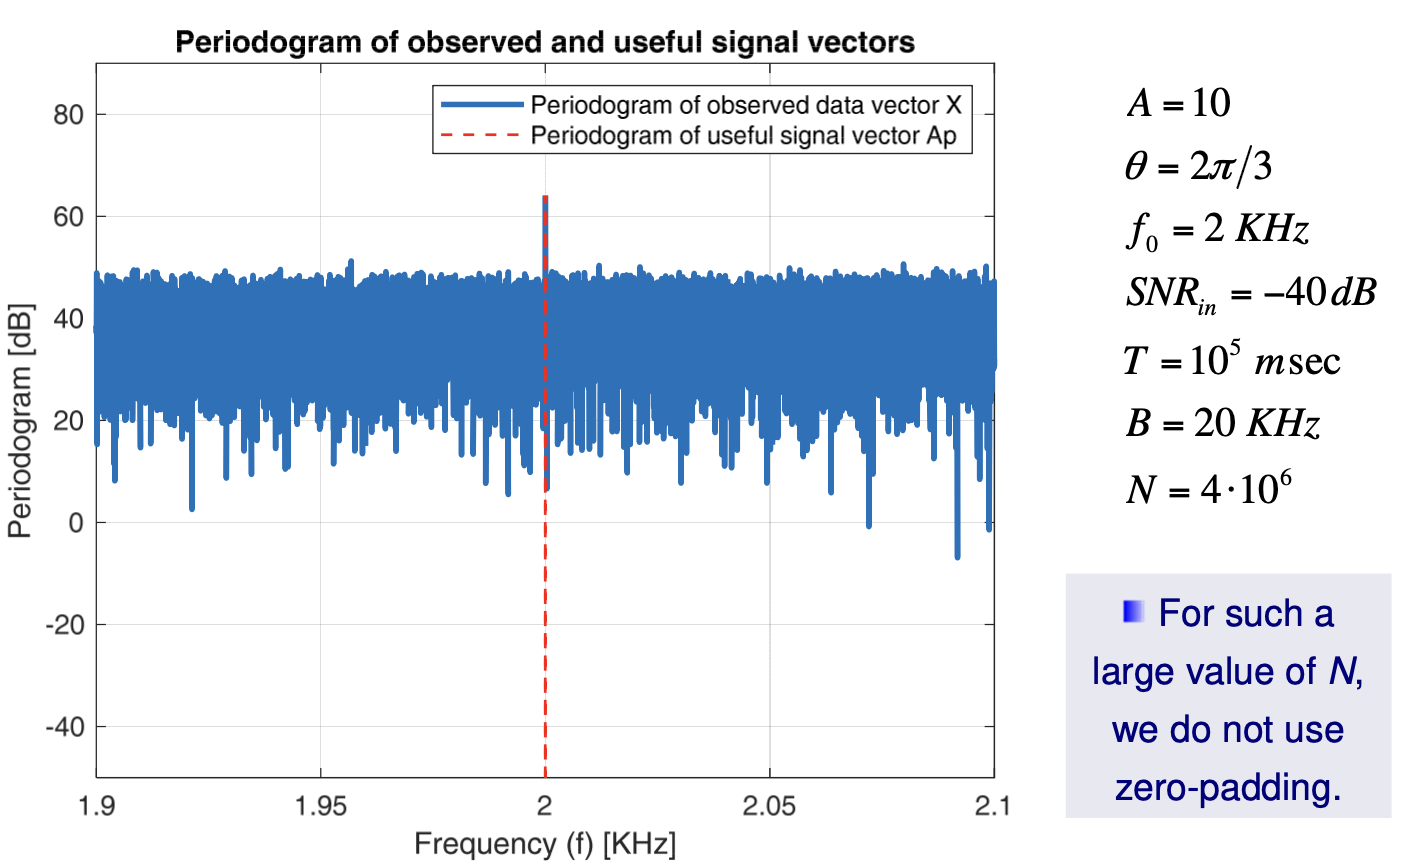
\includegraphics[width=0.65\linewidth]{Image/pdf 4/47.Solution_in_Low_SNR.png}
    \label{fig:placeholder}
\end{figure}
\begin{figure}[H]
    \centering
    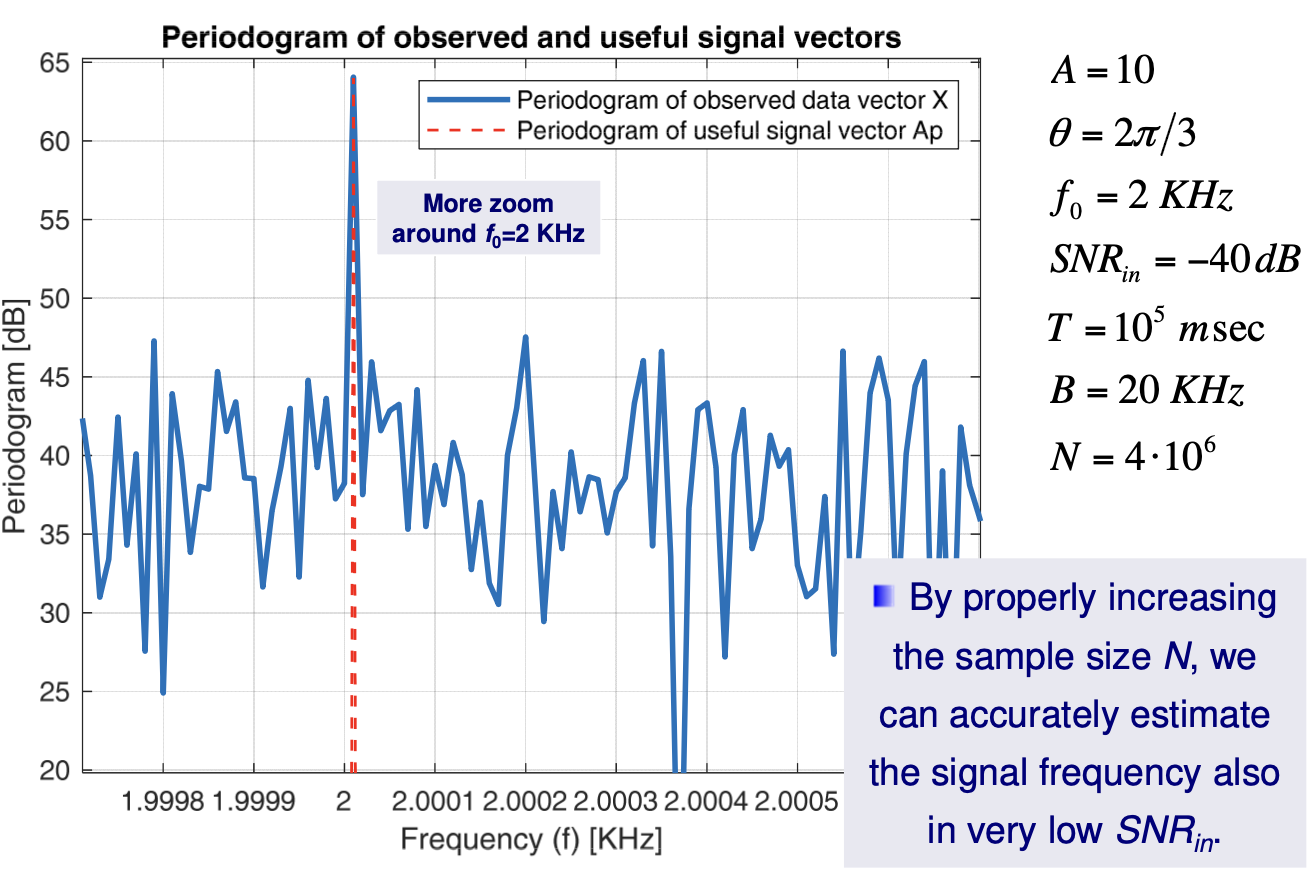
\includegraphics[width=0.65\linewidth]{Image/pdf 4/48.Solution_in_Low_SNR_2.png}
    \label{fig:placeholder}
\end{figure}


    \item \textbf{Cramèr-Rao lower bounds (CRBs)} for the joint estimate of the parameters of a deterministic signal \(s(t;\theta)\) observed in \(t\in[0,T)\) in the presence of AWGN.
    \item After sampling, the data vector is: \(\mathbf{X}=\mathbf{s}(\boldsymbol{\theta})+\mathbf{W}\)
    Where \(\theta\) is the vector of unknown parameters to be estimated.
    \item If the noise \textbf{W} is AWGN:
    \[
    \mathbf{X}\in\mathcal{N}\left(\mathbf{s}(\boldsymbol{\theta}),\frac{N_0}{2}\mathbf{I}\right)
    \]
    \item The log-likehood function (log-LF):
\[
\ln L(\theta) = \ln f_X(\mathbf{x}; \theta) =
- \frac{N}{2} \ln(\pi N_0)
- \frac{1}{N_0} \sum_{i=0}^{N-1} (x_i - s_i(\theta))^2
\]

\[
\text{where} \quad \sum_{i=0}^{N-1} \left(x_i - s_i(\theta)\right)^2 = \left\| \mathbf{x} - \mathbf{s}(\theta) \right\|^2
\]
    \item Let's calculate now the elements of the \textbf{Fisher Information Matrix (FIM)}:
    \[
\left[ \mathbf{I}(\boldsymbol{\theta}) \right]_{i,j}
= -\mathbb{E}\left\{
    \frac{\partial^2 \ln L(\boldsymbol{\theta})}{\partial \theta_i \partial \theta_j}
\right\}, \qquad i,j = 1,2,\ldots,P
\]

\[
\text{where} \quad \boldsymbol{\theta} \triangleq
\begin{bmatrix}
    \theta_1 & \theta_2 & \cdots & \theta_P
\end{bmatrix}^T
\]

\[
\ln L(\boldsymbol{\theta}) = -\frac{N}{2}\ln(\pi N_0)
- \frac{1}{N_0} \sum_{k=0}^{N-1} (x_k - s_k(\boldsymbol{\theta}))^2
\]

\[
\frac{\partial \ln L(\boldsymbol{\theta})}{\partial \theta_i}
= \frac{2}{N_0} \sum_{k=0}^{N-1} \frac{\partial s_k(\boldsymbol{\theta})}{\partial \theta_i}
(x_k - s_k(\boldsymbol{\theta}))
\]

\[
\frac{\partial^2 \ln L(\boldsymbol{\theta})}{\partial \theta_i \partial \theta_j}
= -\frac{2}{N_0}
\sum_{k=0}^{N-1} \frac{\partial s_k(\boldsymbol{\theta})}{\partial \theta_i}
\frac{\partial s_k(\boldsymbol{\theta})}{\partial \theta_j}
+
\frac{2}{N_0}
\sum_{k=0}^{N-1} 
\frac{\partial^2 s_k(\boldsymbol{\theta})}{\partial \theta_i \partial \theta_j}
(x_k - s_k(\boldsymbol{\theta}))
\]
\[
\text{since} \quad x_k \in \mathcal{N}\left(s_k(\boldsymbol{\theta}), \frac{N_0}{2}\right)
\implies
\mathbb{E}\left\{ x_k - s_k(\boldsymbol{\theta}) \right\} = 0
\]
    \item Hence, we get the following general relationship:
\[
\left[ \mathbf{I}(\boldsymbol{\theta}) \right]_{i,j}
= -\mathbb{E}\left\{
    \frac{\partial^2 \ln L(\boldsymbol{\theta})}{\partial \theta_i \partial \theta_j}
\right\}
= \frac{2}{N_0} \sum_{k=0}^{N-1}
    \frac{\partial s_k(\boldsymbol{\theta})}{\partial \theta_i}
    \cdot
    \frac{\partial s_k(\boldsymbol{\theta})}{\partial \theta_j}
\]
    \item We now apply this formula to derive the \textbf{Cramèr-Rao lower bounds (CRBs)} for the joint estimate of amplitude, phase and frequency of a narrowband cosinusoidal signal observed in \(t\in[0,T)\) in the presence of AWGN.
    \item In our case, the vector of unknown parameters to be estimated is:
    \[
    \boldsymbol{\theta}\triangleq[A\quad\theta\quad F_0]^T
    \]
    and the SOI vector is given by:
\[
\mathbf{s}(\boldsymbol{\theta}) = A \cdot \mathbf{p}(\theta, F_0) = \frac{A}{\sqrt{2B}}
\begin{bmatrix}
\cos(\theta) & \cos(2\pi F_0 + \theta) & \cdots & \cos\left(2\pi F_0 (N-1) + \theta\right)
\end{bmatrix}^{T}
\]

\[
s_k(\boldsymbol{\theta}) = \frac{A}{\sqrt{2B}} \cos(2\pi F_0 k + \theta)
\quad \Longrightarrow \quad
\begin{cases}
\frac{\partial s_k(\boldsymbol{\theta})}{\partial A} = \frac{1}{\sqrt{2B}} \cos(2\pi F_0 k + \theta) \\[1em]
\frac{\partial s_k(\boldsymbol{\theta})}{\partial \theta} = -\frac{A}{\sqrt{2B}} \sin(2\pi F_0 k + \theta) \\[1em]
\frac{\partial s_k(\boldsymbol{\theta})}{\partial F_0} = -\frac{2\pi k A}{\sqrt{2B}} \sin(2\pi F_0 k + \theta)
\end{cases}
\]
    \item The FIM elements are:
    \[
\mathbf{s}(\boldsymbol{\theta}) = A \cdot \mathbf{p}(\theta, F_0) = \frac{A}{\sqrt{2B}}
\begin{bmatrix}
\cos(\theta) & \cos(2\pi F_0 + \theta) & \cdots & \cos\left(2\pi F_0 (N-1) + \theta\right)
\end{bmatrix}^{T}
\]

\[
s_k(\boldsymbol{\theta}) = \frac{A}{\sqrt{2B}} \cos(2\pi F_0 k + \theta)
\quad \Longrightarrow \quad
\begin{cases}
\frac{\partial s_k(\boldsymbol{\theta})}{\partial A} = \frac{1}{\sqrt{2B}} \cos(2\pi F_0 k + \theta) \\[1em]
\frac{\partial s_k(\boldsymbol{\theta})}{\partial \theta} = -\frac{A}{\sqrt{2B}} \sin(2\pi F_0 k + \theta) \\[1em]
\frac{\partial s_k(\boldsymbol{\theta})}{\partial F_0} = -\frac{2\pi k A}{\sqrt{2B}} \sin(2\pi F_0 k + \theta)
\end{cases}
\]
    \item Where:
    \[
    SNR_{in}=\frac{A^2}{2N_0B}=\frac{A^2T}{N_0N}
    \]
    \item Other component:
\begin{align*}
\left[\mathbf{I}(\boldsymbol{\theta})\right]_{3,3}
&= \frac{2}{N_0} \sum_{k=0}^{N-1}
\left[
    -\frac{2\pi k A}{\sqrt{2B}} \sin(2\pi F_0 k + \theta)
\right]^2
= \frac{2}{N_0} \cdot \frac{4\pi^2 A^2}{2B} \sum_{k=0}^{N-1} k^2 \sin^2(2\pi F_0 k + \theta)\\
&= \frac{4\pi^2 A^2}{N_0 B} \sum_{k=0}^{N-1} k^2 \left[ \frac{1}{2} - \frac{1}{2} \cos(4\pi F_0 k + 2\theta) \right]\\
&= \frac{2\pi^2 A^2}{N_0 B} \sum_{k=0}^{N-1} k^2
- \frac{2\pi^2 A^2}{N_0 B} \sum_{k=0}^{N-1} k^2 \cos(4\pi F_0 k + 2\theta)\\
&\simeq \frac{2\pi^2 A^2}{N_0 B} \sum_{k=0}^{N-1} k^2
= \frac{2\pi^2 A^2}{N_0 B} \cdot \frac{N(N-1)(2N-1)}{6}\\
&= \frac{2\pi^2 A^2 T}{3 N_0} (N-1)(2N-1)
\end{align*}


    \item Where we used the fact that for \(N\gg 1\):
    \[
    \frac{1}{N}\sum_{k=0}^{N-1}k^2\cos(4\pi F_0k+2\theta)\approx0
    \]
\item Other components:
\begin{align*}
\left[\mathbf{I}(\boldsymbol{\theta})\right]_{1,2}
&= \left[\mathbf{I}(\boldsymbol{\theta})\right]_{2,1}
= \frac{2}{N_0} \sum_{k=0}^{N-1} \left[
    \frac{1}{\sqrt{2B}} \cos(2\pi F_0 k + \theta)
\right] \left[
    -\frac{A}{\sqrt{2B}} \sin(2\pi F_0 k + \theta)
\right]\\
&= -\frac{A}{N_0 B} \sum_{k=0}^{N-1} \cos(2\pi F_0 k + \theta) \sin(2\pi F_0 k + \theta)\\
&= -\frac{A}{2N_0 B} \sum_{k=0}^{N-1} [\sin(4\pi F_0 k + 2\theta) + \sin(0)]\\
&= -\frac{A N}{2N_0 B} \cdot \frac{1}{N} \sum_{k=0}^{N-1} \sin(4\pi F_0 k + 2\theta) \simeq 0
\end{align*}
    \item Where we the fact that for \(N\gg 1\):
    \[
    \frac{1}{N}\sum_{k=0}^{N-1}\sin(4\pi F_0k+2\theta)\approx0
    \]
    \item Other component:
    \begin{align*}
[I(\theta)]_{1,3} &= [I(\theta)]_{3,1} \\
&= \frac{2}{N_0} \sum_{k=0}^{N-1}
   \left[ \frac{1}{\sqrt{2B}} \cos(2\pi F_0 k + \theta) \right]
   \left[ -\frac{2\pi k A}{\sqrt{2B}} \sin(2\pi F_0 k + \theta) \right] \\
&= -\frac{2\pi A}{N_0 B} \sum_{k=0}^{N-1}
   k \cos(2\pi F_0 k + \theta) \sin(2\pi F_0 k + \theta) \\
&= -\frac{2\pi A}{2 N_0 B} \sum_{k=0}^{N-1}
   k \left[ \sin(4\pi F_0 k + 2\theta) + \sin(0) \right] \\
&= -\frac{\pi A N}{N_0 B} \cdot \frac{1}{N} \sum_{k=0}^{N-1}
   k \sin(4\pi F_0 k + 2\theta) \cong 0
\end{align*}
    \item Where we used the fact that for \(N\gg1\):
    \[
    \frac{1}{N}\sum_{k=0}^{N-1}k\sin(4\pi F_0k+2\theta)\simeq0
    \]
    \item Other components:
    \begin{align*}
[I(\theta)]_{2,3} &= [I(\theta)]_{3,2} \\
&= \frac{2}{N_0} \sum_{k=0}^{N-1}
   \left[ -\frac{A}{\sqrt{2B}} \sin(2\pi F_0 k + \theta) \right]
   \left[ -\frac{2\pi k A}{\sqrt{2B}} \sin(2\pi F_0 k + \theta) \right] \\
&= \frac{2\pi A^2}{N_0 B} \sum_{k=0}^{N-1}
   k \sin^{2}(2\pi F_0 k + \theta) \\
&= \frac{2\pi A^2}{2 N_0 B} \sum_{k=0}^{N-1}
   k \left[ 1 - \cos(4\pi F_0 k + 2\theta) \right] \\
&= \frac{\pi A^2}{N_0 B} \sum_{k=0}^{N-1} k
   - \frac{\pi A N}{N_0 B} \cdot \frac{1}{N}
     \sum_{k=0}^{N-1} k \cos(4\pi F_0 k + 2\theta) \\
&\cong \frac{\pi A^2}{N_0 B} \sum_{k=0}^{N-1} k
   = \frac{\pi A^2}{N_0 B} \cdot \frac{N(N-1)}{2}
   = \frac{\pi A^2 T (N-1)}{N_0}
\end{align*}
    \item Where we used the fact that for \(N\gg 1\):
    \[
    \frac{1}{N}\sum_{k=0}^{N-1}k\cos(4\pi F_0 k+2\theta)\simeq0
    \]

    \item The FIM is finally obtained:
    \begin{align*}
I(\theta)
&=
\begin{bmatrix}
\dfrac{T}{N_0} & 0 & 0 \\[8pt]
0 & \dfrac{A^{2}T}{N_0} & \dfrac{\pi A^{2}T (N-1)}{N_0} \\[8pt]
0 & \dfrac{\pi A^{2}T (N-1)}{N_0} &
   \dfrac{2\pi^{2}A^{2}T (N-1)(2N-1)}{3N_0}
\end{bmatrix} \\[8pt]
&=
\dfrac{A^{2}T}{N_0}
\begin{bmatrix}
\dfrac{1}{A^{2}} & 0 & 0 \\[8pt]
0 & 1 & \pi (N-1) \\[8pt]
0 & \pi (N-1) & \dfrac{2\pi^{2}(N-1)(2N-1)}{3}
\end{bmatrix}
\end{align*}
    \item The inverse of the FIM:     
    \begin{align*}
\operatorname{CRB}(\boldsymbol{\theta})
&= \boldsymbol{I}^{-1}(\boldsymbol{\theta})
   = \frac{N_0}{A^{2} T}
\begin{bmatrix}
\dfrac{1}{A^{2}} & 0 & 0 \\[4pt]
0 & 1 & \pi (N-1) \\[4pt]
0 & \pi (N-1) & \dfrac{2\pi^{2} (N-1)(2N-1)}{3}
\end{bmatrix}^{-1} \\[6pt]
&= \frac{N_0}{A^{2} T}
\begin{bmatrix}
A^{2} & 0 & 0 \\[4pt]
0 & \dfrac{2(2N-1)}{N+1} & -\dfrac{3}{\pi (N+1)} \\[4pt]
0 & -\dfrac{3}{\pi (N+1)} & \dfrac{3}{\pi^{2} (N^{2}-1)}
\end{bmatrix}
\end{align*}
    \item We note that the estimate of the amplitude is decoupled from the estimate of phase and frequency. This is true asymptotically (large \(N\)), sice the ML estimators are asymptotically efficient, but not always efficient.
    \item The CRB's on the three parameters are given by:
    \[
    SNR_{in}=\frac{A^2}{2N_0B}
    \]
    \begin{align*}
\operatorname{CRB}(A)
&= \bigl[ I^{-1}(\theta) \bigr]_{1,1}
   = \frac{N_0}{T}
   = \frac{A^{2}}{N \cdot \mathrm{SNR}_{\mathrm{in}}} \\[6pt]
\operatorname{CRB}(\theta)
&= \bigl[ I^{-1}(\theta) \bigr]_{2,2}
   = \frac{N_0}{A^{2} T} \cdot \frac{2(2N-1)}{N+1}
   = \frac{2(2N-1)}{N (N+1) \mathrm{SNR}_{\mathrm{in}}} \\[6pt]
\operatorname{CRB}(F_0)
&= \bigl[ I^{-1}(\theta) \bigr]_{3,3}
   = \frac{N_0}{A^{2} T} \cdot \frac{3}{\pi^{2} (N^{2}-1)}
   = \frac{3}{\pi^{2} N (N^{2}-1) \mathrm{SNR}_{\mathrm{in}}}
\end{align*}
    \item The CRB's on the analog frequency \(f_0=F_0/T_c=(2B)F_0\) is easily obtained:
\[
\operatorname{CRB}(f_{0})= (2B)^{2} \cdot \operatorname{CRB}(F_{0}) = \frac{N_{0}}{A^{2} T} \cdot \frac{12 B^{2}}{\pi^{2} (N^{2}-1)} = \frac{12 B^{2}}{\pi^{2} N (N^{2}-1)\,\mathrm{SNR}_{\mathrm{in}}}
\]
    \begin{figure}[H]
        \centering
        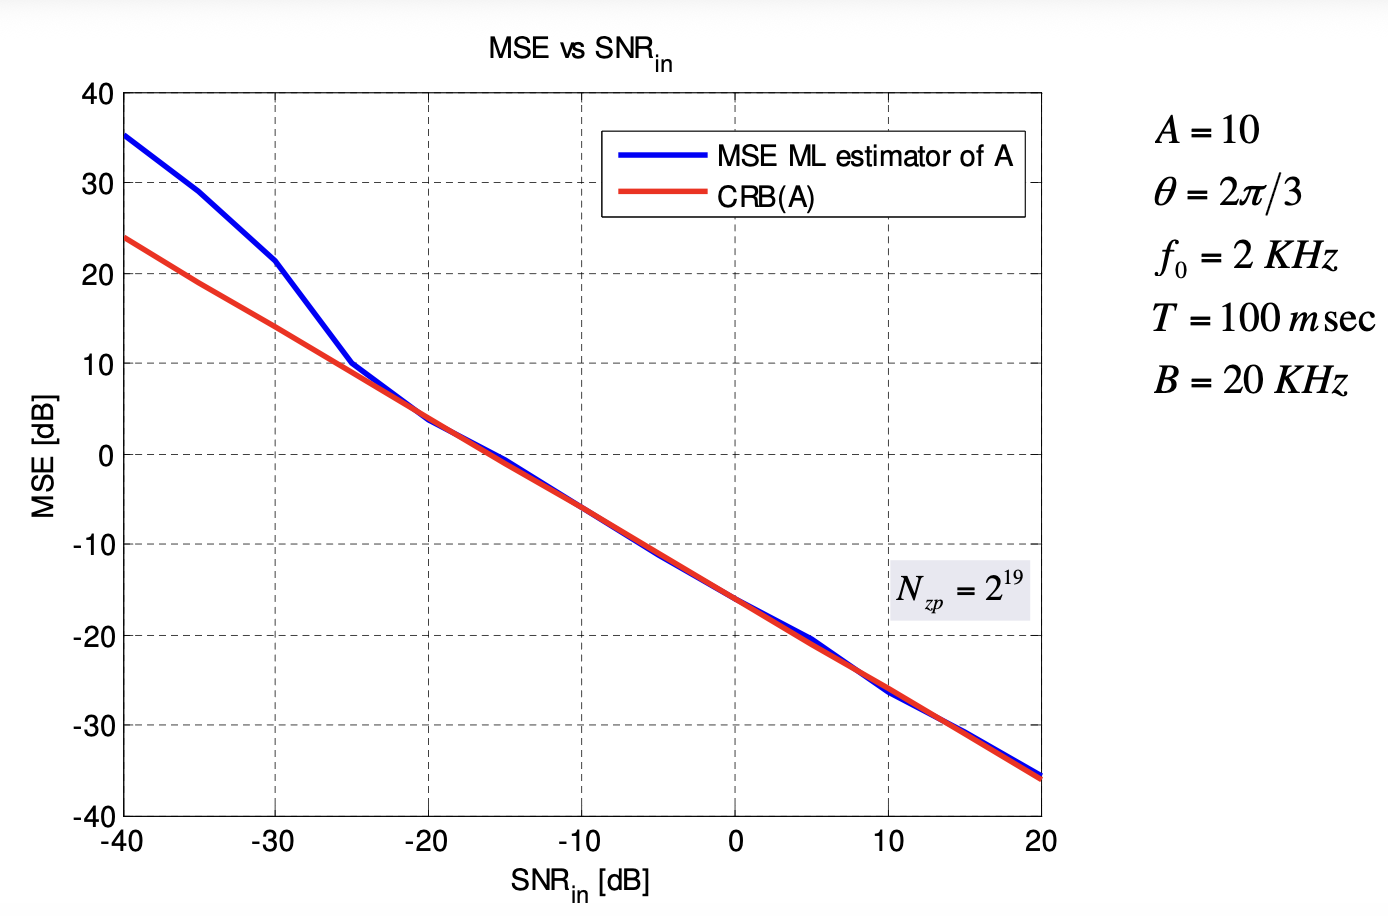
\includegraphics[width=0.6\linewidth]{Image/pdf 4/49.MSE_vs_SNR.png}
        \label{fig:placeholder}
    \end{figure}
    \begin{figure}[H]
        \centering
        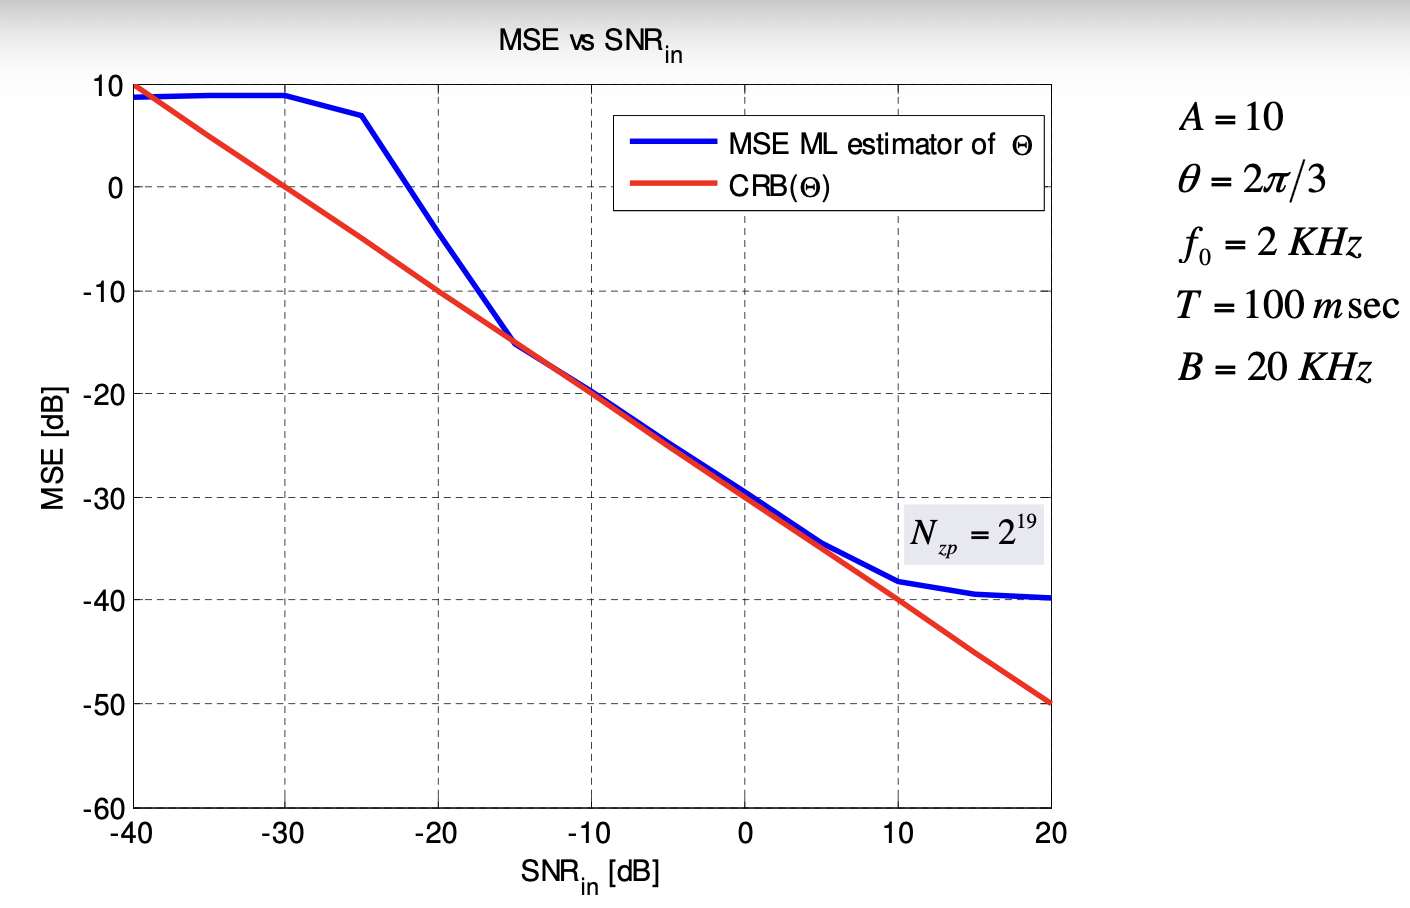
\includegraphics[width=0.6\linewidth]{Image/pdf 4/50.MSE_vs_SNR_2.png}
        \label{fig:placeholder}
    \end{figure}
    \begin{figure}[H]
        \centering
        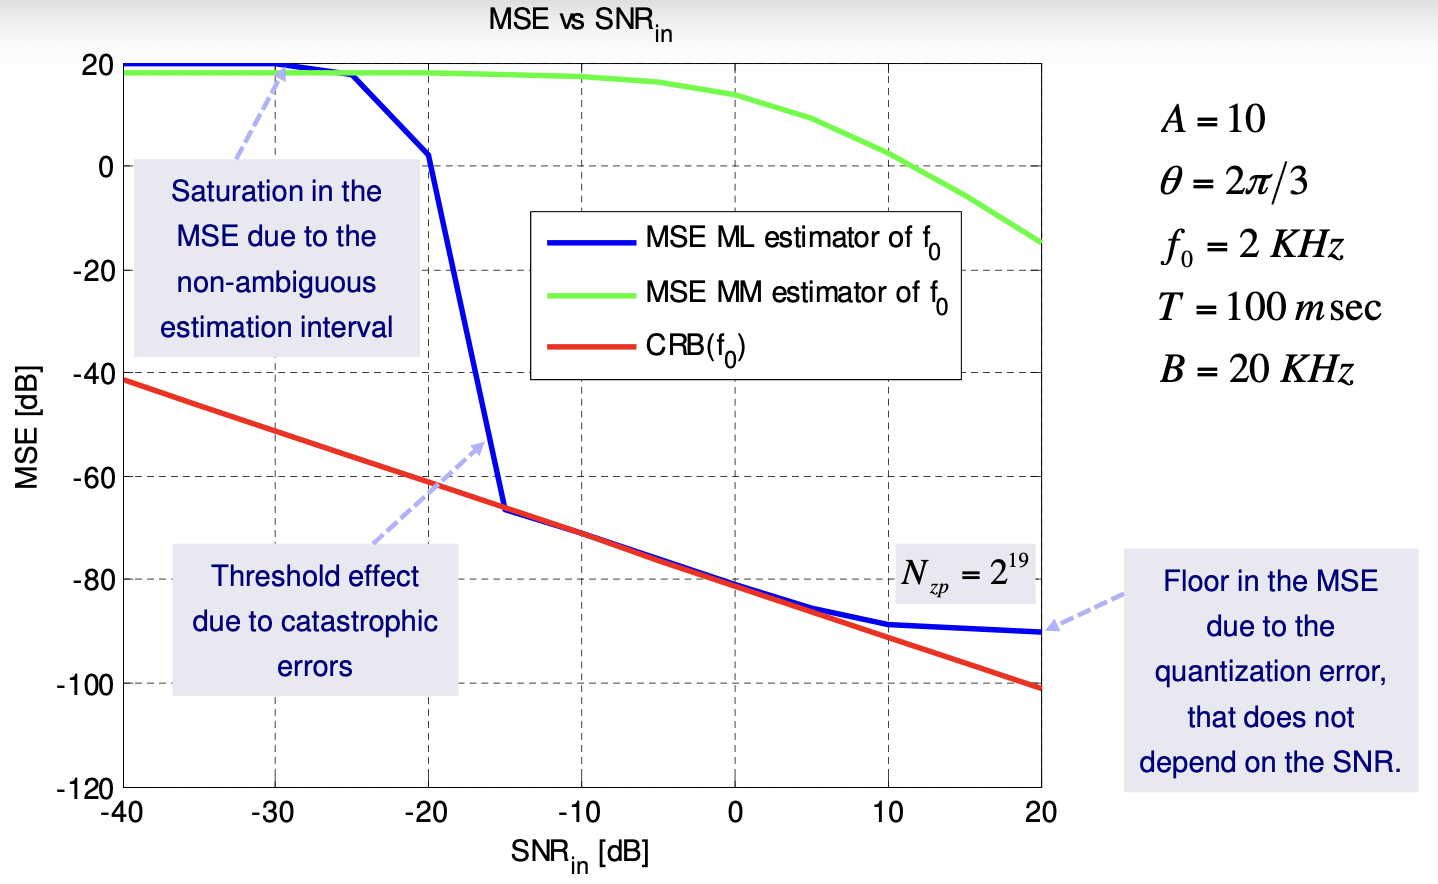
\includegraphics[width=0.6\linewidth]{Image/pdf 4/51.MSE_vs_SNR_3.png}
        \label{fig:placeholder}
    \end{figure}
    \begin{figure}[H]
        \centering
        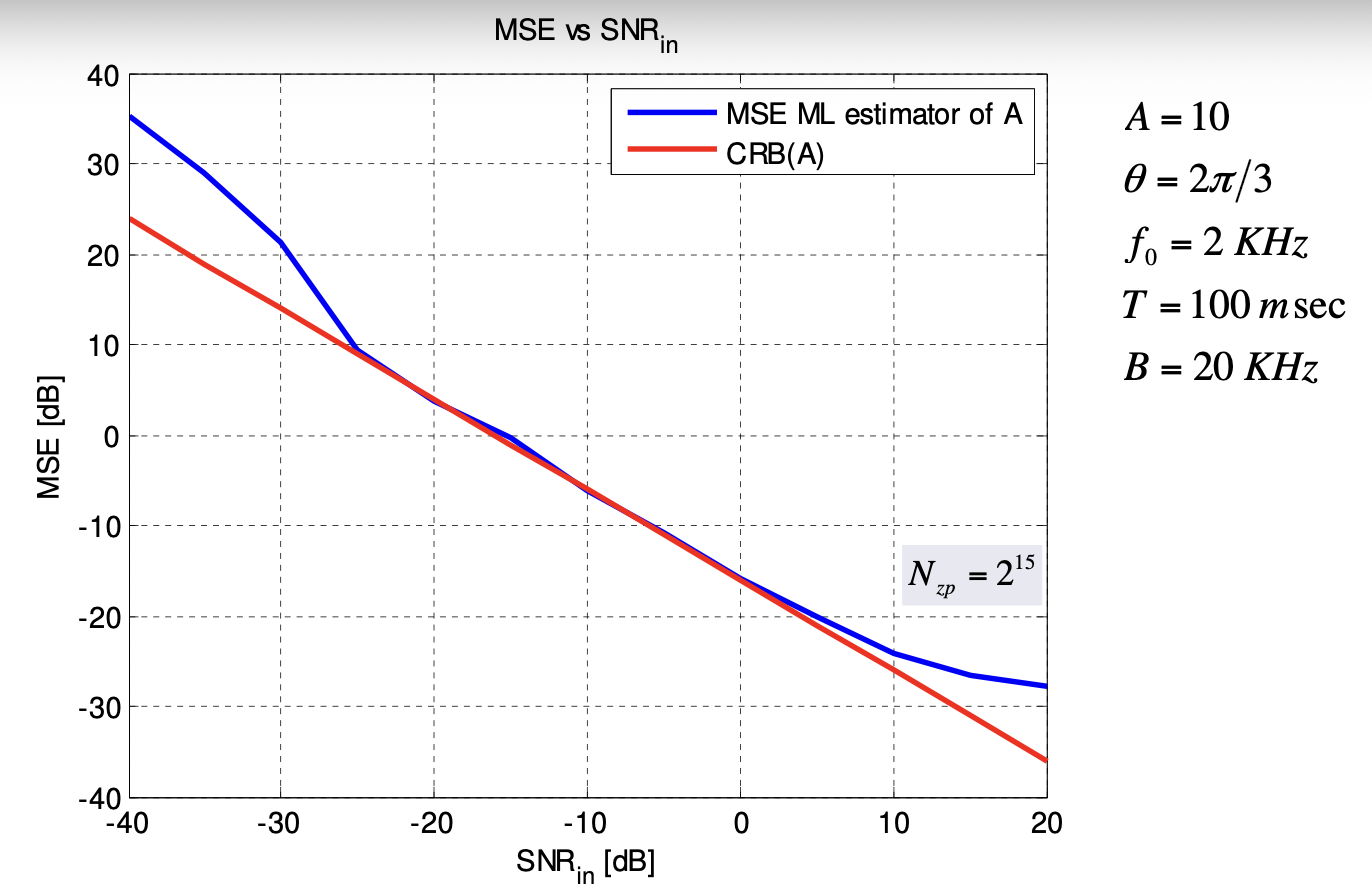
\includegraphics[width=0.6\linewidth]{Image/pdf 4/52.MSE_vs_SNR_4.png}
        \label{fig:placeholder}
    \end{figure}
    \begin{figure}[H]
        \centering
        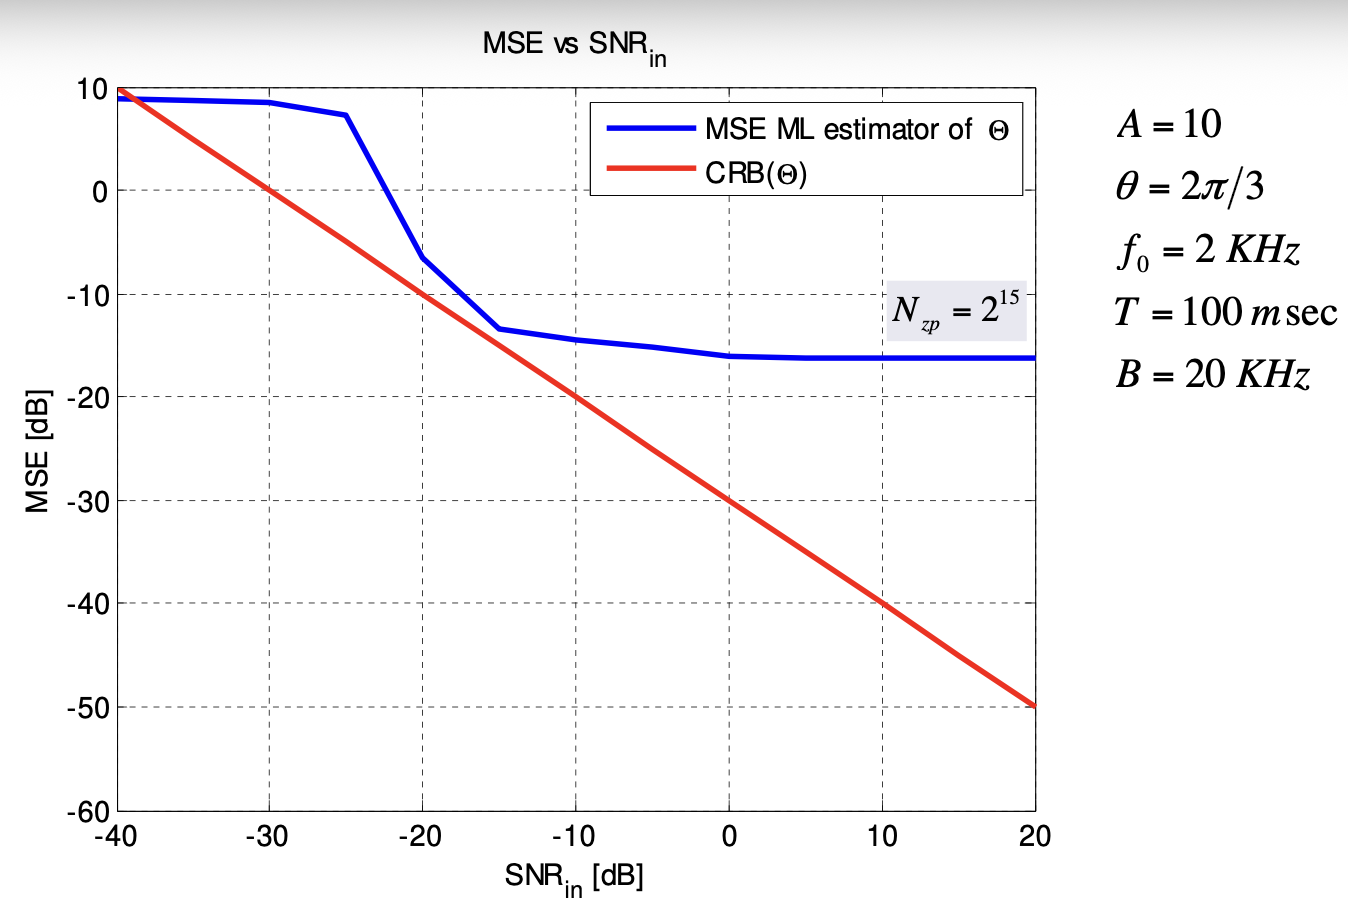
\includegraphics[width=0.6\linewidth]{Image/pdf 4/53.MSE_vs_SNR_5.png}
        \label{fig:placeholder}
    \end{figure}
    \begin{figure}[H]
        \centering
        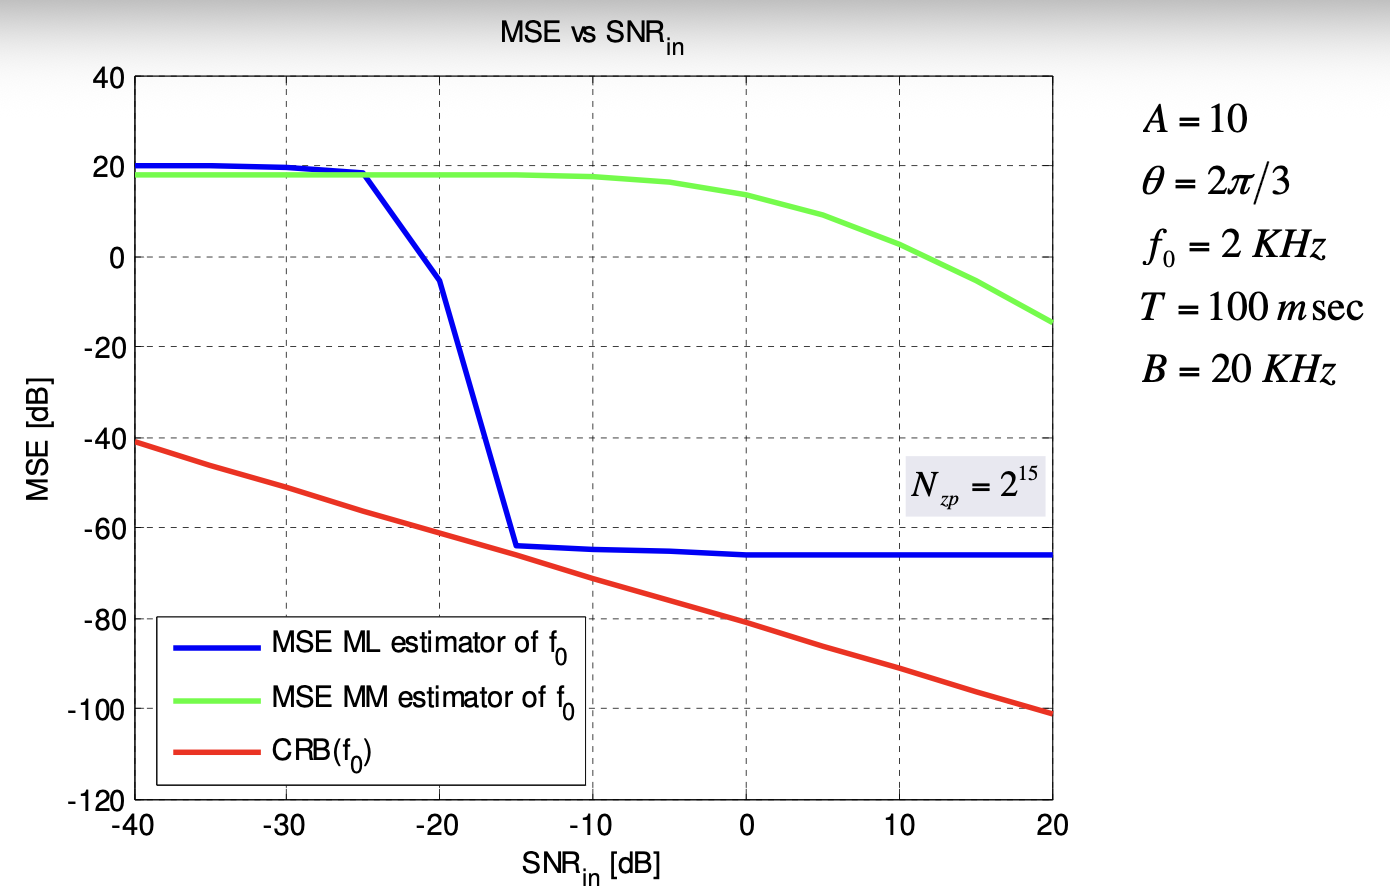
\includegraphics[width=0.6\linewidth]{Image/pdf 4/54.MSE_vs_SNR_6.png}
        \label{fig:placeholder}
    \end{figure}
    \item The ML estimator frequency \(f_0\) has high computational complexity, since it require calculation of FFT of high order and then a search for the location of the maximum.
    \item An alternative estimator can be derived by the \textbf{Method of Moments (MM)}.
    \item To calculate the moments of the observed data, let us assume that the initial phase \(\theta\) is uniformly distributed in \([+\pi,-\pi)\).
    \item The mean value does not contain any information on \(f_0\):
    \begin{align*}
\eta_X[k] &\triangleq E\{X_k\}
= E\left\{ \frac{1}{\sqrt{2B}}\, X_B\!\left( \frac{k}{2B} \right) \right\} \\[4pt]
&= \frac{A}{\sqrt{2B}}\, E\{\cos(2\pi F_0 k + \theta)\}
   + \frac{1}{\sqrt{2B}}\, E\left\{ W_B\!\left( \frac{k}{2B} \right) \right\} \\[4pt]
&= \frac{A}{\sqrt{2B}}\, \frac{1}{2\pi}
   \int_{-\pi}^{\pi} \cos(2\pi F_0 k + \theta)\, d\theta
   + \frac{1}{\sqrt{2B}}\, E\left\{ W_B\!\left( \frac{k}{2B} \right) \right\}
   = 0
\end{align*}
    \item Let us calculate the observed data Autocorrelation Function (ACF):
    \begin{align*}
R_X[k,k+m]
&\triangleq E\{X_k X_{k+m}\}
= \frac{1}{2B}\,
  E\left\{ X_B\!\left(\frac{k}{2B}\right)
           X_B\!\left(\frac{k+m}{2B}\right) \right\} \\[4pt]
&= \frac{A^{2}}{2B} \cdot \frac{1}{2\pi}
   \int_{-\pi}^{\pi}
     \cos(2\pi F_{0}k + \theta)\,
     \cos\!\bigl(2\pi F_{0}(k+m) + \theta\bigr)\, d\theta \\[4pt]
&\quad
 + \frac{1}{2B}\,
   E\left\{ W_B\!\left(\frac{k}{2B}\right)
            W_B\!\left(\frac{k+m}{2B}\right) \right\} \\[4pt]
&= \frac{A^{2}}{2B} \cdot \frac{1}{2} \cos(2\pi F_{0} m)
   + \frac{1}{2B}\, R_{W_B}\!\left(\frac{m}{2B}\right) \\[4pt]
&= \frac{A^{2}}{4B} \cos(2\pi F_{0} m)
   + \frac{1}{2B}\, N_{0} B\,
     \operatorname{sinc}\left(2B \frac{m}{2B}\right) \\[4pt]
&= \frac{A^{2}}{4B} \cos(2\pi F_{0} m)
   + \frac{N_{0}}{2}\, \delta[m] .
\end{align*}
    \item The ACF provides the information we are looking for:
    \[
    R_X[m]=\frac{A^2}{4B}\cos(2\pi F_0m)+\frac{N_0}{2}\cdot\delta[m]
    \]
    \item In fact, if we calculate the ACF for lag 0 and 1 we get:
    \[
R_X[0]
= \frac{A^{2}}{4B} + \frac{N_0}{2}
= \frac{A^{2}}{4B}\left(1 + \frac{2N_{0}B}{A^{2}}\right)
= \frac{A^{2}}{4B}\left(1 + \frac{1}{\mathrm{SNR}_{\mathrm{in}}}\right),
\qquad
R_X[1] = \frac{A^{2}}{4B}\cos(2\pi F_0)
\]
    \item If \(SNR_{in}\gg 1\) we obtain :
    \[
R_X[0] \cong \frac{A^{2}}{4B}, \qquad
\frac{R_X[1]}{R_X[0]} \cong \cos(2\pi F_0)
\;\Rightarrow\;
F_0 \cong \frac{1}{2\pi}\arccos\!\left(\frac{R_X[1]}{R_X[0]}\right)
\]
    \item So we get an estimate of the frequency through the estimation of the first two values of the observed data ACF.

    \item In summary, \textbf{MM estimator} of \(f_0\) is given by:
    \[
    \hat{f}_{0MM} = 2B\cdot\hat{F}_{0MM} =\frac{B}{\pi}\arccos\left(\frac{\hat{R}_X[1]}{\hat{R}_X[0]}\right)
    \]
    \item The two values of the ACF are estimated by using the \textbf{sample estimator}:
    \[
R_X[m] = E\{X_k X_{k+m}\}
\;\longrightarrow\;
\hat{R}_X[m] = \frac{1}{N-m} \sum_{k=0}^{N-m-1} X_k X_{k+m},
\quad
\text{where the available data are } \{X_k\}_{k=0}^{N-1}.
\]
    \item The sample estimator of the ACF is \textbf{unbiased}:
    \[
E\{\hat{R}_X[m]\}
= \frac{1}{N-m} \sum_{k=0}^{N-m-1} E\{X_k X_{k+m}\}
= \frac{1}{N-m} \sum_{k=0}^{N-m-1} R_X[m]
= R_X[m]
\]
    \item Hence, the final expression of the \textbf{MM estimator} of \(f_0\) is:
    \[
\hat{f}_{0\mathrm{MM}}
= 2B\, \hat{F}_{0\mathrm{MM}}
= \frac{B}{\pi}\arccos\!\left( \frac{\hat{R}_X[1]}{\hat{R}_X[0]} \right)
= \frac{B}{\pi}\arccos\!\left(
    \frac{\displaystyle \frac{1}{N-1}\sum_{k=0}^{N-2} X_k X_{k+1}}
         {\displaystyle \frac{1}{N}\sum_{k=0}^{N-1} X_k^{2}}
  \right)
\]
    \item The estimator is \textbf{consistent}, provided that the variance of \(X_kX_{k+m}\) is finite:
    \[
\lim_{N \to \infty} \hat{R}_X[m]
= \lim_{N \to \infty} \frac{1}{N-m} \sum_{k=0}^{N-m-1} X_k X_{k+m}
= E\{X_k X_{k+m}\}
= R_X[m]
\]
    \item So we have:
    \[
\lim_{N \to \infty} \hat{f}_{0\mathrm{MM}}
= \frac{B}{\pi}\arccos\!\left(\frac{R_X[1]}{R_X[0]}\right)
\cong f_0
\quad \text{(under the assumption that } \mathrm{SNR}_{\mathrm{in}} \gg 1\text{)}
\]
\[
\hat{f}_{0\mathrm{MM}}
= 2B\,\hat{F}_{0\mathrm{MM}}
= \frac{B}{\pi}\arccos\!\left( \frac{\hat{R}_X[1]}{\hat{R}_X[0]} \right)
= \frac{B}{\pi}\arccos\!\left(
    \frac{\displaystyle \frac{1}{N-1}\sum_{k=0}^{N-2} X_k X_{k+1}}
         {\displaystyle \frac{1}{N}\sum_{k=0}^{N-1} X_k^{2}}
  \right)
\]

    
  
\end{itemize}

